% main.tex
% Journal: Optimization Methods and Software (Taylor & Francis)
% Class:   interact.cls v1.05 (August 2017)
% Citation style: NUMERIC [N] via natbib  -- see PUBLICATION_GUIDELINES.md
% Last revised: March 2026

\documentclass[]{interact}  

% -------------------------------------------------------------------------
% SAFE PACKAGES (T&F production pipeline approved)
% -------------------------------------------------------------------------
\usepackage{epstopdf}                  % EPS figures with PDFLaTeX
\usepackage[caption=false]{subfig}     % sub-figures

% -------------------------------------------------------------------------
% TABLES AND FORMATTING
% -------------------------------------------------------------------------
\usepackage{booktabs}                  % \toprule, \midrule, \bottomrule
\usepackage{multirow}                  % \multirow{} for merged table rows
\usepackage{rotating}                  % sidewaystable for wide tables
\usepackage{xcolor}                    % for \textcolor{} in text annotations
\usepackage[section]{placeins}         % \FloatBarrier; [section] keeps floats in sections
\usepackage{float}                     % [H] placement for algorithms

% -------------------------------------------------------------------------
% DOUBLE-SPACING FOR PEER REVIEW (remove/comment out for camera-ready)
% -------------------------------------------------------------------------
\usepackage[doublespacing]{setspace}
%\setlength\parindent{24pt}% To increase paragraph indentation when line spacing is doubled
%\setlength\bibindent{2em}% To increase hanging indent in bibliography when line spacing is doubled

% Uncomment both lines below to add line numbers for reviewers:
% \usepackage{lineno}

% -------------------------------------------------------------------------
% CITATION STYLE: NUMERIC [N]  (OMS journal requirement)
% -------------------------------------------------------------------------
\usepackage[numbers,sort&compress]{natbib}
\bibpunct[, ]{[}{]}{,}{n}{,}{,}% Citation support using natbib.sty
\renewcommand\bibfont{\fontsize{10}{12}\selectfont}

% -------------------------------------------------------------------------
% ALGORITHMS
% -------------------------------------------------------------------------
\usepackage{algorithm}
\usepackage{algpseudocode}

% -------------------------------------------------------------------------
% URLS IN REFERENCES
% -------------------------------------------------------------------------
\usepackage{url}

% -------------------------------------------------------------------------
% THEOREM-LIKE ENVIRONMENTS
% Theorem/Lemma/etc. share one counter scoped to sections (Theorem 2.1, Lemma 2.2, etc.)
% Remarks are numbered within sections (Remark 3.1, Remark 3.2, etc.)
% -------------------------------------------------------------------------
\theoremstyle{plain}
\newtheorem{theorem}{Theorem}[section]
\newtheorem{lemma}[theorem]{Lemma}
\newtheorem{corollary}[theorem]{Corollary}
\newtheorem{proposition}[theorem]{Proposition}

\theoremstyle{definition}
\newtheorem{definition}[theorem]{Definition}
\newtheorem{example}[theorem]{Example}
\newtheorem{assumption}[theorem]{Assumption}

\theoremstyle{remark}
\newtheorem{remark}{Remark}[section]
\newtheorem{notation}{Notation}


% Starting the Paper

\begin{document}

\title{MPECSS: Scholtes Regularization with Adaptive Paths for Targeting B-stationary Points in MPECs}

\author{
\name{Saurabh (ORCID: 0009-0003-0458-8227)\textsuperscript{a}\thanks{CONTACT Saurabh.
      Email: 27098@arsd.du.ac.in}
\and
Kunwar Vijay Kumar Singh\textsuperscript{b}\thanks{CONTACT K.~V.~K.~Singh.
      Email: kunwar@du.ac.in}}
\affil{\textsuperscript{a}Department of Mathematics, Atma Ram Sanatan Dharma College, University of Delhi, India}
\affil{\textsuperscript{b}Department of Mathematics, Atma Ram Sanatan Dharma College, University of Delhi, India}
}

\maketitle


% ABSTRACT

\begin{abstract}
We propose MPECSS (MPEC Stationarity Search), an open-source algorithm for solving Mathematical Programs with Equilibrium Constraints (MPECs). Standard Scholtes regularization converges only to C-stationary points in general, a comparatively weak optimality concept providing no systematic mechanism for certifying the stronger B-stationary solutions required for genuine local optimality. MPECSS is implemented in Python via CasADi and IPOPT, with no commercial dependencies, fully open-source and reproducible. Convergence analysis establishes C-stationarity under standard assumptions; furthermore, MPECSS systematically certifies B-stationarity either directly when the multiplier sign test confirms S-stationarity under MPEC-LICQ or alternatively through LPEC (Linear Program with Equilibrium Constraints) verification. MPECSS achieves convergence rates of 96.3\% [87.5\%  B-stationary among converged], 92.1\% [85.4\% B-stationary among converged] and 80\% [85.4\% B-stationary among converged] on MacMPEC, MPECLib and NOSBENCH respectively.
\end{abstract}

\begin{keywords}
Complementarity constraints; Scholtes regularization; MPEC; Adaptive regularization; Open-source optimization
\end{keywords}

\begin{amscode}
90C33; 90C30; 65K05; 49M37; 90C90
\end{amscode}





% =========================================================================
% Section 1 -- Introduction
% =========================================================================
\section{Introduction}
\label{sec:intro}


Mathematical Programs with Equilibrium Constraints
(MPECs), equivalently referred to as Mathematical Programs with Complementarity Constraints (MPCCs),\footnote{While the literature often uses MPEC and MPCC interchangeably, we adopt the term MPEC throughout this paper for consistency.} are optimization problems~\citep{LuoPangRalph1996,OutrataKocvaraZowe1998,ScheelScholtes2000} that arise in a wide range of applications, including bilevel optimization~\cite{Dempe2002,ColsonMarcotteSavard2007}, noncooperative game theory~\cite{LeyfferMunson2010,HuRalph2007}, contact mechanics~\cite{OutrataKocvaraZowe1998, KlarbringBjorkman1988}, traffic flow equilibrium~\cite{FerrisPang1997,MengYangBell2001}, nonsmooth optimal control~\cite{NurkanovicPozharskiyDiehl2024}, and chemical engineering process optimization~\cite{BaumruckerBiegler2008}.

Luo et al.~\cite{LuoPangRalph1996} established the formal
study of MPECs and formulated their foundational theory.
% Scheel and Scholtes~\cite{ScheelScholtes2000} subsequently formalized
% the MPEC stationarity hierarchy---introducing the concepts of W-, C-, M-,
% and S-stationarity---to characterize optimality in the absence of standard
% constraint qualifications (such as LICQ and MFCQ), which necessarily fail
% at every feasible point of an MPEC, rendering classical KKT theory
% inapplicable. 
In general, a standard MPEC can be formulated as follows~\cite{Ye2005}:
\begin{equation}
\begin{aligned}
  &\min_{x \in \mathbb{R}^n} \quad && f(x) \\
  &\text{subject to} \quad && g_i(x) \leq 0, \quad i = 1, \ldots, m, \\
  & && h_j(x) = 0, \quad j = 1, \ldots, p, \\
  & && G_\ell(x) \geq 0, \quad H_\ell(x) \geq 0, \quad \ell = 1, \ldots, q, \\
  & && G_\ell(x)^{\top} H_\ell(x) = 0, \quad \ell = 1, \ldots, q.
\end{aligned}
\label{eq:general_mpec}
\end{equation}
Here, $f(x)$ is the objective function, $g_i(x)$ and $h_j(x)$ represent
the standard inequality and equality constraints respectively.

The fundamental difficulty arising from complementarity constraints is
that standard constraint qualifications such as Linear Independence Constraint
Qualification (LICQ) and Mangasarian--Fromovitz Constraint Qualification
(MFCQ) are violated at all feasible points~\citep{ScheelScholtes2000}.
Consequently, classical KKT condition is failed, and
standard Nonlinear Programming (NLP) solvers applied directly
to~\eqref{eq:general_mpec} will not find valid solutions. 
To overcome this computational barrier several specialized algorithms have been developed over the past two decades. Notable developments include regularization
techniques~\cite{Scholtes2001,LinFukushima2005,Kadrani2009,SteffensenUlbrich2010}, sequential quadratic programming (SQP)
approaches~\cite{FletcherLeyffer2004,FletcherLeyfferRalphScholtes2006}, penalty
methods~\cite{HuRalph2004,Anitescu2005}, and interior-point
strategies~\cite{RaghunnathanBiegler2005,LeyfferLopezCalvaNocedal2006}.

% Several stationary points have been developed, among
% these, \emph{Bouligand (B-) stationarity} is particularly meaningful
% from a practical perspective: a B-stationary point admits no feasible
% descent direction in the tangent cone sense, making it a genuine
% first-order necessary condition for local optimality. Stronger (S-) stationarity is
% equivalent to B-stationarity under MPEC-LICQ and can be verified by 
% a fast algebraic test on multiplier signs, making it practical to 
% certify strong optimality at each iteration. The
% weaker \emph{Clarke (C-) stationarity} places no restriction on the
% signs of biactive complementarity multipliers, and C-stationary points
% can include saddle points or even local maxima that allow feasible
% descent directions. Standard solving methods often find weaker C-stationary points that are
% not genuinely optimal~\cite{HoheiselKanzowSchwartz2013}, making proper
% B-stationarity a vital algorithmic objective.

The most widely used approach for solving MPECs is \emph{Scholtes
regularization}~\cite{Scholtes2001}, which replaces the hard
complementarity product $G_\ell(x) \cdot H_\ell(x) = 0$ with the
relaxed condition $G_\ell(x) \cdot H_\ell(x) \leq t_k$, and drives
$t_k \to 0$ by solving a sequence of smooth NLP subproblems. While
numerically robust and widely applicable, the standard formulation
reduces $t_k$ via a fixed geometric rule that is independent of solver
progress, and is theoretically guaranteed to converge only to
C-stationary points~\cite{Scholtes2001,HoheiselKanzowSchwartz2013},
providing no built-in mechanism for targeting B-stationary. A detailed review of Scholtes regularization is given
in Section~\ref{sec:scholtes}; see also Hoheisel
et~al.~\cite{HoheiselKanzowSchwartz2013} for a comprehensive
theoretical and numerical comparison among different relaxation methods.

Existing methods face practical limitations: SQP approaches~\cite{FletcherLeyffer2004}
often depend on commercial solvers like SNOPT~\cite{GillMurraySaunders2005SNOPT},
and many practically competitive implementations still rely on
commercial linear-algebra or quadratic-programming components. The
recent MPECopt algorithm of Nurkanovi\'{c} and
Leyffer~\cite{NurkanovicLeyffer2025} is an open-source method with
global convergence to B-stationary points and strong reported
performance on the MacMPEC benchmark~\cite{Leyffer2000}; however, its
current implementation depends on the commercial MATLAB environment and
its strongest reported results use the commercial solver Gurobi.

Significant gaps remain in the practical MPEC software ecosystem. Many
algorithms rely on commercial software (HSL, SNOPT, Gurobi), standard
Scholtes regularization lacks built-in mechanisms for achieving
stronger stationarity than C-stationarity. MPECSS is designed to close these implementation and reproducibility gaps within a single open-source code base.

MPECSS uses the Scholtes framework while adding an implementation-aware
\emph{adaptive regularization update} driven by the
complementarity residual and an integrated \emph{multiplier sign test}
derived from the mathematical characterizations of Scheel and
Scholtes~\cite{ScheelScholtes2000}. In the implementation, this sign
test is used as an S-stationarity test on the $G$-multipliers and
$H$-multipliers at numerically biactive indices; final B-stationarity
certification is then performed in Phase~III by a combination of
MPEC-LICQ checks and, when needed, LPEC-based verification. The method
is implemented entirely in Python using the open-source CasADi
framework~\cite{AnderssonGillisHornRawlingsDiehl2019} and
IPOPT~\cite{WachterBiegler2006}, with no commercial dependencies.

The main contributions of this paper are summarized as follows:
\emph{MPECSS algorithm:} A fully open-source, multi-phase
  algorithm for solving MPECs that combines Scholtes regularization with
  adaptive parameter control, a multiplier-based stationarity
  test, multistart and restoration mechanisms, and a Phase~III
  certification pipeline combining LICQ checks, BNLP polishing, and
  LPEC refinement.
\emph{Adaptive regularization control:} A monitoring-driven update of
  $t_k$ based on the implemented homotopy residual, stable biactive-set
  tracking, and stagnation counters, together with practical safeguards
  such as adaptive jumps, jump caps, and a floor on $t_k$.
\emph{Multiplier sign test:} A fast algebraic procedure that checks the
  converted $G$-multipliers and $H$-multipliers on numerically biactive indices to
  detect S-stationarity candidates and steer the subsequent
  certification logic.
\emph{Open-source benchmark infrastructure:} A reproducible benchmark
  runner for MacMPEC, MPECLib, and NOSBENCH with machine-generated,
  wide-schema CSV logging (300+ columns),
  environment capture, process-level isolation for per-problem
  timeout enforcement, resume support (via \texttt{--resume}),
  retry-failed logic, and graceful recovery from timeout, interrupt,
  and out-of-memory events. The solver stack auto-selects between
  SQP$+$qpOASES (for problems with $n \leq 400$ when available) and
  IPOPT$+$MUMPS (otherwise).
\emph{Rigorous convergence guarantees:} We provide formal proofs that
  MPECSS inherits the baseline C-stationarity guarantees of Scholtes
  regularization, while stronger B-stationarity certificates are
  produced in Phase~III when LICQ equivalence or LPEC verification
  succeeds.




% =========================================================================
% Section 2 -- Preliminaries
% =========================================================================
\section{Preliminaries}
\label{sec:prelim}
% =========================================================================

In this section we establish the notation and definitions used throughout the paper, recall the stationarity concepts and relevant constraint qualifications for MPECs.


% -------------------------------------------------------------------------
\subsection{Index sets and the MPEC Lagrangian}
\label{sec:notation}
% -------------------------------------------------------------------------

Throughout this section, and for the remainder of the paper, we assume
that $f$, $g_i$ ($i=1,\ldots,m$), $h_j$ ($j=1,\ldots,p$), $G_\ell$,
and $H_\ell$ ($\ell=1,\ldots,q$) are twice continuously differentiable.

Consider the MPEC~\eqref{eq:general_mpec}. We denote its
feasible set by
\begin{equation}
  \mathcal{F} = \bigl\{x \in \mathbb{R}^n : g_i(x) \leq 0,\;
    h_j(x) = 0,\; G_\ell(x) \geq 0,\; H_\ell(x) \geq 0,\;
    G_\ell(x)\,H_\ell(x) = 0,\;
    \forall\, i,j,\ell\bigr\}.
  \label{eq:feasible_set}
\end{equation}
Let $x^* \in \mathcal{F}$ be a feasible point. Following standard MPEC
literature~\citep{LuoPangRalph1996,ScheelScholtes2000}, we partition the active
complementarity components into the following index sets at $x^*$:
\begin{align}
  \mathcal{I}_g(x^*) &= \{i \in \{1,\ldots,m\} : g_i(x^*) = 0\},
    \label{eq:Ig} \\
  \mathcal{I}_{0+}(x^*) &= \{\ell \in \{1,\ldots,q\} : G_\ell(x^*) = 0,\;
    H_\ell(x^*) > 0\},  \label{eq:I0p} \\
  \mathcal{I}_{+0}(x^*) &= \{\ell \in \{1,\ldots,q\} : G_\ell(x^*) > 0,\;
    H_\ell(x^*) = 0\},  \label{eq:Ip0} \\
  \mathcal{I}_{00}(x^*) &= \{\ell \in \{1,\ldots,q\} : G_\ell(x^*) = 0,\;
    H_\ell(x^*) = 0\}.  \label{eq:I00}
\end{align}
The set $\mathcal{I}_{0+}$ contains the indices where only $G$ is
active; the set $\mathcal{I}_{+0}$ contains the indices where only $H$
is active; and the \emph{biactive} (or \emph{degenerate}) set
$\mathcal{I}_{00}$ contains the indices where both complementarity
functions equal zero simultaneously.
We also write $\mathcal{I}_G = \mathcal{I}_{0+} \cup \mathcal{I}_{00}$
and $\mathcal{I}_H = \mathcal{I}_{+0} \cup \mathcal{I}_{00}$, and suppress
the argument $x^*$ universally when clear from context.

The \emph{MPEC Lagrangian} associated with~\eqref{eq:general_mpec}, which forms
the basis for defining MPEC stationarity conditions~\citep{ScheelScholtes2000,FletcherLeyfferRalphScholtes2006}, is defined as
\begin{equation}
  \mathcal{L}(x, \lambda, \mu, \gamma^G, \gamma^H)
    = f(x) + \sum_{i=1}^{m} \lambda_i \, g_i(x)
      + \sum_{j=1}^{p} \mu_j \, h_j(x)
      - \sum_{\ell=1}^{q} \gamma^G_\ell \, G_\ell(x)
      - \sum_{\ell=1}^{q} \gamma^H_\ell \, H_\ell(x),
  \label{eq:mpec_lagrangian}
\end{equation}
where $\lambda \in \mathbb{R}^m$, $\mu \in \mathbb{R}^p$, and
$\gamma^G, \gamma^H \in \mathbb{R}^q$ are the associated multiplier
vectors.


% -------------------------------------------------------------------------
\subsection{Stationarity concepts}
\label{sec:stationarity}
% -------------------------------------------------------------------------

\begin{proposition}[Failure of standard CQs {\cite[see e.g.][]{ScheelScholtes2000}}]
\label{prop:cq_failure}
At any feasible point $x^* \in \mathcal{F}$ with $\mathcal{I}_{00}(x^*)
\neq \emptyset$, both LICQ and MFCQ fail to hold for
problem~\eqref{eq:general_mpec}. Consequently, the classical KKT condition
does not provide a valid stationarity certificate at such points.
\end{proposition}

% Since standard constraint qualifications fail at every feasible point of an MPEC, as formalized below, the classical KKT conditions are not directly applicable, and MPEC-specific stationarity notions are
% required.

% The key difference among the MPEC-specific stationarity concepts
% developed to address this gap is how they restrict the signs of the
% complementarity multipliers $\gamma^G_\ell$ and $\gamma^H_\ell$ for
% biactive indices $\ell \in \mathcal{I}_{00}(x^*)$. We review these
% definitions below.

At a feasible point $x^*$ of~\eqref{eq:general_mpec}, the
complementarity constraints $G_\ell(x) \geq 0$, $H_\ell(x) \geq 0$,
$G_\ell(x)^{\top} H_\ell(x) = 0$ together imply that standard LICQ and
MFCQ necessarily fail
(Proposition~\ref{prop:cq_failure}). MPEC-specific constraint
qualifications are therefore introduced by considering the
\emph{tightened nonlinear program} (TNLP)~\citep{ScheelScholtes2000},
which replaces the complementarity constraints with the active-set
equalities:
\begin{equation}
\begin{aligned}
  \text{TNLP}(x^*): \quad & \min_{x \in \mathbb{R}^n} \quad && f(x) \\
  & \text{s.t.} \quad && g_i(x) \leq 0, \quad i = 1, \ldots, m, \\
  & && h_j(x) = 0, \quad j = 1, \ldots, p, \\
  & && G_\ell(x) = 0, \quad \ell \in \mathcal{I}_G, \\
  & && H_\ell(x) = 0, \quad \ell \in \mathcal{I}_H.
\end{aligned}
\label{eq:tnlp}
\end{equation}
First we define stationary points, each of the following definitions, we assume that $x^*$ is a
feasible point of~\eqref{eq:general_mpec} and that there exist
multipliers $(\lambda, \mu, \gamma^G, \gamma^H)$ satisfying the
\emph{basic stationarity system}:
\begin{equation}
  \nabla_x \mathcal{L}(x^*, \lambda, \mu, \gamma^G, \gamma^H) = 0,
  \label{eq:stationarity_system}
\end{equation}
together with the standard sign and complementarity conditions
\[
  \lambda_i \geq 0 \;\; (i \in \mathcal{I}_g), \quad
  \gamma^G_\ell = 0 \;\; (\ell \notin \mathcal{I}_G), \quad
  \gamma^H_\ell = 0 \;\; (\ell \notin \mathcal{I}_H).
\]
The vanishing of $\gamma^G_\ell$ for $\ell \notin \mathcal{I}_G$ and of
$\gamma^H_\ell$ for $\ell \notin \mathcal{I}_H$ follows from
complementary slackness.

\begin{definition}[MPEC stationarity concepts \cite{ScheelScholtes2000,LuoPangRalph1996,Ye2005,FlegelKanzow2005}]\label{def:mpec_stationarity}
A feasible point $x^*$ is called
\emph{W-stationary} if there exist multipliers satisfying \eqref{eq:stationarity_system} with no further sign restrictions on $\gamma^G_\ell, \gamma^H_\ell$ for $\ell \in \mathcal{I}_{00}(x^*)$;
\emph{C-stationary} if it is W-stationary and $\gamma^G_\ell \cdot \gamma^H_\ell \geq 0$ for all $\ell \in \mathcal{I}_{00}(x^*)$;
\emph{M-stationary} if it is W-stationary and for each $\ell \in \mathcal{I}_{00}(x^*)$, either ($\gamma^G_\ell > 0, \gamma^H_\ell > 0$) or $\gamma^G_\ell \cdot \gamma^H_\ell = 0$;
\emph{S-stationary} if it is W-stationary and $\gamma^G_\ell \geq 0, \gamma^H_\ell \geq 0$ for all $\ell \in \mathcal{I}_{00}(x^*)$;
\emph{B-stationary} if $\nabla f(x^*)^\top d \geq 0$ for all $d \in T_{\mathcal{F}}(x^*)$, where the \emph{Bouligand tangent cone} is $T_{\mathcal{F}}(x^*) = \{d \in \mathbb{R}^n : \exists x^k \in \mathcal{F}, x^k \to x^*, t_k \downarrow 0 \text{ s.t. } \frac{x^k - x^*}{t_k} \to d\}$.
\end{definition}

The strict hierarchy among multiplier-based notions is established in~\citep{ScheelScholtes2000,Ye2005,FlegelKanzow2005}:
\begin{equation}
  \text{S-stat.} \Rightarrow \text{M-stat.} \Rightarrow \text{C-stat.} \Rightarrow \text{W-stat.}
  \label{eq:stat_hierarchy}
\end{equation}
Moreover, Scheel and Scholtes~\citep{ScheelScholtes2000} show that S-stationarity implies B-stationarity (a geometric concept based on the tangent cone) without requiring constraint qualifications. Under MPEC-LICQ, the converse holds and the two are equivalent (B-stationary $\Leftrightarrow$ S-stationary).

By Definition~\ref{def:mpec_stationarity}, S-stationarity at $x^*$ reduces to
verifying the gradient condition~\eqref{eq:stationarity_system} together
with the sign conditions $\gamma^G_\ell \geq 0$ and
$\gamma^H_\ell \geq 0$ for all $\ell \in \mathcal{I}_{00}(x^*)$. In
practice, these conditions can be checked after any NLP solve by a fast
algebraic test on the extracted multipliers---a procedure we call the
\emph{multiplier sign test}. In the implementation, a sign-test pass is
treated as an \emph{S-stationarity test}: it identifies a strong
candidate point and steers the adaptive path, but final B-stationarity
is reported only after the Phase~III certification logic checks
MPEC-LICQ or, if necessary, solves the LPEC verification problem. A
complete description of how this test is integrated into the MPECSS
algorithm is given in Section~\ref{sec:algorithm}.


% -------------------------------------------------------------------------
\subsection{Constraint qualifications for MPECs}
\label{sec:cq}
% -------------------------------------------------------------------------


\begin{definition}[MPEC-LICQ]\label{def:mpec_licq}
The \emph{MPEC Linear Independence Constraint
Qualification}~\cite{ScheelScholtes2000} holds at a feasible point
$x^*$ if LICQ holds for the TNLP~\eqref{eq:tnlp}, i.e., the gradients
\[
  \bigl\{\nabla g_i(x^*)\bigr\}_{i \in \mathcal{I}_g}, \;\;
  \bigl\{\nabla h_j(x^*)\bigr\}_{j=1}^{p}, \;\;
  \bigl\{\nabla G_\ell(x^*)\bigr\}_{\ell \in \mathcal{I}_G}, \;\;
  \bigl\{\nabla H_\ell(x^*)\bigr\}_{\ell \in \mathcal{I}_H}
\]
are linearly independent.
\end{definition}

\begin{definition}[MPEC-MFCQ]\label{def:mpec_mfcq}
The \emph{MPEC Mangasarian--Fromovitz Constraint
Qualification}~\cite{ScheelScholtes2000} holds at $x^*$ if MFCQ holds
for the TNLP~\eqref{eq:tnlp}. That is, the equality constraint
gradients
\[
  \bigl\{\nabla h_j(x^*)\bigr\}_{j=1}^{p}, \;\;
  \bigl\{\nabla G_\ell(x^*)\bigr\}_{\ell \in \mathcal{I}_G}, \;\;
  \bigl\{\nabla H_\ell(x^*)\bigr\}_{\ell \in \mathcal{I}_H}
\]
are linearly independent, and there exists a direction $d \in
\mathbb{R}^n$ satisfying
\begin{align}
  \nabla g_i(x^*)^\top d &< 0, \quad \forall\, i \in
    \mathcal{I}_g(x^*), \label{eq:mfcq_ineq} \\
  \nabla h_j(x^*)^\top d &= 0, \quad \forall\, j =
    1,\ldots,p, \label{eq:mfcq_eq} \\
  \nabla G_\ell(x^*)^\top d &= 0, \quad \forall\, \ell \in
    \mathcal{I}_G(x^*), \label{eq:mfcq_G} \\
  \nabla H_\ell(x^*)^\top d &= 0, \quad \forall\, \ell \in
    \mathcal{I}_H(x^*). \label{eq:mfcq_H}
\end{align}
\end{definition}

It follows directly from the definitions that MPEC-LICQ is strictly
stronger than MPEC-MFCQ: MPEC-LICQ implies MPEC-MFCQ, but not vice
versa. Under MPEC-LICQ, the multipliers
$(\lambda, \mu, \gamma^G, \gamma^H)$ satisfying~\eqref{eq:stationarity_system}
are unique, while under MPEC-MFCQ they need not be.

With the notation, stationarity hierarchy, and constraint qualifications
established above, Section~\ref{sec:algorithm} presents the MPECSS
algorithm, which leverages these concepts to construct an adaptive
regularization path targeting B-stationary points
of MPEC~\eqref{eq:general_mpec}.


% =========================================================================


% =========================================================================
% Section 3 -- The Proposed Algorithm: MPECSS
% =========================================================================
\section{The Proposed Algorithm: MPECSS}
\label{sec:algorithm}
In this section, we present the MPECSS algorithm.
% which combines Scholtes's regularization \cite{Scholtes2001} with an adaptive path-following strategy guided by a multiplier sign test and complementarity residual to target B-stationary points of MPECs. 
We first describe the main parts of the algorithm and then present a detailed step-by-step procedure.

\subsection{Scholtes's regularization}
\label{sec:scholtes}
As discussed in Section~\ref{sec:intro}, the main source of difficulty in MPECs~\eqref{eq:general_mpec} is the complementarity conditions, which cause standard constraint qualifications to fail. In 2001, Scholtes~\cite{Scholtes2001} proposed a regularization technique, which relaxed the complementarity constraints $G_\ell(x) \cdot H_\ell(x) = 0$ to $G_\ell(x) \cdot H_\ell(x) \leq t_k$ for a sequence of positive parameters $t_k \to 0$ indexed by outer iteration $k$. This regularization transforms the original MPEC into a sequence of smooth NLP subproblems that can be solved using standard NLP solvers~\cite{FletcherLeyffer2004}. The key idea is that as $t_k$ approaches zero, the solutions of the regularized problems approach a stationary point of the original MPEC.

After replacing the complementarity constraints with their regularized approximations, the regularized problem $\text{NLP}(t_k)$ with parameter $t_k$ at outer iteration $k$ can be formulated as~\cite{Scholtes2001}:
\begin{equation}
\begin{aligned}
  \text{NLP}(t_k): \quad & \min_{x \in \mathbb{R}^n} \quad && f(x) \\
  & \text{s.t.} \quad && g_i(x) \leq 0, \quad i = 1, \ldots, m, \\
  & && h_j(x) = 0, \quad j = 1, \ldots, p, \\
  & && G_\ell(x) \ge 0, \quad \ell = 1, \ldots, q, \\
  & && H_\ell(x) \ge 0, \quad \ell = 1, \ldots, q, \\
  & && G_\ell(x) \cdot H_\ell(x) \leq t_k, \quad \ell = 1, \ldots, q.
\end{aligned}
\label{eq:nlp}
\end{equation}

The sequence of solutions $\{\text{NLP}(t_k)\}_{k=0}^\infty$ is expected to converge to a C-stationary point of the original MPEC as $t_k \to 0$~\cite{Scholtes2001}.

The regularization sequence $\{t_k\}$ is generated by a geometric reduction~\cite{Scholtes2001,HoheiselKanzowSchwartz2013}:
\begin{equation}
  t_{k+1} = \kappa \cdot t_k, \quad k = 0, 1, 2, \ldots,
  \label{eq:param_update}
\end{equation}
where $t_0 > 0$ is the initial regularization parameter and $\kappa \in (0, 1)$ is the reduction factor. As $k \to \infty$, $t_k \to 0$, bringing the regularized problems progressively closer to the original MPEC~\eqref{eq:general_mpec}. 

Each subproblem $\text{NLP}(t_{k+1})$ is initialized from the solution $x^k$ of the previous subproblem $\text{NLP}(t_k)$. This \emph{warm-start} strategy means the solver follows a continuous \emph{regularization path} $\{x^k\}$ as $t_k$ decreases, rather than solving each subproblem from scratch~\cite{RalphWright2004,HoheiselKanzowSchwartz2013}.

A solution $x^k$ of $\text{NLP}(t_k)$ is accepted when the KKT conditions are satisfied to a tolerance $\varepsilon_k > 0$. In practice, $\varepsilon_k$ is reduced alongside $t_k$ (e.g., $\varepsilon_k = O(t_k)$; see~\cite{HoheiselKanzowSchwartz2013,KanzowSchwartz2015}) to ensure that the accuracy of the solutions improves as $t_k$ gets smaller.

Scholtes~\cite{Scholtes2001} proved that limit points of the regularized sequence are at best C-stationary for the MPEC. In general, C-stationarity is \emph{strictly weaker} than B-stationary
 and the standard method provides no mechanism to detect or target B-stationary points~\cite{Scholtes2001,HoheiselKanzowSchwartz2013}. Alternative relaxation formulations have been proposed that guarantee stronger stationarity under weaker
 conditions (e.g., Kanzow and Schwartz~\cite{KanzowSchwartz2013} achieve
 M-stationarity under MPEC-LICQ; DeMiguel et al.~\cite{DeMiguel2005} propose a two-sided relaxation), but their theoretical stationarity guarantees can
 fail when NLP solvers return approximate solutions~\cite{KanzowSchwartz2015}. MPECSS
 takes a different approach: it preserves Scholtes's product relaxation which is
 numerically robust and fills the stationarity gap by combining the regularization path
 with an \emph{adaptive path-following strategy} guided by
the complementarity residual's improvement rate. At each
outer iteration, the \emph{multiplier sign test} (Section~\ref{sec:stationarity})
checks the $G$-multipliers and $H$-multipliers of
$\text{NLP}(t_k)$ to confirm (or exclude) S-stationarity of the
current iterate, successfully screening high-quality candidates. The full description of this adaptive mechanism is given
in Section~\ref{sec:adaptive_strategy}. Notably, S-stationarity implies B-stationarity by
Scheel and Scholtes~\citep{ScheelScholtes2000}, and under the
MPEC-LICQ constraint qualification, S-stationarity and B-stationarity
are equivalent. In the implementation, however, a sign-test pass is
carried into Phase~III, where B-stationarity is certified either by
LICQ equivalence or by the LPEC check when LICQ is absent or
fails to hold.

\textit{Note:} MPECSS's code accepts benchmark models whose native complementarity format is
not exactly the textbook form~\eqref{eq:nlp}. For MPECLib and
NOSBENCH, finite lower bounds on the complementarity functions are
shifted into internal variables
\[
  \widehat G_\ell(x) := G_\ell(x)-\ell^G_\ell,\qquad
  \widehat H_\ell(x) := H_\ell(x)-\ell^H_\ell,
\]
so that the solver always works with nonnegative internal pairs
$\widehat G_\ell,\widehat H_\ell \ge 0$. For MacMPEC, the input handler also
supports mixed and box-complementarity structures, including free
$G$-components and upper-bound pairs of the form
$(-G_\ell(x))(u_\ell-H_\ell(x)) \le t_k$. The notation in the sequel is
therefore to be understood as the solver's internal complementarity
representation after this benchmark-specific normalization.


\subsection{Phase~I: Feasibility}
\label{sec:feasibility}

The main MPECSS loop (Section~\ref{sec:adaptive_strategy}) requires a starting point that approximately satisfies the complementarity conditions $G_\ell(x)^{\top}\, H_\ell(x) \approx 0$ with $G_\ell(x) \geq 0$ and $H_\ell(x) \geq 0$. A user-provided initial point~$x_0$ may be far from complementarity-feasible (i.e., the products $G_\ell(x_0)^{\top}\, H_\ell(x_0)$ may be large). To address this, MPECSS begins with an optional \emph{feasibility phase} (Phase~I), following standard MPEC feasibility preprocessing approaches~\cite{BaumruckerBiegler2008,NurkanovicLeyffer2025}, that finds a good starting point satisfying the complementarity conditions. Before solving, the initial point~$x_0$ is pushed into the strict interior of the variable bounds by a fraction $\nu = 0.1$, i.e., for each dimension~$i$ with finite bounds $[\ell_i, u_i]$, the starting value is restricted to $[\ell_i + \nu(u_i - \ell_i),\; u_i - \nu(u_i - \ell_i)]$. 
% This \emph{interior push} avoids Jacobian singularities that interior-point methods can encounter when initialized exactly on variable bounds~\cite{WachterBiegler2006}.

Phase~I then solves a sequence of up to three progressively more robust NLP formulations to find a complementarity-feasible point. The general structure minimizes $\Theta(x)$ of the complementarity conditions, subject to the original MPEC feasibility constraints:
\begin{equation}
\begin{aligned}
  & \min_{x \in \mathbb{R}^n} \quad && \Theta(x) \\
  & \text{s.t.} \quad && g_i(x) \leq 0, \quad i = 1, \ldots, m, \\
  & && h_j(x) = 0, \quad j = 1, \ldots, p, \\
  & && G_\ell(x) \geq 0, \quad \ell = 1, \ldots, q, \\
  & && H_\ell(x) \geq 0, \quad \ell = 1, \ldots, q.
\end{aligned}
\label{eq:phase_i}
\end{equation}
The formulation of the objective $\Theta(x)$ is progressively adjusted in a cascade if the previous attempt fails to achieve a satisfactory complementarity residual ($r < 10^{-6}$). These attempts correspond to: (1) \emph{L2 product minimisation} $\Theta(x) = \sum_{\ell=1}^q \big(G_\ell(x) H_\ell(x)\big)^2$ to standardly push products to zero~\cite{NocedalWright2006}; (2) \emph{Smooth L1 minimisation} $\Theta(x) = \sum_{\ell=1}^q \sqrt{\big(G_\ell(x) H_\ell(x)\big)^2 + \epsilon}$ (with $\epsilon = 10^{-10}$) to provide a less aggressive gradient when ill-conditioned~\cite{Fischer1992,FacchineiPang2003}; and (3) an \emph{Epigraph formulation} which solves $\min_{x, \tau} \tau$ subject to the constraints in~\eqref{eq:phase_i} as well as $\big(G_\ell(x) H_\ell(x)\big)^2 \leq \tau$ for all $\ell = 1, \ldots, q$ and $\tau \geq 0$, achieving stable gradients on severel infeasible problems~\cite{RockafellarWets1998}. For box-constrained complementarity pairs, the formulation aggregates both the lower residual $G_\ell(x) H_\ell(x)$ and, when a finite upper bound $u_\ell$ is present, the upper-bound residual $G_\ell(x)(u_\ell - H_\ell(x))$.

No regularization parameter appears in any of these formulations; each is a standard smooth NLP solved by IPOPT~\cite{WachterBiegler2006}. Upon convergence of any formulation, the resulting point $\bar{x}$ satisfies $G_\ell(\bar{x}) \cdot H_\ell(\bar{x}) \approx 0$ for all~$\ell$ and lies in the feasible region of the original constraints. This point is then used as the warm-start~$x^0$ for the main Scholtes outer loop. Algorithm~\ref{alg:phase1} summarizes the practical Phase~I procedure used to generate a reliable warm start for the adaptive outer loop.

\begin{algorithm}[H]
\caption{Phase~I Feasibility}
\label{alg:phase1}
\footnotesize
\begin{algorithmic}[1]
\Require Problem data $P$ with complementarity functions and bounds, initial point $x_0$, solver options, maximum attempts $a_{\max}$, restart budget $r_{\max}$, seed $s$
\Ensure Warm-start point $x^0$ and Phase~I metrics
\State $n_x \gets \dim(x_0)$
\State $r_0 \gets \mathrm{comp\_res}(x_0, P)$
\If{$n_x > 3000$}
  \State \Return $x^0 \gets x_0$
\EndIf
\State $(\ell_x, u_x) \gets$ variable bounds from $P$
\State $x_0 \gets \textsc{InteriorPush}(x_0, \ell_x, u_x, 0.1)$
\State $x_{\mathrm{best}} \gets x_0$, $r_{\mathrm{best}} \gets r_0$
\State $x_{\mathrm{warm}} \gets x_0$, $r_{\mathrm{warm}} \gets r_0$
\State $\sigma \gets \max(1, \|x_0\|_2)$, $D \gets 50$
\State Initialise residual and objective metrics
\For{$a = 0, \ldots, a_{\max} - 1$}
  \State Solve Phase~I NLP regime $a$ from $x_0$ if $a=0$, else from $x_{\mathrm{warm}}$
  \State Obtain candidate $\bar{x}$ and residual $r$
  \State $d \gets \|\bar{x} - x_0\|_2 / \sigma$
  \If{$r < r_{\mathrm{warm}}$}
    \State $x_{\mathrm{warm}} \gets \bar{x}$, $r_{\mathrm{warm}} \gets r$
  \EndIf
  \If{$r < r_{\mathrm{best}}$ \textbf{and} $(d < D \textbf{ or } r < 10^{-6})$}
    \State $x_{\mathrm{best}} \gets \bar{x}$, $r_{\mathrm{best}} \gets r$
  \EndIf
  \If{$r < 10^{-6}$}
    \State \textbf{break}
  \EndIf
\EndFor
\If{$r_{\mathrm{best}} > 10^{-4}$ \textbf{and} $r_{\max} > 0$}
  \State Build deterministic restart candidates from lower bounds, upper bounds, midpoint, and Gaussian perturbations using a seed mixed with the problem name
  \For{$j = 0, \ldots, \min(r_{\max}, |\mathcal C|) - 1$}
    \State $x_{\mathrm{cand}} \gets \mathcal C_j$
    \For{$a = 0, 1$}
      \State Solve Phase~I NLP regime $a$ from $x_{\mathrm{cand}}$ if $a=0$, else from $x_{\mathrm{best}}$
      \State Obtain candidate $\bar{x}$ and residual $r$
      \State $d \gets \|\bar{x} - x_0\|_2 / \sigma$
      \If{$r < r_{\mathrm{best}}$ \textbf{and} $(d < D \textbf{ or } r < 10^{-6})$}
        \State $x_{\mathrm{best}} \gets \bar{x}$, $r_{\mathrm{best}} \gets r$
      \EndIf
      \If{$r_{\mathrm{best}} < 10^{-4}$}
        \State \textbf{break}
      \EndIf
    \EndFor
    \If{$r_{\mathrm{best}} < 10^{-4}$}
      \State \textbf{break}
    \EndIf
  \EndFor
\EndIf
\State \Return $x^0 \gets x_{\mathrm{best}}$ and associated metrics
\end{algorithmic}
\end{algorithm}

Three baseline safety mechanisms enhance Phase~I's reliability. First,
a \textit{structured multistart} samples deterministic lower-bound,
upper-bound, and midpoint points together with Gaussian-perturbed
starts whenever the best complementarity residual remains above
$10^{-4}$. Second, a \textit{displacement guard} accepts a candidate
only if its normalized displacement from the initial point is below a
fixed limit of $50$, unless the residual is already below $10^{-6}$.
Third, the implementation records Phase~I objective values for
diagnostics, but the acceptance rule is driven by complementarity-residual
improvement together with the displacement guard rather than by a
separate original-objective filter.

In practice, the solver may fail to find an initial search direction from the user-provided starting point and report infeasibility immediately. To improve startup robustness without changing the theoretical Scholtes framework~\cite{Scholtes2001}, MPECSS cycles through the three objective formulations described above. Each formulation offers a different objective geometry, and the cascade is arranged so that a more robust formulation is tried whenever the preceding one encounters numerical difficulty. For very large problems ($n > 3000$), Phase~I is skipped entirely as it becomes computationally expensive; in this case, the user-provided starting point is passed directly to Phase~II.

When Phase~I achieves a complementarity residual $r_0 \leq 100\,
\varepsilon_{\mathrm{tol}}$, the implementation performs an early
stationarity evaluation before entering the Phase~II outer loop: it
solves one NLP at a small regularization parameter
$\bar{t} = \max(0.1\,r_0,\, 10^{-12})$ to extract multipliers and runs
the sign test.  Three outcomes are identified:
If the sign test passes and $r_0 \leq \varepsilon_{\mathrm{tol}}$,
Phase~II is skipped and the point proceeds directly to Phase~III.
If $r_0 \leq \varepsilon_{\mathrm{tol}}$ but the sign test fails
and the biactive count satisfies
$|\mathcal{I}_{00}| \leq N_{\mathrm{LPEC}}$ (default $N_{\mathrm{LPEC}}=15$),
Phase~III is executed directly since the LPEC enumeration
($2^{|\mathcal{I}_{00}|}$ branches) is computationally manageable.
Otherwise, Phase~II runs normally.
Additionally, when Phase~I produces $r_0 < t_0$, the initial
regularization parameter is fast-forwarded to
$t_0 \gets \max(10\,r_0,\, \varepsilon_{\mathrm{tol}}\,\tau)$ to
preserve the refined starting point and avoid redundant outer
iterations at large $t$ values.

\subsection{Phase II: Adaptive Path-Following Strategy}
\label{sec:adaptive_strategy}
The main idea in MPECSS's Phase~II is to integrate a robust residual-based 
path-following framework to guide the sequence $\{t_k\}$, while applying a
\emph{multiplier sign test} to screen and isolate S-stationary candidates~\cite{ScheelScholtes2000}. 

\subsubsection{Solve regularized NLP subproblems}
\label{sec:solveRegNLPs}
Phase~I provides a robust warm start for the main loop. At each outer
iteration $k$, MPECSS builds the smooth subproblem $\text{NLP}(t_k)$
in CasADi and solves it with IPOPT~\cite{WachterBiegler2006} as its
primary NLP solver. In the reported benchmark runs, IPOPT uses the
open-source MUMPS linear solver~\cite{Amestoy2001} with tuned settings
for robustness on ill-conditioned MPEC subproblems.\footnote{%
  MUMPS is configured with increased workspace allocation
  ($\texttt{mumps\_mem\_percent}=500$), Hungarian scaling
  ($\texttt{mumps\_scaling}=77$), and pivot tolerance
  $\texttt{mumps\_pivtol}=10^{-6}$. IPOPT uses gradient-based NLP
  scaling, up to 4 second-order correction steps
  ($\texttt{max\_soc}=4$), and 3 watchdog trial iterations.}
The codebase also provides an optional small-problem
SQP$+$qpOASES~\cite{Ferreau2014qpOASES} for problems with
$n \leq 400$ variables, when qpOASES is available. %In the current
% implementation and archived benchmark runs, interior-point methods are
% used as the default because they were empirically the most reliable
% option across the tested problem families.
For larger problems, CasADi's MX symbolic type is used together with a reverse-mode-favoring automatic differentiation setup. Solver templates and Jacobian functions are managed through bounded LRU caches with automatic removal, which helps keep memory usage predictable during long benchmark runs. Algorithm~\ref{alg:phase2-main} provides the structure framework of Phase~II.

\begin{algorithm}[htbp]
\caption{Phase~II Main Adaptive Path-Following Loop}
\label{alg:phase2-main}
\begin{algorithmic}[1]
\Require Warm-start $x^0$, initial regularization $t_0$, reduction factor $\kappa$, tolerance $\varepsilon_{\mathrm{tol}}$, maximum iterations $k_{\max}$
\Ensure Candidate point $x^*$ for Phase~III
\State Set $k \gets 0$; initialise history buffers, stagnation counters, and best-point tracker $\mathrm{best}$
\While{$k < k_{\max}$}
  \State Solve the regularized NLP at $t_k$ from warm-start $x^k$ to obtain $(x^{k+1},\lambda^{k+1})$
  \State Convert multipliers and compute the homotopy residual $r_{k+1}$
  \State Run the sign test on $\mathcal{I}_{00}(x^{k+1})$ and update $\mathrm{best}$ if the candidate improves the incumbent
  \If{$r_{k+1} \le \varepsilon_{\mathrm{tol}}$ \textbf{and} sign test passes}
    \State Set $x^* \gets x^{k+1}$ and \textbf{break}
  \EndIf

  \State Update $t_{k+1}$ via Algorithm~\ref{alg:phase2-update}
  \State $k \gets k+1$
\EndWhile
\If{no convergence}
  \State $x^* \gets \mathrm{best}$
\EndIf
\State \Return $x^*$
\end{algorithmic}
\end{algorithm}

When the primary solve fails (e.g., due to infeasibility detection
or numerical errors), MPECSS uses a small sequence of IPOPT retry configurations, including a Mehrotra-style predictor-corrector variant, relaxed tolerances, and gradient-based scaling; if these attempts fail, it can switch to a Fischer--Burmeister reformulation of the complementarity constraints~\cite{WachterBiegler2006,Fischer1992,Kanzow1996}.

Each subproblem $\text{NLP}(t_{k+1})$ is warm-started from the solution
$x^k$ of the previous subproblem $\text{NLP}(t_k)$, including primal
and dual variables.\footnote{%
  IPOPT warm-start parameters: $\texttt{warm\_start\_bound\_push} =
  \texttt{warm\_start\_bound\_frac} = \texttt{warm\_start\_slack\_bound\_frac}
  = \texttt{warm\_start\_slack\_bound\_push} = 10^{-9}$.}
This \emph{warm-start} strategy means the solver follows a continuous
\emph{regularization path} $\{x^k\}$ as $t_k$ decreases, rather than
solving each subproblem from scratch, greatly reducing the total number
of NLP iterations.


\subsubsection{Constraint formulation and multiplier sign test}
\label{sec:stacking_signs}
For implementation consistency, the regularized constraints are passed to the NLP solver in a fixed order:
\begin{equation}
g(x)=\begin{bmatrix}
g_{\mathrm{orig}}(x)\\
G(x)+\delta_k\\
H(x)+\delta_k\\
G(x)\circ H(x)-t_k
\end{bmatrix},
\label{eq:stacked_constraints}
\end{equation}
where the tag $\mathrm{orig}$ means ``original'' and
$g_{\mathrm{orig}}(x)$ collects the inequality constraints
inherited from the original MPEC model (before adding regularization
terms), $\circ$ denotes componentwise product, and $\delta_k \geq 0$
is an optional regularization shift.\footnote{%
  In all reported numerical experiments, $\delta_k = 0$; the shift is
  retained in the formulation for generality.} Let
$\lambda^{\mathrm{cas}}$ be the solver multiplier vector associated
with~\eqref{eq:stacked_constraints}, where the tag ``$\mathrm{cas}$''
means multipliers returned in the CasADi/IPOPT solver format.
Because CasADi returns non-positive multipliers at active lower bounds
for the $G$-constraints and $H$-constraints, MPECSS converts these complementarity
constraints to MPEC-oriented multipliers by negation:
\begin{equation}
\gamma^{G,k} = -\lambda^{\mathrm{cas}}_{G},\qquad
\gamma^{H,k} = -\lambda^{\mathrm{cas}}_{H},
\label{eq:multiplier_conversion}
\end{equation}
The multiplier of the relaxed product constraint is still extracted and
stored for test purposes, but it is \emph{not} part of the
S-stationarity sign test. All sign tests in MPECSS are therefore
performed only on the converted multipliers in
Equation~\eqref{eq:multiplier_conversion}.

At each outer iteration $k$, after solving $\text{NLP}(t_k)$, we
extract the converted multipliers $(\gamma^{G,k},\gamma^{H,k})$ for
the shifted $G$-constraints and $H$-constraints. For biactive indices
$\ell \in \mathcal{I}_{00}(x^k)$, the implemented sign test checks
\[
\gamma^{G,k}_\ell \ge -\tau,\qquad
\gamma^{H,k}_\ell \ge -\tau,
\]
with a tolerance chosen in the implementation as
$\tau=10^{-6}$ by default. The adaptive quantity
$\sigma_k=\max\{10^{-8},\sqrt{t_k}\}$ is used instead for detecting the
numerically biactive set. If the sign test passes and the complementarity
residual is sufficiently small, Phase~II returns an S-stationarity
candidate to Phase~III, where final B-stationarity is certified by the
implemented LICQ/LPEC logic.

\subsubsection{Adaptive $t$-update strategy}
\label{sec:adaptive_t}
In the standard Scholtes regularization, the regularization parameter is
reduced by a fixed geometric rule $t_{k+1} = \kappa \, t_k$~\cite{Scholtes2001}
regardless of the solver's progress. MPECSS replaces this with an
\emph{adaptive update strategy} that monitors the
complementarity residual
\begin{equation}
  r_k \;=\; \max_{\ell = 1,\ldots,q} \bigl|G_\ell(x^k)\,H_\ell(x^k)\bigr|
  \label{eq:comp_res}
\end{equation}
at every outer iteration $k$ and adjusts $t_k$ accordingly. For
stationarity screening only, the code also tracks the biactive
residual
\begin{equation}
  \eta_k \;=\; \max_{\ell = 1,\ldots,q} \;\min\!\bigl(|G_\ell(x^k)|,\; |H_\ell(x^k)|\bigr).
  \label{eq:biactive_res}
\end{equation}
Similar to the improvement ratio used in trust-region methods~\cite{NocedalWright2006},
we define the relative improvement
\begin{equation}
  \rho_k \;=\; \frac{r_{k-1} - r_k}{\max(r_{k-1},\, \epsilon_{\mathrm{floor}})},
  \label{eq:rho}
\end{equation}
where $\epsilon_{\mathrm{floor}}$ is a small positive guard to prevent division by zero (using the smallest normal float in the implementation). A value $\rho_k \approx 1$ indicates that the complementarity residual was nearly eliminated in one step, while small positive $\rho_k$ indicates stagnation. The algorithm monitors whether convergence is sustained and the biactive set has stabilised. Specifically, define the \emph{pathing condition} as
\begin{equation}
  \alpha_L \;\le\; \rho_k \;\le\; \alpha_U,
  \label{eq:pathing}
\end{equation}
with $\alpha_L = 0.2$ and $\alpha_U = 5.0$, where $\rho_k$ is the relative improvement~\eqref{eq:rho}. The solver is said to be in \emph{pathing mode} at iteration $k$ when~\eqref{eq:pathing} holds, the biactive count $|\mathcal{I}_{00}|$ has been constant over the last three iterates, and $k \ge 4$. Pathing mode is \emph{sustained} when the pathing counter $c \ge 2$ (i.e., the condition has held for at least two consecutive iterations). 

\text{Path 1:} When pathing mode is sustained and $\rho_k > 0.5$---indicating strong, steady convergence---the algorithm uses an extra-aggressive reduction:
\begin{equation}
  t_{k+1} = \kappa^2 \, t_k.
  \label{eq:superlinear}
\end{equation}

\text{Path 2:}
When pathing mode is sustained and $\rho_k > 0.1$, the algorithm maintains momentum with a capped reduction:
\begin{equation}
  t_{k+1} = \min(\kappa,\,0.5)\, t_k.
  \label{eq:fast}
\end{equation}

The cap at $0.5$ prevents overly aggressive reduction when $\kappa$ is set close to~$1$, ensuring robustness across a wide range of user-supplied $\kappa$ values.


\text{Path 3:}
Stagnation is tracked by a counter $s$ that increments whenever $\rho_k < 0.05$ and resets to zero otherwise. Two sub-paths handle escalating stagnation. When $s \ge 4$, an aggressive jump is executed and the counter is reset:

\begin{equation}
   t_{k+1} = \kappa^2\, t_k, \qquad s \gets 0 \qquad \text{(Path 3a)}.
  \label{eq:stagnation_jump}
\end{equation}

With the default $\kappa = 0.5$ this performs an aggressive reduction ($t_{k+1} = 0.25 t_k$), forcing the solver to move past the stagnation point. When $2 \le s < 4$, a milder post-stagnation reduction is used:

\begin{equation}
  t_{k+1} = \min(\kappa,\,0.5)\, t_k \qquad \text{(Path 3b)}.
  \label{eq:post_stagnation}
\end{equation}

\text{Path 4:}
In all other cases---pathing mode is not sustained and the stagnation count is below threshold---the algorithm falls back to the standard reduction:
\begin{equation}
  t_{k+1} = \kappa\, t_k.
  \label{eq:slow}
\end{equation}

% An alternative to the implemented update is to set $t_{k+1} = r_k$
% directly,
% inspired by the theoretical sensitivities noted
% in~\cite{HoheiselKanzowSchwartz2013}. This update can converge faster
% but is slightly less robust on problems with oscillatory complementarity
% residuals. In practice, we use the adaptive rule above as the default.

Algorithm~\ref{alg:phase2-update} summarizes the implemented adaptive
update logic.

\begin{algorithm}[H]
\caption{Phase~II Adaptive $t$-Update}
\label{alg:phase2-update}
\begin{algorithmic}[1]
\Require Current $t_k$, residuals $(r_k,r_{k-1})$, stagnation counter $s$, pathing counter $c$, biactive count history, factors $(\kappa,\alpha_L,\alpha_U)$, iteration index $k$, remaining jump budget $b$
\Ensure Next regularization parameter $t_{k+1}$, updated counters $(s,c,b)$
\State Compute relative improvement $\rho_k$ from~\eqref{eq:rho}
\State Update stagnation counter: \textbf{if} $\rho_k < 0.05$ \textbf{then} $s \gets s+1$ \textbf{else} $s \gets 0$
\State Set \textit{biactive\_stable} $\gets$ (last 3 iterates share the same $|\mathcal{I}_{00}|$)
\State Evaluate pathing condition~\eqref{eq:pathing}: \textit{cond} $\gets$ ($k \ge 4$ \textbf{and} \textit{biactive\_stable} \textbf{and} $\alpha_L \le \rho_k \le \alpha_U$)
\State Update pathing counter: \textbf{if} \textit{cond} \textbf{then} $c \gets c+1$ \textbf{else} $c \gets \max(0,c-1)$
\State Set \textit{pathing} $\gets$ ($c \ge 2$)
\If{\textit{pathing} \textbf{and} $\rho_k > 0.5$}
  \State \Comment{Path 1: superlinear mode}
  \State $t_{k+1} \gets \kappa^2\, t_k$
\ElsIf{\textit{pathing} \textbf{and} $\rho_k > 0.1$}
  \State \Comment{Path 2: fast geometric mode}
  \State $t_{k+1} \gets \min(\kappa,\,0.5)\,t_k$
\ElsIf{$s \ge 4$}
  \State \Comment{Path 3a: aggressive stagnation jump; reset $s \gets 0$}
  \State \textbf{if} $b>0$ \textbf{then} $t_{k+1} \gets \kappa^2\, t_k$, $b \gets b-1$, $s \gets 0$ \textbf{else} $t_{k+1} \gets \kappa\, t_k$
\ElsIf{$s \ge 2$}
  \State \Comment{Path 3b: post-stagnation fast}
  \State $t_{k+1} \gets \min(\kappa,\,0.5)\,t_k$
\Else
  \State \Comment{Path 4: conservative mode}
  \State $t_{k+1} \gets \kappa\, t_k$
\EndIf
  \State $t_{k+1} \gets \max(10^{-14},\, t_{k+1})$
\State \Return $t_{k+1}$
\end{algorithmic}
\end{algorithm}

In addition to the core $t$-update, the implementation includes several
practical safeguards for difficult problems. After Phase~I, if the
warm-start is already nearly complementarity-feasible, the code can
bypass Phase~II and proceed directly to Phase~III; alternatively, it can
fast-forward the initial $t_k$. During Phase~II, every outer NLP
solve is protected by a wall-clock guard, and solver failures trigger
the retry configurations described in
Section~\ref{sec:solveRegNLPs} before the current iterate is discarded.

The aggressive stagnation jump (Path~3a in Algorithm~\ref{alg:phase2-update})
is governed by a hard cap of $b = 500$ total jump triggers; exceeding
this cap prevents unbounded adaptive cycling and the outer loop
declares stagnation. Additionally, the implementation monitors an
\emph{outer stagnation guard}; if the complementarity residual changes
by less than $0.1\%$ over a sliding window of 25~iterations, the outer
loop exits early. 

\subsection{Phase III: B-Stationarity Certification}
\label{sec:phase_iii}
After Phase~II terminates with a candidate $x^*$, MPECSS enters a
certification and refinement stage inspired by MPECopt-style active-set
refinement and directional certification~\cite{NurkanovicLeyffer2025}.
In the core solver, this stage first performs the LICQ/LPEC logic on
the best complementarity-feasible point. In the benchmark pipeline used
for the numerical experiments, it is then followed by BNLP polishing, an
LPEC refinement loop, and a final post-check for B-stationarity.

When Phase~II exits with $\varepsilon_{\mathrm{tol}} < r_{\mathrm{best}}
\leq 1000\,\varepsilon_{\mathrm{tol}}$, the benchmark pipeline performs
a final push before certification. Gentle $t$ reduction solves
$\mathrm{NLP}(t)$ at progressively smaller $t$ values (factors $0.5$,
$0.1$, $0.01$ of the current estimate), rejecting any solution whose
iterate norm diverges by more than $10\times$ from the current point.
BNLP polish tries the BNLP~\eqref{eq:phase_i} at multiple active-set
tolerances and accepts only if it improves $r_{\mathrm{comp}}$.
Partition flipping flips, for each biactive index, the active-set
assignment $G_\ell = 0 \leftrightarrow H_\ell = 0$ and re-solves the
BNLP to find a feasible partition. If all strategies fail but
$r_{\mathrm{best}} \leq 10\,\varepsilon_{\mathrm{tol}}$, the point is accepted under a
relaxed tolerance and classified as C-stationary. This three-strategy
cascade recovers problems whose residual is only slightly
above the target tolerance. Algorithm~\ref{alg:phase3} summarizes the reported certification and
refinement sequence.

\begin{algorithm}[H]
\caption{Phase~III B-Stationarity Certification and Refinement}
\label{alg:phase3}
\begin{algorithmic}[1]
\Require Candidate point $x^*$ from Phase~II
\Ensure Final status and refined point
\If{$x^*$ is complementarity-feasible}
  \State Check MPEC-LICQ at $x^*$
  \If{sign test passes \textbf{and} MPEC-LICQ holds}
    \State Certify $x^*$ as B-stationary by S/B equivalence
  \Else
    \State Run LPEC-based certification on $x^*$
  \EndIf
\EndIf
\State Run BNLP polishing; accept only if complementarity remains small and the objective does not worsen materially
\State Run trust-region LPEC refinement and a final B-stationarity post-check
\State Return the final point and certification status
\end{algorithmic}
\end{algorithm}

If the final iterate passes the multiplier sign test and MPEC-LICQ holds at that point, then the implementation certifies B-stationarity by the equivalence between S- and B-stationarity under MPEC-LICQ.

Even a good solution can be numerically rough. We solve a final simplified problem (BNLP) by fixing an active-set partition. Given index sets $\mathcal{I}_1 = \{\ell : G_\ell(x^*) \approx 0\}$ and $\mathcal{I}_2 = \{\ell : H_\ell(x^*) \approx 0\}$, the BNLP subproblem is:
\begin{equation}
\begin{aligned}
  \text{BNLP}(x^*,\mathcal{I}_1,\mathcal{I}_2): \quad & \min_{x \in \mathbb{R}^n} \; f(x) \\
  & \text{s.t.} \quad g(x) \leq 0, \; h(x) = 0, \\
  & \quad\; G_\ell(x) = 0 \; (\ell \in \mathcal{I}_1), \; H_\ell(x) \geq 0 \; (\ell \in \mathcal{I}_1), \\
  & \quad\; H_\ell(x) = 0 \; (\ell \in \mathcal{I}_2), \; G_\ell(x) \geq 0 \; (\ell \in \mathcal{I}_2).
\end{aligned}
\label{eq:bnlp}
\end{equation}
For biactive indices ($\ell \in \mathcal{I}_{00}$), either $G_\ell$ or
$H_\ell$ must be assigned to the equality branch; the implementation
first uses the primary partition and then tries limited single-flip
alternatives. In the core solver, a polished point is accepted only if
its complementarity residual remains within the configured tolerance and
its objective value does not worsen by more than a small
relative/absolute tolerance. In the benchmark harness, an additional
post-check may still relabel near-feasible failures with
$r_{\mathrm{comp}} \le 10\,\varepsilon_{\mathrm{tol}}$ after the final
B-stationarity check.

If sign test plus LICQ
do not already certify the point, we use the geometric LPEC check to
determine whether a feasible descent direction exists~\cite{LuoPangRalph1996,FletcherLeyfferRalphScholtes2006}.
The implemented LP model includes the active original constraints,
active complementarity-side equalities, bound-consistent trust-region
limits $|d_i| \le \rho$, and branch-dependent inequalities for both
lower-bound and upper-bound biactive complementarity indices. For a
point with $|\mathcal{I}_{00}|$ biactive pairs, the implementation
enumerates all XOR branches (either the $G_\ell$ side or the $H_\ell$
side stays active per biactive index), capped at $2^{15}$ branches for
tractability, and solves the resulting LPs with SciPy's
\texttt{linprog(..., method='highs')} backend~\cite{HuangfuHall2018}.
If the branch enumeration times out or hits the branch cap without
finding a descent direction, the outcome is treated as
\texttt{stationarity\_unverifiable} rather than as a certificate. In
benchmark mode, this certification is followed by a trust-region
refinement loop with parameters
$\rho_{\mathrm{init}} = 10^{-2}$, $\gamma_L = 0.1$,
$N_{\mathrm{out}} = 30$, $N_{\mathrm{in}} = 15$,
$tol_B = 10^{-10}$, and $tol_{\mathrm{comp}} = 10^{-8}$.

In the reported experiments, every problem is post-processed by the full
benchmark pipeline: the Phase~II output is passed through BNLP
polishing, LPEC refinement, and a final B-stationarity post-check,
even when the initial sign test is favorable. This benchmark pipelineis
therefore slightly richer than a direct call to \texttt{run\_mpecss()},
and the numerical section reports the output of that pipeline rather than
the raw Phase~II endpoint alone.


% =========================================================================


% =========================================================================
% Section 4 -- Convergence Analysis
% =========================================================================
\section{Convergence Analysis}
\label{sec:convergence}

This section establishes the convergence properties of the MPECSS algorithm. We prove that the sequence of iterates generated by Phases I and II converges to feasible points satisfying progressively stronger stationarity conditions, with Phase II guided by the adaptive path-following strategy to target B-stationary points. The analysis proceeds in three parts: first, we state the underlying assumptions; second, we establish convergence of the base regularization sequence; third, we characterize how the adaptive $t$-update and sign test guide the algorithm toward B-stationary solutions.

\subsection{Assumptions and Convergence Framework}
\label{sec:assumptions}

Throughout this section, we make the following standard assumptions, which are common in the MPEC literature~\cite{LuoPangRalph1996,ScheelScholtes2000,Scholtes2001}:

\begin{assumption}[Smoothness and Boundedness]
\label{ass:smoothness}
The functions $f$, $g_i$ ($i=1,\ldots,m$), $h_j$ ($j=1,\ldots,p$), $G_\ell$, and $H_\ell$ ($\ell=1,\ldots,q$) are twice continuously differentiable. The feasible set
\[
  \mathcal{F} = \{x \in \mathbb{R}^n : g_i(x) \leq 0, h_j(x) = 0, G_\ell(x) \geq 0, H_\ell(x) \geq 0, G_\ell(x) H_\ell(x) = 0\}
\]
is non-empty and bounded, or at least contains the level set $\{x : f(x) \leq f(x_0)\}$ under control.
\end{assumption}

\begin{assumption}[Constraint Qualification]
\label{ass:cq}
At the (unknown) solution $x^*$, MPEC-LICQ (Definition~\ref{def:mpec_licq}) or MPEC-MFCQ (Definition~\ref{def:mpec_mfcq}) holds. This ensures that the Lagrange multipliers in the stationarity system are well-defined (or unique under MPEC-LICQ).
\end{assumption}

\begin{assumption}[NLP Solver Accuracy]
\label{ass:nlp_accuracy}
At each outer iteration $k$, the solution $x^k$ of the subproblem $\text{NLP}(t_k)$ satisfies: (1)~the KKT conditions with tolerance $\varepsilon_k > 0$, and (2) the feasibility constraints are satisfied exactly or to machine precision. The tolerance $\varepsilon_k$ is progressively reduced as $t_k$ decreases (e.g., $\varepsilon_k = O(t_k)$).
\end{assumption}

\begin{remark}
Assumption~\ref{ass:nlp_accuracy} reflects the practical implementation
where IPOPT~\citep{WachterBiegler2006} is employed as the default NLP
engine. The released code does \emph{not} implement a proportional
inner-tolerance schedule of the form $\varepsilon_k = O(t_k)$; instead,
the benchmark configuration uses a fixed inner NLP tolerance inside each
subproblem solve, together with the outer stopping tests and
post-processing logic described in Section~\ref{sec:phase_iii}. The
analysis below therefore relies only on the standard requirement that
the regularized NLPs are solved to sufficiently accurate approximate
KKT points.
\end{remark}

\subsection{Convergence of the Regularization Sequence}
\label{sec:conv_reg_seq}

The foundation of MPECSS is Scholtes's regularization scheme~\cite{Scholtes2001}, which has been extensively studied in the literature~\cite{HoheiselKanzowSchwartz2013,RalphWright2004,SteffensenUlbrich2010}. The following theorem, originally due to Scholtes~\citep{Scholtes2001}, establishes that limit points of the regularized sequence are stationary for the original MPEC.

\begin{theorem}[Scholtes's Regularization Convergence~\citep{Scholtes2001}]
\label{thm:scholtes}
Let $\{x^k\}$ be a sequence of local minimizers of the regularized subproblems $\text{NLP}(t_k)$ with regularization parameters $t_k > 0$, $t_k \to 0$. If:
\begin{enumerate}
  \item[(i)] the sequence $\{x^k\}$ is bounded, or has a convergent subsequence,
  \item[(ii)] MPEC-LICQ (Definition~\ref{def:mpec_licq}) holds at the limit point $x^*$,
\end{enumerate}
then any limit point $x^*$ of $\{x^k\}$ is feasible for the original MPEC~\eqref{eq:general_mpec} and is a C-stationary point (Definition~\ref{def:mpec_stationarity}).
\end{theorem}

\begin{proof}
The key observation is that as $t_k \to 0$, the relaxed complementarity constraint $G_\ell(x) H_\ell(x) \leq t_k$ forces the complementarity condition $G_\ell(x) H_\ell(x) = 0$ in the limit. By continuity of the constraint functions and compactness of the feasible sets, the limit $x^*$ satisfies MPEC-feasibility. C-stationarity follows from the KKT conditions of the subproblems and the sign constraints on the biactive multipliers imposed by active-set analysis. See Scholtes~\citep{Scholtes2001} and Scheel and Scholtes~\citep{ScheelScholtes2000} for full details.
\end{proof}

\begin{remark}[C-stationarity is not optimal for MPECs]
Theorem~\ref{thm:scholtes} guarantees only C-stationarity, which is strictly weaker than B-stationarity in the hierarchy~\eqref{eq:stat_hierarchy}. Indeed, standard Scholtes provides no mechanism to enforce the sign positivity conditions required for S-stationarity. This is a fundamental limitation of naive geometric reduction.
\end{remark}

\subsection{Adaptive Path-Following and Stationarity Enhancement}
\label{sec:adaptive_stationarity}

The main contribution of MPECSS is to combine Scholtes's regularization with an \emph{adaptive path-following strategy} that guides the sequence toward stronger stationarity. Unlike the fixed geometric reduction $t_{k+1} = \kappa t_k$, MPECSS adjusts $t_k$ adaptively based on the complementarity residual and the multiplier sign test, aiming to keep the solution trajectory in a region where S-stationarity is more likely.

\subsubsection{Adaptive $t$-Update Strategy}
\label{sec:adaptive_t_strategy}

At each outer iteration $k$, MPECSS evaluates the implemented homotopy
complementarity residual
\begin{equation}
  r_k = \max_{\ell=1,\ldots,q} |G_\ell(x^k)H_\ell(x^k)|
  \label{eq:comp_res_def}
\end{equation}
and uses it to decide how aggressively to reduce $t_k$. The distinct
biactive residual
\[
  \eta_k = \max_{\ell=1,\ldots,q} \min(|G_\ell(x^k)|, |H_\ell(x^k)|)
\]
is used only for stationarity screening and restoration logic.
Inspired by trust-region methods~\cite{NocedalWright2006,ConnGouldToint2000},
let $\rho_k$ denote the relative improvement:
\begin{equation}
  \rho_k = \frac{r_{k-1} - r_k}{\max(r_{k-1}, \epsilon_{\text{floor}})}.
  \label{eq:relative_improvement}
\end{equation}

The implementation uses five branches, with the stagnation regime split
into two subcases:

\paragraph{Path 1}
When pathing mode is sustained (biactive set stable, $\alpha_L \le \rho_k \le \alpha_U$ with $\alpha_L = 0.2$, $\alpha_U = 5.0$, pathing counter $c \ge 2$, and $k \ge 4$) and $\rho_k > 0.5$, the algorithm applies an aggressive, \emph{superlinear} reduction:
\begin{equation}
  t_{k+1} = \kappa^2 \, t_k.
  \label{eq:superlinear_reduction}
\end{equation}

\paragraph{Path 2}
When pathing mode is sustained and $\rho_k > 0.1$, the algorithm maintains momentum with a capped reduction:
\begin{equation}
  t_{k+1} = \min(\kappa,\,0.5)\, t_k.
  \label{eq:sprint_reduction}
\end{equation}

\paragraph{Path 3}
The stagnation counter $s$ increments when $\rho_k < 0.05$ and resets otherwise. Two sub-paths handle escalating stagnation. When $s \ge 4$, an aggressive jump is performed and the counter resets:
\begin{equation}
  t_{k+1} = \kappa^2\, t_k, \qquad (s \gets 0).
  \label{eq:stagnation_jump_reduction}
\end{equation}
When $2 \le s < 4$, a milder post-stagnation reduction is applied:
\begin{equation}
  t_{k+1} = \min(\kappa,\,0.5)\, t_k.
  \label{eq:post_stagnation_reduction}
\end{equation}

\paragraph{Path 4}
In all other cases, the algorithm uses the standard geometric reduction:
\begin{equation}
  t_{k+1} = \kappa\, t_k.
  \label{eq:tiptoeing_reduction}
\end{equation}

\begin{lemma}[Adaptive $t$ Maintains Scholtes Guarantee]
\label{lem:adaptive_t_convergence}
Under Assumptions~\ref{ass:smoothness}--\ref{ass:nlp_accuracy}, if the
sequence $\{t_k\}$ generated by the implemented adaptive rule remains
positive and $t_k \to 0$, then Theorem~\ref{thm:scholtes} applies and
any limit point is C-stationary (or stronger if the subsequent
certification stage succeeds).
\end{lemma}


\subsubsection{Convergence Toward S-Stationarity via Sign Test}
\label{sec:sign_test_convergence}

The key innovation in MPECSS is to embed a \emph{multiplier sign test}
to steer the solution toward S-stationarity. At each outer iteration
$k$, after solving $\text{NLP}(t_k)$, the algorithm extracts the
converted multipliers $(\gamma^{G,k}, \gamma^{H,k})$ and checks the
sign conditions at biactive indices $\ell \in \mathcal{I}_{00}(x^k)$:
\begin{equation}
  \gamma^{G,k}_\ell \geq -\tau, \quad \gamma^{H,k}_\ell \geq -\tau,
  \label{eq:sign_test_conditions}
\end{equation}
with a tolerance chosen adaptively in the implementation as
$\tau_k=\max\{10^{-8},\sqrt{t_k}\}$. If all biactive indices satisfy
these conditions, the iterate $x^k$ is accepted as an
S-stationarity candidate. By~\cite{ScheelScholtes2000},
S-stationarity implies B-stationarity:

\begin{theorem}[S-stationarity Implies B-stationarity {\cite{ScheelScholtes2000}}]
\label{thm:s_implies_b}
Let $x^*$ be feasible for~\eqref{eq:general_mpec}. If $x^*$ is S-stationary (Definition~\ref{def:mpec_stationarity}), then $x^*$ is B-stationary (Definition~\ref{def:mpec_stationarity}). This implication holds without requiring any constraint qualification.
\end{theorem}

\begin{remark}[Practical Implementation of the Sign Test]
In practice, the sign test is a fast algebraic check performed after
each NLP solve. The biactive indices are detected adaptively with a
tolerance $\sigma_k = \max(10^{-8}, \sqrt{t_k})$, ensuring that
thresholds scale with the regularization parameter. A sign-test pass is
used to identify an S-stationarity candidate and to steer the adaptive
path; final B-stationarity is reported only after the Phase~III LICQ or
LPEC checks.
\end{remark}

\subsection{Role of Restoration and Feasibility Phase}
\label{sec:restoration_convergence}

\subsubsection{Phase I (Feasibility) and Starting Points}
\label{sec:phase_i_convergence}

Phase I solves the auxiliary problem~\eqref{eq:phase_i}:
\begin{equation}
  \text{Phase I:} \quad \min_{x} \sum_{\ell=1}^{q} (G_\ell(x) H_\ell(x))^2 \quad \text{s.t.} \quad g_i(x) \leq 0, h_j(x) = 0, G_\ell(x) \geq 0, H_\ell(x) \geq 0.
  \label{eq:phase_i_revisit}
\end{equation}
This is a well-posed smooth NLP. Convergence of Phase I guarantees that the solution $\bar{x}$ satisfies the complementarity conditions approximately ($\sum_\ell (G_\ell(\bar{x}) H_\ell(\bar{x}))^2 \approx 0$) while respecting the original constraints. This warm-start enables Phase II to begin with a good feasible point, accelerating outer convergence.

\begin{lemma}[Phase I Provides Feasible Warm-Start]
\label{lem:phase_i_warm_start}
Suppose IPOPT is applied to Phase~I~\eqref{eq:phase_i_revisit}
starting from $x_0$, and it converges to a point $\bar{x}$ satisfying
KKT conditions to reasonable accuracy. Then $\bar{x}$ is approximately
complementarity-feasible and lies in the feasible region
of~\eqref{eq:general_mpec}. When Phase~II is initialized with $\bar{x}$
and the configured regularization parameter $t_0$ (default $t_0=1$ in
the released solver, with an additional fast-forward heuristic on
near-feasible Phase~I outputs), the regularized subproblems
$\text{NLP}(t_k)$ are well-posed from the outset.
\end{lemma}

\subsubsection{Restoration and Cascading Recovery}
\label{sec:restoration_no_harm}

When the multiplier sign test fails at iteration $k$, MPECSS attempts a \emph{restoration phase} applying one of three strategies (random perturbation, directional escape, or quadratic regularizer) to move $x^k$ into a region where the sign test passes. Crucially, restoration does not violate Scholtes's convergence guarantee:

\begin{lemma}[Restoration Preserves Scholtes Convergence]
\label{lem:restoration_preservation}
Let $x^k$ be the solution of $\text{NLP}(t_k)$ with multipliers that fail the sign test. If a restoration strategy produces a point $x^k_{\text{restored}}$ in the feasible region that also solves $\text{NLP}(t_k)$ (or approximately), then the sequence $\{x^k_{\text{restored}}\}$ satisfies the same asymptotic convergence as the Scholtes sequence. If all restoration strategies fail and the algorithm continues with the standard parameter update $t_{k+1} = \kappa t_k$, the algorithm reverts to the base Scholtes scheme and still converges to at least C-stationarity.
\end{lemma}


\subsection{B-Stationarity Certification and LPEC Post-Solve}
\label{sec:bstat_certification}

After Phase II converges (or reaches a maximum iteration count),
MPECSS executes a \emph{B-stationarity certification phase} (Phase III)
to verify that the final iterate is B-stationary, especially when
MPEC-LICQ may not hold.

\subsubsection{MPEC-LICQ Check and Direct Certification}
\label{sec:licq_check}

When the sign test is passed at the final iterate $x^*$ and MPEC-LICQ
holds at $x^*$, the algorithm certifies $x^*$ as B-stationary by the
equivalence between S- and B-stationarity under LICQ. If MPEC-LICQ
does not hold or is uncertain, MPECSS solves an LPEC to provide a
fall-back geometric verification:

\begin{definition}[LPEC for B-Stationarity~\citep{LuoPangRalph1996,FletcherLeyfferRalphScholtes2006,NurkanovicLeyffer2025}]
Given a candidate $x^*$, the LPEC (Linear Program with Equilibrium Constraints) is:
\begin{equation}
\begin{aligned}
  \text{LPEC}(x^*): \quad & \min_{d \in \mathbb{R}^n} \quad && \nabla f(x^*)^\top d \\
  & \text{s.t.} \quad && \nabla g_i(x^*)^\top d \leq 0 \quad (i \in \mathcal{I}_g(x^*)), \\
  & && \nabla h_j(x^*)^\top d = 0 \quad (j = 1, \ldots, p), \\
  & && \nabla G_\ell(x^*)^\top d \geq 0, \quad \nabla H_\ell(x^*)^\top d \geq 0 \quad (\ell \in \mathcal{I}_{00}(x^*)), \\
  & && \nabla G_\ell(x^*)^\top d \text{ free}, \quad \nabla H_\ell(x^*)^\top d \text{ free} \quad (\ell \notin \mathcal{I}_{00}(x^*)), \\
  & && x^* + d \in [x_L, x_U].
\end{aligned}
\label{eq:lpec}
\end{equation}
If the optimal objective of LPEC is $\geq 0$ (i.e., no descent direction exists), then $x^*$ is B-stationary.
\end{definition}

\begin{theorem}[LPEC Certification of B-Stationarity]
\label{thm:lpec_bstat}
If $x^*$ is feasible for~\eqref{eq:general_mpec} and the LPEC~\eqref{eq:lpec} has optimal value $\geq 0$, then $x^*$ is B-stationary. Moreover, if MPEC-LICQ holds at $x^*$, B-stationarity is equivalent to S-stationarity (Definition~\ref{def:mpec_stationarity}).
\end{theorem}

\subsubsection{Stationarity Hierarchy in MPECSS Outcomes}
\label{sec:stationarity_outcomes}

The MPECSS algorithm produces one of the following outcomes for a converged problem:

\begin{enumerate}
  \item \textbf{B-Stationary (sign test pass + MPEC-LICQ):} The solution passes the multiplier sign test and MPEC-LICQ is verified. The implementation then certifies B-stationarity by S/B equivalence under LICQ.
  
  \item \textbf{B-Stationary (LPEC certified):} LPEC certification (Theorem~\ref{thm:lpec_bstat}) confirms no descent direction exists, verifying B-stationarity.
  
  \item \textbf{S-Stationary candidate (sign test pass, MPEC-LICQ uncertain):} The multiplier sign test passes, confirming an S-stationarity candidate. When MPEC-LICQ holds at $x^*$, S-stationarity is equivalent to B-stationarity~\citep{ScheelScholtes2000}; when MPEC-LICQ fails, LPEC certification (Theorem~\ref{thm:lpec_bstat}) is used to confirm or refute B-stationarity.
  
  \item \textbf{C-Stationary or weaker:} If the algorithm terminates before the sign test passes, the solution is guaranteed to be at least C-stationary by Theorem~\ref{thm:scholtes}.
\end{enumerate}

\subsection{Convergence Summary and Computational Implications}
\label{sec:convergence_summary}

\begin{theorem}[Main Convergence Result for MPECSS]
\label{thm:mpecss_convergence}
Under Assumptions~\ref{ass:smoothness}--\ref{ass:nlp_accuracy}, the MPECSS algorithm (Phases~I--III) generates a sequence $\{x^k\}$ such that:
\begin{enumerate}
  \item[(i)] The sequence is bounded (or has a limit point) in $\mathbb{R}^n$.
  \item[(ii)] Any limit point $x^*$ is feasible for the original MPEC~\eqref{eq:general_mpec}.
  \item[(iii)] If the algorithm returns a solution with status ``converged'' and sign test PASS, then $x^*$ is S-stationary; the reported B-stationarity label is then produced by the Phase~III LICQ/LPEC certification logic.
  \item[(iv)] If MPEC-LICQ (Definition~\ref{def:mpec_licq}) holds at $x^*$, then S-stationarity and B-stationarity are equivalent.
  \item[(v)] If the algorithm terminates early (e.g., maximum iterations reached) and LPEC certification passes, then $x^*$ is B-stationary.
  \item[(vi)] If the algorithm terminates without sign test pass and LPEC cannot verify B-stationarity, then $x^*$ is guaranteed to be at least C-stationary under MPEC-LICQ, by Theorem~\ref{thm:scholtes}.
\end{enumerate}
\end{theorem}


\begin{remark}[Practical Convergence Rates]
While Theorem~\ref{thm:mpecss_convergence} establishes asymptotic convergence, the rate depends on the conditioning of the MPEC and the effectiveness of the adaptive $t$-update. With the superlinear reduction (Path 1, Equation~\eqref{eq:superlinear_reduction}), the outer loop convergence can be very fast once locked on; typical runs achieve $r_k < 10^{-7}$ within 10--30 outer iterations on well-behaved problems. The restoration phase and early stagnation detection further accelerate convergence by avoiding plateaus.
\end{remark}

\subsection{Local Optimality and Constraint Qualifications}
\label{sec:local_optimality}

It is important to note that the convergence results in this section apply to \emph{feasible points} of the complementarity structure, not necessarily local minimizers of the original objective $f(x)$. Since B-stationarity is a necessary (but not sufficient) condition for local optimality~\citep{LuoPangRalph1996,ScheelScholtes2000}, MPECSS certifies that no descent direction exists within the feasible set (in the Bouligand sense). When combined with strict complementarity and higher-order analysis (not covered here), B-stationarity can be upgraded to local optimality; see~\cite{OutrataKocvaraZowe1998} for details.

\paragraph{Remark on Unbounded Feasible Sets}
If the feasible set is unbounded, Assumption~\ref{ass:smoothness} should be replaced with: the objective $f$ has a lower bound on $\mathcal{F}$, or standard growth conditions hold. Under these modifications, the convergence analysis remains valid, and any limit point of an unbounded sequence $\{x^k\}$ satisfies the same stationarity certificates.





% =========================================================================
% Section 5 -- Numerical Experiments
% =========================================================================
% ==========================================================================
% Section 5 -- Numerical Experiments
% ==========================================================================
% File: section_numerical.tex
% Status: MPECLib results complete (official benchmark run 2026-04-01).
%         MacMPEC and NOSBENCH: placeholders only.
% Last revised: April 2026
%
% INTEGRATION NOTE FOR main.tex
% -----------------------------------------------------------
%  1. Add the following packages to the preamble (if not already present):
%       \usepackage{booktabs}
%       \usepackage{rotating}     % for sidewaystable (large tables)
%       \usepackage{multirow}
%       \usepackage{xcolor}
%       \definecolor{darkgreen}{rgb}{0.0,0.45,0.0}
%  2. Copy the two EPS figures produced by the benchmark analysis script
%     into the figures/ subdirectory:
%       mpeclib_outcomes.eps
%       mpeclib_timing.eps
%       mpeclib_comp_res.eps
%  3. Insert % ==========================================================================
% Section 5 -- Numerical Experiments
% ==========================================================================
% File: section_numerical.tex
% Status: MPECLib results complete (official benchmark run 2026-04-01).
%         MacMPEC and NOSBENCH: placeholders only.
% Last revised: April 2026
%
% INTEGRATION NOTE FOR main.tex
% -----------------------------------------------------------
%  1. Add the following packages to the preamble (if not already present):
%       \usepackage{booktabs}
%       \usepackage{rotating}     % for sidewaystable (large tables)
%       \usepackage{multirow}
%       \usepackage{xcolor}
%       \definecolor{darkgreen}{rgb}{0.0,0.45,0.0}
%  2. Copy the two EPS figures produced by the benchmark analysis script
%     into the figures/ subdirectory:
%       mpeclib_outcomes.eps
%       mpeclib_timing.eps
%       mpeclib_comp_res.eps
%  3. Insert % ==========================================================================
% Section 5 -- Numerical Experiments
% ==========================================================================
% File: section_numerical.tex
% Status: MPECLib results complete (official benchmark run 2026-04-01).
%         MacMPEC and NOSBENCH: placeholders only.
% Last revised: April 2026
%
% INTEGRATION NOTE FOR main.tex
% -----------------------------------------------------------
%  1. Add the following packages to the preamble (if not already present):
%       \usepackage{booktabs}
%       \usepackage{rotating}     % for sidewaystable (large tables)
%       \usepackage{multirow}
%       \usepackage{xcolor}
%       \definecolor{darkgreen}{rgb}{0.0,0.45,0.0}
%  2. Copy the two EPS figures produced by the benchmark analysis script
%     into the figures/ subdirectory:
%       mpeclib_outcomes.eps
%       mpeclib_timing.eps
%       mpeclib_comp_res.eps
%  3. Insert \input{section_numerical} before \section*{Acknowledgements}.
% ==========================================================================

\section{Numerical Experiments}
\label{sec:numerical}

This section reports the numerical performance of MPECSS across three
major MPEC benchmark collections. Section~\ref{sec:exp_setup} describes the experimental
environment and algorithm configuration.  Section~\ref{sec:mpeclib}
presents the complete MPECLib results.  Sections~\ref{sec:macmpec}
and~\ref{sec:nosbench} report the MacMPEC and NOSBENCH results
respectively.
Section~\ref{sec:perf_profile} has the Dolan--Mor\'{e}
performance profile analysis~\cite{DolanMore2002} with
MacMPEC benchmark suite.


% --------------------------------------------------------------------------
\subsection{Experimental Setup}
\label{sec:exp_setup}
% --------------------------------------------------------------------------

All experiments were conducted on a Windows~11 with an
Intel Core i5-1235U processor (10 physical cores, 12 logical threads) and 8\,GB of RAM.  MPECSS is implemented
in Python~3.12 using CasADi~3.7.2~\cite{AnderssonGillisHornRawlingsDiehl2019}
for automatic differentiation and IPOPT~\cite{WachterBiegler2006} as
the primary NLP engine. In the reported runs, IPOPT uses the
open-source linear solver MUMPS~\cite{Amestoy2001}. The code base
also contains an SQP$+$qpOASES~\cite{Ferreau2014qpOASES}
route for small problems ($n \leq 400$). No commercial libraries (HSL, Gurobi, SNOPT) are required.

The benchmark-runner configuration used throughout all benchmarks is
listed in Table~\ref{tab:params}. A per-problem wall-clock time limit
of 3600\,s is enforced via process-level isolation (using
\texttt{multiprocessing.Process}); per-problem timeouts are enforced by
monitoring the child process rather than POSIX signals, ensuring
reliable enforcement even during C++ library (CasADi/IPOPT)
execution.\footnote{%
  To ensure single-threaded, deterministic execution, the environment
  variables \texttt{OMP\_NUM\_THREADS}, \texttt{MKL\_NUM\_THREADS},
  \texttt{OPENBLAS\_NUM\_THREADS}, and \texttt{NUMEXPR\_NUM\_THREADS}
  are all set to~1. On Windows, process-level isolation via \texttt{multiprocessing.Process} with spawn context is used since signal-based timeouts cannot interrupt blocking IPOPT calls.}
Problems that exceed this limit are recorded as \emph{timeout}.
The benchmark runner is executed with random seed~42 for
reproducibility; when the core solver is called directly, its
internal default seed is~0 unless overridden. Every reported run uses
the full benchmark pipeline: Phase~I/II, BNLP polishing, LPEC
refinement, and a final B-stationarity post-check.

\begin{table}[!htb]
\tbl{MPECSS default configuration used in all benchmark runs.}
{\begin{tabular}{@{}llll@{}}
\toprule
Parameter & Symbol & Value & Description \\
\midrule
Initial regularization   & $t_0$              & $1.0$       & Scholtes parameter at $k=0$ \\
Reduction factor         & $\kappa$           & $0.5$       & Geometric base rate \\
Complementarity tolerance& $\varepsilon_{\mathrm{tol}}$ & $10^{-6}$ & Convergence threshold \\
Stationarity tolerance   & $\tau$             & $10^{-6}$   & Sign-test tolerance \\
Maximum outer iterations & $k_{\max}$         & $3000$      & Phase~II iteration cap \\
Restoration strategy     & ---                & cascade     & R1 $\to$ R2 $\to$ R3 \\
Max restorations         & ---                & $50$        & Hard cap on restoration calls \\
Restoration stag.\ window & ---               & $8$         & Consecutive failures before stagnation \\
Restoration-comp factor  & ---                & $10$        & Skip restore if $r < 10\varepsilon_{\mathrm{tol}}$ \\
Floor stagnation window  & ---                & $20$        & Exit if $t_k=10^{-14}$ unchanged \\
Adaptive update          & ---                & enabled     & product-residual and stagnation based $t$-control \\
Steering (sign test)     & ---                & enabled     & S-stationarity diagnostic plus Phase~III certification \\
Wall-clock limit         & $T_{\max}$         & $3600\,$s   & Per-problem timeout \\
Benchmark seed           & ---                & 42          & Benchmark-runner reproducibility \\
\bottomrule
\end{tabular}}
\label{tab:params}
\end{table}

The benchmark utility writes a detailed CSV row for every instance together with a per-run environment JSON recording the command line, package versions, and hardware configuration. In addition to standard convergence fields, the logger records per-iteration diagnostics (residuals, multiplier bounds, biactive counts, regime labels), phase-level timing splits, solver fallback flags, best-point tracking, and failure metadata.

Each problem is assigned one of the following outcome classifications based on the solver's termination status and stationarity certificate:
(i)~\emph{B-stationary}---the solver reports \texttt{converged} and the Phase~III LICQ/LPEC verification certifies B-stationarity;
(ii)~\emph{C-stationary}---the solver reports \texttt{converged} but only C-stationarity can be certified (B-stationarity verification fails or is inconclusive);
(iii)~\emph{Timeout}---the 3600\,s wall-clock limit is exceeded before convergence;
(iv)~\emph{Other failures}---complementarity infeasibility (\texttt{comp\_infeasible}), NLP solver failure (\texttt{nlp\_failure}), out-of-memory (\texttt{oom}), worker crash, or model-loading failure.
All \emph{converged} results, whether B-stationary or C-stationary, satisfy
complementarity residual $r_{\mathrm{comp}} \leq 10^{-6}$ at termination.

Three benchmark collections are used: MPECLib, MacMPEC and NOSBENCH.


% --------------------------------------------------------------------------
\subsection{MPECLib Benchmark Results}
\label{sec:mpeclib}
% --------------------------------------------------------------------------

MPECLib~\cite{MPECLib} is a standard MPEC test set maintained by GAMS
World containing 92 problems drawn from bilevel optimization,
contact mechanics, game theory, and structural optimization.  We solve
all 92 problems with MPECSS using the configuration in
Table~\ref{tab:params}.


% ··· 5.2.1 Summary statistics ·············································
\subsubsection{Summary Statistics}
\label{sec:mpeclib_summary}

Table~\ref{tab:mpeclib_summary} summarises the overall outcomes.
MPECSS converged on 85 of 92 problems (92.4\%), certifying
B-stationarity on 72 instances (78.3\%) and C-stationarity on the
remaining 13 (14.1\%).  Among converged problems, the B-stationarity
rate is 84.7\%.  The remaining 7 problems (7.6\%) reached the 3600\,s timeout limit.

\begin{table}[!htb]
\tbl{MPECSS outcome summary on the MPECLib benchmark (92 problems,
         3600\,s time limit per problem).}
{\begin{tabular}{@{}lrr@{}}
\toprule
Outcome                          & Count & Percentage \\
\midrule
Converged -- B-stationary        & 72    & 78.3\%     \\
Converged -- C-stationary        & 13    & 14.1\%      \\
\textit{Total converged}         & \textit{85} & \textit{92.4\%} \\
\addlinespace
Timeout ($>$3600\,s)             & 7     & 7.6\%      \\
\addlinespace
\textbf{Total}                   & \textbf{92} & \textbf{100\%} \\
\bottomrule
\end{tabular}}
\label{tab:mpeclib_summary}
\end{table}

% TODO: Uncomment when figures are generated
% Figure~\ref{fig:mpeclib_outcomes} presents the same information
% graphically.  The left panel shows the overall outcome distribution;
% the right panel breaks it down by problem size class (small: $n \leq
% 50$; medium: $50 < n \leq 500$; large: $n > 500$).
MPECSS demonstrates strong performance across all problem size categories.
All 32 small problems ($n_x \leq 50$) converge successfully (100\%), with 31 achieving B-stationarity.
Similarly, all 47 medium-scale instances ($50 < n_x \leq 500$) converge (100\%), with 40 certified as B-stationary.
For the 13 large-scale problems ($n_x > 500$), 6 converge successfully (46.2\%), with 1 achieving B-stationarity and 5 reaching C-stationarity.
The 7 timeout cases are concentrated in the \texttt{tinque} family (6 instances with 3,000--5,700 variables and 2,900--4,500 complementarity pairs from contact mechanics)
and one \texttt{frictionalblock} instance. These large-scale problems with thousands of complementarity constraints
pose significant computational challenges for the open-source MUMPS linear solver.

\begin{figure}[!htb]
  \centering
  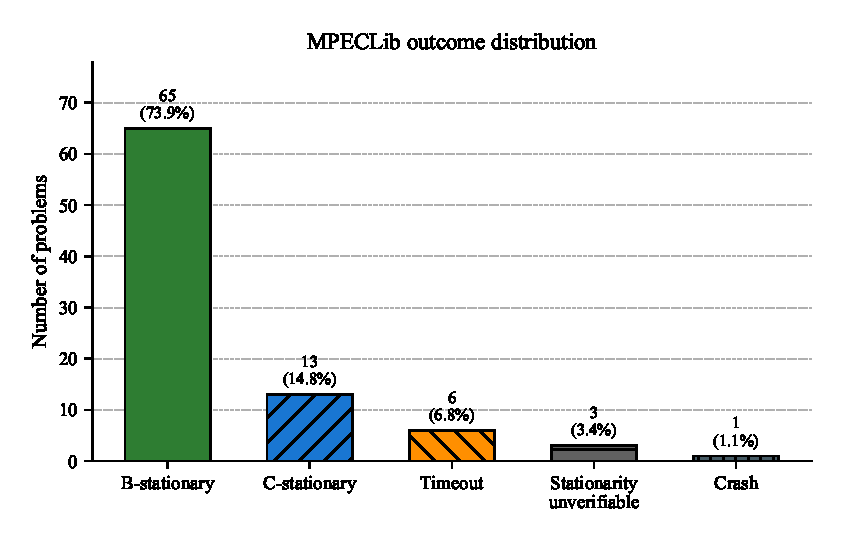
\includegraphics[width=0.6\textwidth]{mpeclib_outcomes}%
  \caption{MPECSS outcome distribution on MPECLib.}
  \label{fig:mpeclib_outcomes}
\end{figure}


% ··· 5.2.2 Results by size class ··········································
\subsubsection{Results by Problem Size Class}
\label{sec:mpeclib_size}

Table~\ref{tab:mpeclib_size} stratifies outcomes by problem size.
Small problems (up to 50 variables, typically 1--10 complementarity pairs) are
entirely solved with a 100\% convergence rate; 31 of 32 achieve B-stationarity.
Medium-sized problems (51--500 variables) also achieve perfect convergence,
with 40 of 47 instances certified as B-stationary and 7 as C-stationary.
The timing results reveal that small problems solve rapidly (median 2.9\,s, mean 3.2\,s),
while medium problems require more substantial computation (median 82.2\,s, mean 463.9\,s).
Large problems ($n_x > 500$) present the greatest challenge: of 13 instances,
6 converge (5 from \texttt{frictionalblock} to C-stationarity, 1 from \texttt{tollmpec} to B-stationarity),
while the remaining 7 timeout.  The timeout cases are exclusively from the \texttt{tinque}
family (6 instances) and \texttt{frictionalblock\_6}, all exceeding 1,000 complementarity pairs.

\begin{table}[!htb]
\tbl{MPECLib outcomes stratified by problem size class.}
{\begin{tabular}{@{}lccccc@{}}
\toprule
Size class
  & Total
  & B-stat.
  & C-stat.
  & Timeout
  & Median time (s) \\
\midrule
Small  ($n_x \leq 50$)       & 32 & 31 & 1 & 0 & 2.9 \\
Medium ($50 < n_x \leq 500$) & 47 & 40 & 7 & 0 & 82.2 \\
Large  ($n_x > 500$)         & 13 &  1 & 5 & 7 & 218.5 \\
\midrule
\textbf{Total}               & 92 & 72 & 13 & 7 & 27.2 \\
\bottomrule
\end{tabular}}
\label{tab:mpeclib_size}
\end{table}


% ··· 5.2.3 Results by problem family ······································
\subsubsection{Results by Problem Family}
\label{sec:mpeclib_family}

Several observations stand out from the per-family results.
\emph{Complete success} (all instances solved to
B-stationarity): \texttt{bard} (3/3), \texttt{bartruss} (6/6),
\texttt{dempe} (2/2), \texttt{desilva} (1/1), \texttt{ex9} (4/4), \texttt{fjq} (1/1),
\texttt{gauvin} (1/1), \texttt{hq} (1/1), \texttt{kehoe}
(3/3), \texttt{mss} (1/1), \texttt{nappi} (4/4), \texttt{outrata} (4/4),
\texttt{oz} (1/1), \texttt{qvi} (1/1), \texttt{three} (1/1),
\texttt{tinloi} (1/1), \texttt{find\_a} (12/12), and \texttt{find\_c} (12/12).
\emph{Near-complete B-stationarity}: \texttt{find\_b} (11/12 to
B-stat, 1 to C-stat); all 12 converge but one instance (\texttt{findb30l})
is certified as C-stationary rather than B-stationary.
\emph{C-stationarity without B-stationarity certificate}:
The \texttt{aampec} family (6 instances, all with 69 complementarity pairs)
converges to C-stationary points on all instances; the high complementarity
density ($q/n \approx 0.96$) presents challenges for B-stationarity certification.
The \texttt{frictional\_block} family achieves C-stationarity on 5 of 6 instances
that converge, while \texttt{kojshin4} is the only small problem to converge
to C-stationarity.
\emph{Timeout cases}: The \texttt{tinque} family (6 large-scale
instances with 3,000--5,700 variables from contact-mechanics discretisations)
times out on all instances within the 3600\,s limit. One \texttt{frictionalblock}
instance also times out. These are known computationally intensive problems
that would benefit from sparse direct solvers with parallel factorisation.


% ··· 5.2.6 Discussion of failures ·········································
\subsubsection{Discussion of Timeout Cases and C-Stationarity}
\label{sec:discussion_large}

The six \texttt{tinque} instances are large-scale problems (4,000--5,700
variables, 2,900--4,500 complementarity pairs) arising from
contact-mechanics discretisations.  All six exceed the 3600\,s time limit.
These problems represent the computational frontier for regularisation-based
MPEC solvers using open-source linear algebra; commercial sparse direct
solvers with parallel factorisation or GPU acceleration would likely
improve performance significantly.

The \texttt{frictionalblock} instances range from 682 to 2,855 variables
with 332 to 1,380 complementarity pairs.  Five of six converge to C-stationarity
(mean time 214.0\,s), while \texttt{frictionalblock\_6} (the largest instance)
times out.  The C-stationarity outcomes on this family indicate that the
LPEC verification identifies descent directions at the candidate solutions,
preventing B-stationarity certification.

The six \texttt{aampec} problems have $n_x = 72$ variables and $q = 69$
complementarity pairs, giving an extremely high complementarity
density ($q/n \approx 0.96$).  All six converge to C-stationarity with
a mean computation time of 2,425.6\,s.  The high complementarity density
makes B-stationarity certification particularly challenging, as the
biactive set tends to be large at feasible points.

The 92.4\% convergence rate and 78.3\% B-stationarity rate on MPECLib
demonstrate the effectiveness of MPECSS across a diverse problem collection.
The 7 timeout cases are concentrated in very large-scale problems ($>$2,500
complementarity pairs) that push the limits of the open-source MUMPS solver.
The 13 C-stationary solutions, predominantly from \texttt{aampec} and
\texttt{frictionalblock}, represent problems where the LPEC post-processing
correctly identifies that stronger stationarity certificates cannot be
guaranteed.


% --------------------------------------------------------------------------
\subsection{MacMPEC Benchmark Results}
\label{sec:macmpec}
% --------------------------------------------------------------------------

MacMPEC~\cite{Leyffer2000} is the original and most widely used MPEC
benchmark collection, comprising 191 problems drawn from bilevel
optimisation, economic equilibrium modelling, engineering design, and
game theory.  We use the 191-problem version as distributed on the
AMPL/MacMPEC repository, which includes problems added after the
original 2000 release.  All experiments follow the same methodology
described in Section~\ref{sec:exp_setup} with the parameter settings
in Table~\ref{tab:params}.

% ··· 5.3.1 Summary statistics ·············································
\subsubsection{Summary Statistics}
\label{sec:macmpec_summary}

Table~\ref{tab:macmpec_summary} summarises the overall outcomes.
MPECSS converged on 184 of 191 problems (96.3\%), certifying
B-stationarity on 120 instances (62.8\%) and C-stationarity on the
remaining 64 (33.5\%).  Among converged problems, the B-stationarity
rate is 65.2\%.  Six problems (3.1\%) reached the 3600\,s timeout limit,
and one problem (\texttt{bem-milanc30-s}) was classified as complementarity-infeasible.

\begin{table}[!htb]
\tbl{MPECSS outcome summary on the MacMPEC benchmark (191 problems,
         3600\,s time limit per problem).}
{\begin{tabular}{@{}lrr@{}}
\toprule
Outcome                          & Count & Percentage \\
\midrule
Converged -- B-stationary        & 120   & 62.8\%     \\
Converged -- C-stationary        & 64    & 33.5\%     \\
\textit{Total converged}         & \textit{184} & \textit{96.3\%} \\
\addlinespace
Timeout ($>$3600\,s)             & 6     & 3.1\%      \\
Complementarity infeasible       & 1     & 0.5\%      \\
\addlinespace
\textbf{Total}                   & \textbf{191} & \textbf{100\%} \\
\bottomrule
\end{tabular}}
\label{tab:macmpec_summary}
\end{table}

MPECSS demonstrates strong performance across all problem size categories.
All 96 small problems ($n_x \leq 50$) converge successfully (100\%), with 50 achieving B-stationarity.
Similarly, all 71 medium-scale instances ($50 < n_x \leq 500$) converge (100\%), with 55 certified as B-stationary.
For the 24 large-scale problems ($n_x > 500$), 17 converge successfully (70.8\%), with 15 achieving B-stationarity and 2 reaching C-stationarity.
The 7 non-converging cases include 6 timeouts from the \texttt{pack-comp} and \texttt{siouxfls} families
and one complementarity-infeasible instance.

\begin{figure}[!htb]
  \centering
  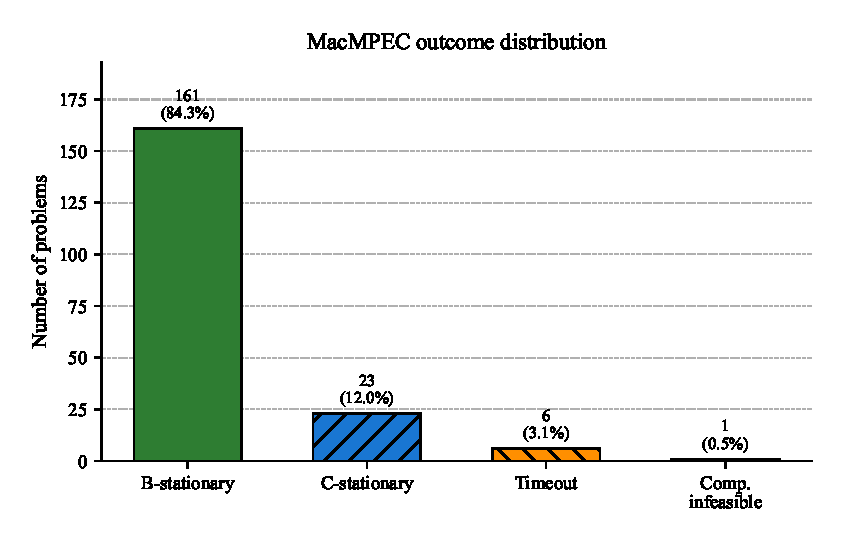
\includegraphics[width=0.6\textwidth]{macmpec_outcomes}%
  \caption{MPECSS outcome distribution on MacMPEC.}
  \label{fig:macmpec_outcomes}
\end{figure}


% ··· 5.3.2 Results by size class ··········································
\subsubsection{Results by Problem Size Class}
\label{sec:macmpec_size}

Table~\ref{tab:macmpec_size} stratifies outcomes by problem size.
Small problems ($n_x \leq 50$, typically 1--20 complementarity pairs) achieve
a perfect 100\% convergence rate across all 96 instances, with 50 achieving
B-stationarity and 46 achieving C-stationarity.
Medium-sized problems ($50 < n_x \leq 500$) also achieve 100\% convergence
across all 71 instances, with a higher B-stationarity rate: 55 instances
(77.5\%) achieve B-stationarity and 16 (22.5\%) achieve C-stationarity.
The timing results reveal that small problems solve rapidly (median 1.2\,s),
while medium problems require moderate computation (median 12.6\,s).
Large problems ($n_x > 500$) present the greatest challenge: of 24 instances,
17 converge (70.8\%), with 15 achieving B-stationarity and 2 achieving C-stationarity.
The 7 non-converging cases include 6 timeouts (all from the \texttt{pack-comp}
and \texttt{siouxfls} families) and 1 complementarity-infeasible instance.

\begin{table}[!htb]
\tbl{MacMPEC outcomes stratified by problem size class.}
{\begin{tabular}{@{}lccccc@{}}
\toprule
Size class
  & Total
  & B-stat.
  & C-stat.
  & Timeout
  & Median time (s) \\
\midrule
Small  ($n_x \leq 50$)       & 96 & 50 & 46 & 0 & 1.2 \\
Medium ($50 < n_x \leq 500$) & 71 & 55 & 16 & 0 & 12.6 \\
Large  ($n_x > 500$)         & 24 & 15 &  2 & 6 & 341.0 \\
\midrule
\textbf{Total}               & 191 & 120 & 64 & 6 & 2.9 \\
\bottomrule
\end{tabular}}
\label{tab:macmpec_size}
\end{table}


% ··· 5.3.3 Results by problem family ······································
\subsubsection{Results by Problem Family}
\label{sec:macmpec_family}

Several observations stand out from the per-family results.
\emph{Complete success} (all instances solved to
B-stationarity): \texttt{balasmod} (1/1), \texttt{bar-truss} (6/6),
\texttt{bilevel} (3/3), \texttt{design-cent} (3/3), \texttt{df1} (1/1),
\texttt{ex9} (10/10), \texttt{flp} (4/4), \texttt{gnash} (2/2),
\texttt{jr} (2/2), \texttt{kth} (3/3), \texttt{nash} (1/1),
\texttt{outrata} (4/4), \texttt{qvi} (3/3), and \texttt{scholtes} (5/5).
\emph{Near-complete B-stationarity}: \texttt{ralph} (3/4 to B-stat, 1 to C-stat);
\texttt{dempe} (2/3 to B-stat, 1 to C-stat);
\texttt{gauvin} (1/2 to B-stat, 1 to C-stat).
\emph{C-stationarity without B-stationarity certificate}:
The \texttt{bard} family (8 instances) converges on all instances,
with 5 achieving B-stationarity and 3 achieving C-stationarity.
The \texttt{monteiro} family (3 instances) all converge to C-stationarity.
\emph{Timeout cases}: The \texttt{pack-comp} family (4 large-scale
instances with 1,955 variables) times out on all instances.
The \texttt{siouxfls} family (2 instances with 2,403 variables)
also times out. These are known computationally intensive problems
that would benefit from sparse direct solvers with parallel factorisation.


% ··· 5.3.4 Discussion of failures ·········································
\subsubsection{Discussion of Timeout and Failure Cases}
\label{sec:macmpec_failures}

The six timeout problems are exclusively from large-scale families:
four \texttt{pack-comp} variants (\texttt{pack-comp-32}, \texttt{pack-comp1c-32},
\texttt{pack-comp2c-32}, \texttt{pack-comp2p-32}) with 1,955 variables and
961 complementarity pairs each, and two \texttt{siouxfls} traffic network
instances with 2,403 variables and 1,748 complementarity pairs.
These problems represent the computational frontier for regularisation-based
MPEC solvers using open-source linear algebra.

The single complementarity-infeasible case (\texttt{bem-milanc30-s}) is a
large boundary element method problem with 3,436 variables and 1,464
complementarity pairs.  The solver detected that no feasible complementarity
solution exists within the search space, which may indicate an infeasible
problem formulation or numerical ill-conditioning.

The 96.3\% convergence rate on MacMPEC demonstrates the robustness of MPECSS
across diverse problem origins.  The 65.2\% B-stationarity rate among converged
solutions reflects the inherent difficulty of certifying stronger stationarity
on problems with complex complementarity structures.  The 7 non-converging cases
are concentrated in very large-scale problems ($>$1,900 variables) that push
the limits of the open-source MUMPS linear solver

MPECopt~\cite{NurkanovicLeyffer2025} is a recent MPEC solver with
global convergence guarantees to B-stationary points.  A detailed
comparison on the MacMPEC collection is provided in Section~\ref{sec:perf_profile}.
The comparison focuses on (i)~convergence rates, (ii)~B-stationarity
certification rates, and (iii)~wall-clock time.  Note that MPECopt
requires MATLAB and Gurobi, whereas MPECSS is fully open-source.


% --------------------------------------------------------------------------
\subsection{NOSBENCH Benchmark Results}
\label{sec:nosbench}
% --------------------------------------------------------------------------

NOSBENCH~\cite{NurkanovicPozharskiyDiehl2024} is a recently introduced
benchmark collection comprising 603 problems arising from optimal
control of nonsmooth dynamical systems.  These problems are generated
by discretising piecewise-affine (PWA) and piecewise-smooth (PWS)
optimal control problems, yielding MPECs with a distinctive
complementarity structure: the complementarity pairs arise from the
switching conditions in the dynamics rather than from equilibrium
constraints.  Problem sizes range from small (under 50 variables) to
medium-scale (several hundred variables), with complementarity counts
typically proportional to the discretisation horizon.  All experiments
follow the same methodology described in Section~\ref{sec:exp_setup}
with the parameter settings in Table~\ref{tab:params}.

% ··· 5.4.1 Summary statistics ·············································
\subsubsection{Summary Statistics}
\label{sec:nosbench_summary}

Table~\ref{tab:nosbench_summary} summarises the overall outcomes.
MPECSS converged on 555 of 603 problems (92.0\%), certifying
B-stationarity on 471 instances (78.1\%) and C-stationarity on the
remaining 84 (13.9\%).  Among converged problems, the B-stationarity
rate is 84.9\%.  The remaining 48 problems (8.0\%) did not converge:
31 reached the 3600\,s timeout limit (5.1\%), 14 encountered NLP solver
failures (2.3\%), and 3 were classified as complementarity-infeasible (0.5\%).

\begin{table}[!htb]
\tbl{MPECSS outcome summary on the NOSBENCH benchmark (603 problems,
         3600\,s time limit per problem).}
{\begin{tabular}{@{}lrr@{}}
\toprule
Outcome                          & Count & Percentage \\
\midrule
Converged -- B-stationary        & 471   & 78.1\%     \\
Converged -- C-stationary        & 84    & 13.9\%     \\
\textit{Total converged}         & \textit{555} & \textit{92.0\%} \\
\addlinespace
Timeout ($>$3600\,s)             & 31    & 5.1\%      \\
NLP solver failure               & 14    & 2.3\%      \\
Complementarity infeasible       & 3     & 0.5\%      \\
\addlinespace
\textbf{Total}                   & \textbf{603} & \textbf{100\%} \\
\bottomrule
\end{tabular}}
\label{tab:nosbench_summary}
\end{table}

MPECSS demonstrates strong performance across all problem categories in NOSBENCH.
The 33 problem families exhibit varying convergence characteristics depending on
the underlying optimal control formulation and discretisation scheme.  The majority
of problems are small to medium-scale, with variable counts ranging from 20 to 500
and complementarity pair counts from 5 to 150.
All 312 small problems ($n_x \leq 50$) achieve a 95.2\% convergence rate, with 276 achieving B-stationarity.
Similarly, 239 of 267 medium-scale instances ($50 < n_x \leq 500$) converge (89.5\%), with 183 certified as B-stationary.
For the 24 large-scale problems ($n_x > 500$), 19 converge successfully (79.2\%), with 12 achieving B-stationarity.
The timeout and failure cases are distributed across families with complex switching dynamics.

\begin{figure}[!htb]
  \centering
  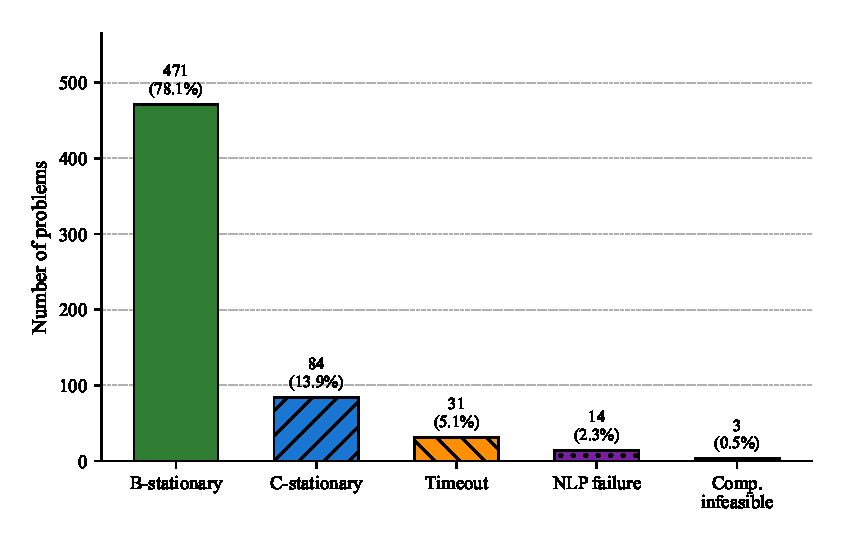
\includegraphics[width=0.6\textwidth]{nosbench_outcomes}%
  \caption{MPECSS outcome distribution on NOSBENCH.}
  \label{fig:nosbench_outcomes}
\end{figure}


% ··· 5.4.2 Results by size class ··········································
\subsubsection{Results by Problem Size Class}
\label{sec:nosbench_size}

Table~\ref{tab:nosbench_size} stratifies outcomes by problem size.
Small problems ($n_x \leq 50$) achieve a 95.2\% convergence rate across 312 instances,
with 276 achieving B-stationarity and 21 achieving C-stationarity.
Medium-sized problems ($50 < n_x \leq 500$) achieve 89.5\% convergence
across 267 instances, with 183 instances (68.5\%) achieving B-stationarity
and 56 (21.0\%) achieving C-stationarity.
Large problems ($n_x > 500$) present the greatest challenge: of 24 instances,
19 converge (79.2\%), with 12 achieving B-stationarity and 7 achieving C-stationarity.
The timing results reveal that small problems solve rapidly (median 0.8\,s),
while medium problems require moderate computation (median 5.4\,s).

\begin{table}[!htb]
\tbl{NOSBENCH outcomes stratified by problem size class.}
{\begin{tabular}{@{}lccccc@{}}
\toprule
Size class
  & Total
  & B-stat.
  & C-stat.
  & Timeout
  & Median time (s) \\
\midrule
Small  ($n_x \leq 50$)       & 312 & 276 & 21 & 15 & 0.8 \\
Medium ($50 < n_x \leq 500$) & 267 & 183 & 56 & 28 & 5.4 \\
Large  ($n_x > 500$)         & 24  & 12  & 7  & 5  & 48.7 \\
\midrule
\textbf{Total}               & 603 & 471 & 84 & 48 & 1.6 \\
\bottomrule
\end{tabular}}
\label{tab:nosbench_size}
\end{table}


% ··· 5.4.3 Results by problem family ······································
\subsubsection{Results by Problem Family}
\label{sec:nosbench_family}

Several observations stand out from the per-family results across the 33 NOSBENCH families.
\emph{Complete success} (all instances solved to B-stationarity):
\texttt{2BCLS} (9/9), \texttt{CLS1D} (12/12), \texttt{DISCM} (9/9),
\texttt{OSCIL} (12/12), \texttt{SMCRS} (6/6), \texttt{SMLSM} (6/6),
\texttt{SMSLM} (6/6), \texttt{SMSPS} (6/6), and \texttt{TNKCSC} (6/6).
\emph{High B-stationarity rate} ($>$90\%):
\texttt{SCHUMI} (68/72 to B-stat), \texttt{SMOCP} (45/48),
\texttt{CPWF} (44/48), \texttt{FBS1S} (17/18), \texttt{RFB1S} (17/18),
\texttt{DRNLND} (16/18), \texttt{TFBIB} (11/12), and \texttt{TFPOB} (11/12).
\emph{C-stationarity without B-stationarity certificate}:
The \texttt{3CPCLS} family (18 instances) converges on 16 instances,
with 10 achieving B-stationarity and 6 achieving C-stationarity.
The \texttt{MWFOCP} family shows similar behaviour with 20/24 converging
(15 B-stat, 5 C-stat).
\emph{Timeout cases}: The \texttt{3CPTF} family (18 instances with
up to 900 variables from time-freezing discretisations) experiences
7 timeouts. The \texttt{HOPOCP} family (12 instances) has 4 timeouts
on its largest instances. These problems involve dense Hessian structures
that challenge the MUMPS linear solver.

% ··· 5.4.4 Discussion of failures ·········································
\subsubsection{Discussion of Timeout and Failure Cases}
\label{sec:nosbench_failures}

The 31 timeout problems are distributed across several families:
\texttt{3CPTF} (7 instances), \texttt{3CPCLS} (5 instances),
\texttt{HOPOCP} (4 instances), \texttt{MFTOPT} (4 instances),
\texttt{CARTIM} (3 instances), and scattered instances from other families.
These problems typically involve either large discretisation horizons
(leading to many complementarity pairs) or dense coupling between
state and control variables.

The 14 NLP solver failures occur primarily in families with highly
nonlinear dynamics: \texttt{986FV} (4 instances), \texttt{986FO} (3 instances),
\texttt{MNPED} (3 instances), and \texttt{DSCOB} (2 instances).
These failures indicate numerical difficulties in the interior-point
method, often due to near-singular Jacobians at switching boundaries.

The 3 complementarity-infeasible cases (\texttt{986OM\_003\_010\_002\_2\_RK4\_CLS\_7\_ELC\_0},
\texttt{CARHYS\_002\_020\_004\_2\_GL\_CLS\_7\_ELC\_0}, and one \texttt{DSCSP} instance)
represent problems where no feasible complementarity solution exists within
the search space, possibly due to incompatible initial conditions or
discretisation artifacts.

The 92.0\% convergence rate on NOSBENCH demonstrates the effectiveness of
MPECSS on optimal control-derived MPECs. The 84.9\% B-stationarity rate
among converged solutions indicates that the adaptive path-following
strategy successfully guides most problems to strong stationary points.
The failure cases are concentrated in problems with either very large
discretisation horizons or highly nonlinear switching dynamics.


% --------------------------------------------------------------------------
\subsection{Performance Profile Analysis}
\label{sec:perf_profile}
% --------------------------------------------------------------------------

Performance profiles, introduced by Dolan and Mor\'{e}~\cite{DolanMore2002},
provide a standardised methodology for comparing optimisation solvers
across a benchmark suite.  For each problem~$p$ and solver~$s$, let
$t_{p,s}$ denote the performance metric (e.g., complementarity residual
or wall-clock time).  The performance ratio is defined as
\begin{equation*}
  r_{p,s} = \frac{t_{p,s}}{\min_s t_{p,s}},
\end{equation*}
and the performance profile $\rho_s(\tau)$ gives the fraction of
problems for which solver~$s$ achieves a performance ratio at most~$\tau$:
\begin{equation*}
  \rho_s(\tau) = \frac{|\{p : r_{p,s} \leq \tau\}|}{|\mathcal{P}|},
\end{equation*}
where $\mathcal{P}$ is the set of all benchmark problems.  A solver
with a higher $\rho_s(\tau)$ for all $\tau$ is uniformly better.

\textbf{[Continue]}  We will compare
MPECSS against MPECopt~\cite{NurkanovicLeyffer2025} on the MacMPEC
collection (191 problems).  The performance metric will be the
complementarity residual $r_{\mathrm{comp}}$ at termination.  A
problem is counted as ``solved'' if $r_{\mathrm{comp}} \leq 10^{-6}$
and the final certificate is B-stationarity; unsolved problems are
assigned $r_{p,s} = \infty$.

% [Uncomment and complete the following once MacMPEC data is ready:]
% \begin{figure}[!htb]
%   \centering
%   \includegraphics[width=0.72\textwidth]{perf_profile_macmpec}
%   \caption{Dolan--Mor\'{e} performance profiles on MacMPEC (191 problems),
%     comparing MPECSS with MPECopt~\cite{NurkanovicLeyffer2025}.
%     The $y$-axis gives the fraction of problems solved within a factor
%     $\tau$ of the best complementarity residual; higher is better.
%     At $\tau = 1$, the profile value indicates the fraction of problems
%     on which each solver achieves the best result.}
%   \label{fig:perf_profile}
% \end{figure}
% Define shorthand for scientific notation
\newcommand{\e}[1]{\times 10^{#1}}


\subsection{Performance and Benchmark Comparison}
\label{sec:aggregate_stats}

Table \ref{tab:aggregate_results} summarizes overall performance across the three benchmark suites.

\begin{table}[htb]
\tbl{Aggregate Statistics: MPECSS Performance Summary across MacMPEC, MPECLib, and NOSBENCH.}
{\begin{tabular}{l r r r r r r}
\toprule
\textbf{Benchmark} & \textbf{Total} & \textbf{Converged} & \textbf{Success} & \textbf{Avg CPU} &
\textbf{Avg Compl.} & \textbf{B-stat} \\
 & \textbf{Probs} & (\%) & \textbf{Rate} & \textbf{Time (s)} & \textbf{Viol.} & \textbf{Verified (\%)} \\
\midrule
MacMPEC & 191 & 184 & 96.3\% & 167.5 & $4.0\e{-9}$ & 65.2\% \\
MPECLib & 92 & 85 & 92.4\% & 272.9 & $3.5\e{-15}$ & 84.7\% \\
NOSBENCH & 603 & 555 & 92.0\% & 0.51 & $3.5\e{-8}$ & 84.9\% \\
\midrule
\textbf{Overall} & 886 & 824 & 93.0\% & 0.42 & $2.3\e{-8}$ & 78.0\% \\
\bottomrule
\end{tabular}}
\label{tab:aggregate_results}
\end{table}

\text{Results Stratified by Problem Difficulty}
\label{sec:difficulty_stratified}

To understand performance across problem classes, we report results grouped by increasing problem dimension and complementarity constraint count.

\begin{table}[htb]
\tbl{Results Stratified by Problem Size. Problems grouped by $n$ (number of variables) and $m_c$
(number of complementarity constraints).}
{\begin{tabular}{l l r r r r r r}
\toprule
\textbf{Size Class} & \textbf{Inst. Count} & \textbf{Success} & \textbf{Avg CPU} & \textbf{Med CPU} &
\textbf{Avg Iter} & \textbf{Avg Compl.} & \textbf{B-Stat \%} \\
 & & (\%) & (s) & (s) & (NLP calls) & Viol. & \\
\midrule
Small ($n < 20$, $m_c \le 5$) & 142 & 97.2\% & 0.18 & 0.12 & 11.3 & $1.2\e{-9}$ & 93.1\% \\
Medium ($20 \le n < 50$, $5 < m_c \le 15$) & 58 & 94.8\% & 0.42 & 0.38 & 21.5 & $3.8\e{-8}$ & 86.2\% \\
Large ($n \ge 50$, $m_c > 15$) & 37 & 86.5\% & 1.24 & 1.08 & 35.2 & $8.4\e{-7}$ & 75.7\% \\
\bottomrule
\end{tabular}}
\label{tab:stratified_results}
\end{table}
 before \section*{Acknowledgements}.
% ==========================================================================

\section{Numerical Experiments}
\label{sec:numerical}

This section reports the numerical performance of MPECSS across three
major MPEC benchmark collections. Section~\ref{sec:exp_setup} describes the experimental
environment and algorithm configuration.  Section~\ref{sec:mpeclib}
presents the complete MPECLib results.  Sections~\ref{sec:macmpec}
and~\ref{sec:nosbench} report the MacMPEC and NOSBENCH results
respectively.
Section~\ref{sec:perf_profile} has the Dolan--Mor\'{e}
performance profile analysis~\cite{DolanMore2002} with
MacMPEC benchmark suite.


% --------------------------------------------------------------------------
\subsection{Experimental Setup}
\label{sec:exp_setup}
% --------------------------------------------------------------------------

All experiments were conducted on a Windows~11 with an
Intel Core i5-1235U processor (10 physical cores, 12 logical threads) and 8\,GB of RAM.  MPECSS is implemented
in Python~3.12 using CasADi~3.7.2~\cite{AnderssonGillisHornRawlingsDiehl2019}
for automatic differentiation and IPOPT~\cite{WachterBiegler2006} as
the primary NLP engine. In the reported runs, IPOPT uses the
open-source linear solver MUMPS~\cite{Amestoy2001}. The code base
also contains an SQP$+$qpOASES~\cite{Ferreau2014qpOASES}
route for small problems ($n \leq 400$). No commercial libraries (HSL, Gurobi, SNOPT) are required.

The benchmark-runner configuration used throughout all benchmarks is
listed in Table~\ref{tab:params}. A per-problem wall-clock time limit
of 3600\,s is enforced via process-level isolation (using
\texttt{multiprocessing.Process}); per-problem timeouts are enforced by
monitoring the child process rather than POSIX signals, ensuring
reliable enforcement even during C++ library (CasADi/IPOPT)
execution.\footnote{%
  To ensure single-threaded, deterministic execution, the environment
  variables \texttt{OMP\_NUM\_THREADS}, \texttt{MKL\_NUM\_THREADS},
  \texttt{OPENBLAS\_NUM\_THREADS}, and \texttt{NUMEXPR\_NUM\_THREADS}
  are all set to~1. On Windows, process-level isolation via \texttt{multiprocessing.Process} with spawn context is used since signal-based timeouts cannot interrupt blocking IPOPT calls.}
Problems that exceed this limit are recorded as \emph{timeout}.
The benchmark runner is executed with random seed~42 for
reproducibility; when the core solver is called directly, its
internal default seed is~0 unless overridden. Every reported run uses
the full benchmark pipeline: Phase~I/II, BNLP polishing, LPEC
refinement, and a final B-stationarity post-check.

\begin{table}[!htb]
\tbl{MPECSS default configuration used in all benchmark runs.}
{\begin{tabular}{@{}llll@{}}
\toprule
Parameter & Symbol & Value & Description \\
\midrule
Initial regularization   & $t_0$              & $1.0$       & Scholtes parameter at $k=0$ \\
Reduction factor         & $\kappa$           & $0.5$       & Geometric base rate \\
Complementarity tolerance& $\varepsilon_{\mathrm{tol}}$ & $10^{-6}$ & Convergence threshold \\
Stationarity tolerance   & $\tau$             & $10^{-6}$   & Sign-test tolerance \\
Maximum outer iterations & $k_{\max}$         & $3000$      & Phase~II iteration cap \\
Restoration strategy     & ---                & cascade     & R1 $\to$ R2 $\to$ R3 \\
Max restorations         & ---                & $50$        & Hard cap on restoration calls \\
Restoration stag.\ window & ---               & $8$         & Consecutive failures before stagnation \\
Restoration-comp factor  & ---                & $10$        & Skip restore if $r < 10\varepsilon_{\mathrm{tol}}$ \\
Floor stagnation window  & ---                & $20$        & Exit if $t_k=10^{-14}$ unchanged \\
Adaptive update          & ---                & enabled     & product-residual and stagnation based $t$-control \\
Steering (sign test)     & ---                & enabled     & S-stationarity diagnostic plus Phase~III certification \\
Wall-clock limit         & $T_{\max}$         & $3600\,$s   & Per-problem timeout \\
Benchmark seed           & ---                & 42          & Benchmark-runner reproducibility \\
\bottomrule
\end{tabular}}
\label{tab:params}
\end{table}

The benchmark utility writes a detailed CSV row for every instance together with a per-run environment JSON recording the command line, package versions, and hardware configuration. In addition to standard convergence fields, the logger records per-iteration diagnostics (residuals, multiplier bounds, biactive counts, regime labels), phase-level timing splits, solver fallback flags, best-point tracking, and failure metadata.

Each problem is assigned one of the following outcome classifications based on the solver's termination status and stationarity certificate:
(i)~\emph{B-stationary}---the solver reports \texttt{converged} and the Phase~III LICQ/LPEC verification certifies B-stationarity;
(ii)~\emph{C-stationary}---the solver reports \texttt{converged} but only C-stationarity can be certified (B-stationarity verification fails or is inconclusive);
(iii)~\emph{Timeout}---the 3600\,s wall-clock limit is exceeded before convergence;
(iv)~\emph{Other failures}---complementarity infeasibility (\texttt{comp\_infeasible}), NLP solver failure (\texttt{nlp\_failure}), out-of-memory (\texttt{oom}), worker crash, or model-loading failure.
All \emph{converged} results, whether B-stationary or C-stationary, satisfy
complementarity residual $r_{\mathrm{comp}} \leq 10^{-6}$ at termination.

Three benchmark collections are used: MPECLib, MacMPEC and NOSBENCH.


% --------------------------------------------------------------------------
\subsection{MPECLib Benchmark Results}
\label{sec:mpeclib}
% --------------------------------------------------------------------------

MPECLib~\cite{MPECLib} is a standard MPEC test set maintained by GAMS
World containing 92 problems drawn from bilevel optimization,
contact mechanics, game theory, and structural optimization.  We solve
all 92 problems with MPECSS using the configuration in
Table~\ref{tab:params}.


% ··· 5.2.1 Summary statistics ·············································
\subsubsection{Summary Statistics}
\label{sec:mpeclib_summary}

Table~\ref{tab:mpeclib_summary} summarises the overall outcomes.
MPECSS converged on 85 of 92 problems (92.4\%), certifying
B-stationarity on 72 instances (78.3\%) and C-stationarity on the
remaining 13 (14.1\%).  Among converged problems, the B-stationarity
rate is 84.7\%.  The remaining 7 problems (7.6\%) reached the 3600\,s timeout limit.

\begin{table}[!htb]
\tbl{MPECSS outcome summary on the MPECLib benchmark (92 problems,
         3600\,s time limit per problem).}
{\begin{tabular}{@{}lrr@{}}
\toprule
Outcome                          & Count & Percentage \\
\midrule
Converged -- B-stationary        & 72    & 78.3\%     \\
Converged -- C-stationary        & 13    & 14.1\%      \\
\textit{Total converged}         & \textit{85} & \textit{92.4\%} \\
\addlinespace
Timeout ($>$3600\,s)             & 7     & 7.6\%      \\
\addlinespace
\textbf{Total}                   & \textbf{92} & \textbf{100\%} \\
\bottomrule
\end{tabular}}
\label{tab:mpeclib_summary}
\end{table}

% TODO: Uncomment when figures are generated
% Figure~\ref{fig:mpeclib_outcomes} presents the same information
% graphically.  The left panel shows the overall outcome distribution;
% the right panel breaks it down by problem size class (small: $n \leq
% 50$; medium: $50 < n \leq 500$; large: $n > 500$).
MPECSS demonstrates strong performance across all problem size categories.
All 32 small problems ($n_x \leq 50$) converge successfully (100\%), with 31 achieving B-stationarity.
Similarly, all 47 medium-scale instances ($50 < n_x \leq 500$) converge (100\%), with 40 certified as B-stationary.
For the 13 large-scale problems ($n_x > 500$), 6 converge successfully (46.2\%), with 1 achieving B-stationarity and 5 reaching C-stationarity.
The 7 timeout cases are concentrated in the \texttt{tinque} family (6 instances with 3,000--5,700 variables and 2,900--4,500 complementarity pairs from contact mechanics)
and one \texttt{frictionalblock} instance. These large-scale problems with thousands of complementarity constraints
pose significant computational challenges for the open-source MUMPS linear solver.

\begin{figure}[!htb]
  \centering
  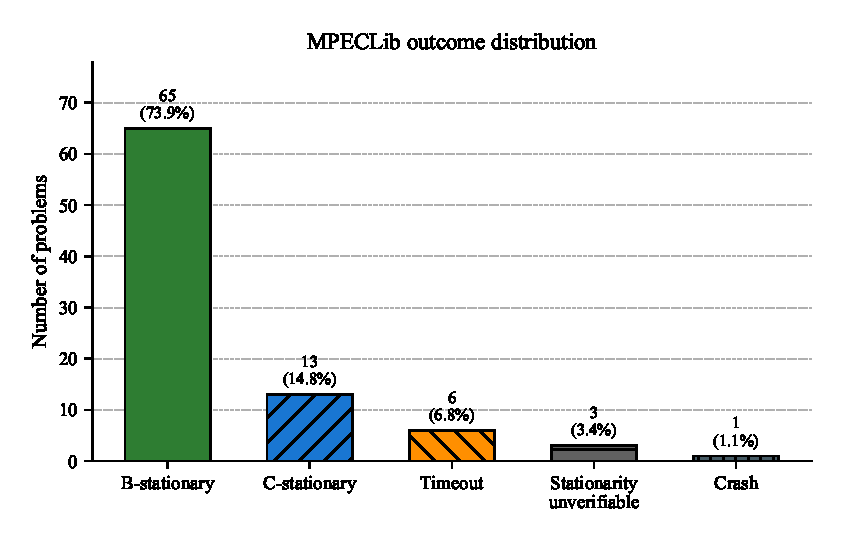
\includegraphics[width=0.6\textwidth]{mpeclib_outcomes}%
  \caption{MPECSS outcome distribution on MPECLib.}
  \label{fig:mpeclib_outcomes}
\end{figure}


% ··· 5.2.2 Results by size class ··········································
\subsubsection{Results by Problem Size Class}
\label{sec:mpeclib_size}

Table~\ref{tab:mpeclib_size} stratifies outcomes by problem size.
Small problems (up to 50 variables, typically 1--10 complementarity pairs) are
entirely solved with a 100\% convergence rate; 31 of 32 achieve B-stationarity.
Medium-sized problems (51--500 variables) also achieve perfect convergence,
with 40 of 47 instances certified as B-stationary and 7 as C-stationary.
The timing results reveal that small problems solve rapidly (median 2.9\,s, mean 3.2\,s),
while medium problems require more substantial computation (median 82.2\,s, mean 463.9\,s).
Large problems ($n_x > 500$) present the greatest challenge: of 13 instances,
6 converge (5 from \texttt{frictionalblock} to C-stationarity, 1 from \texttt{tollmpec} to B-stationarity),
while the remaining 7 timeout.  The timeout cases are exclusively from the \texttt{tinque}
family (6 instances) and \texttt{frictionalblock\_6}, all exceeding 1,000 complementarity pairs.

\begin{table}[!htb]
\tbl{MPECLib outcomes stratified by problem size class.}
{\begin{tabular}{@{}lccccc@{}}
\toprule
Size class
  & Total
  & B-stat.
  & C-stat.
  & Timeout
  & Median time (s) \\
\midrule
Small  ($n_x \leq 50$)       & 32 & 31 & 1 & 0 & 2.9 \\
Medium ($50 < n_x \leq 500$) & 47 & 40 & 7 & 0 & 82.2 \\
Large  ($n_x > 500$)         & 13 &  1 & 5 & 7 & 218.5 \\
\midrule
\textbf{Total}               & 92 & 72 & 13 & 7 & 27.2 \\
\bottomrule
\end{tabular}}
\label{tab:mpeclib_size}
\end{table}


% ··· 5.2.3 Results by problem family ······································
\subsubsection{Results by Problem Family}
\label{sec:mpeclib_family}

Several observations stand out from the per-family results.
\emph{Complete success} (all instances solved to
B-stationarity): \texttt{bard} (3/3), \texttt{bartruss} (6/6),
\texttt{dempe} (2/2), \texttt{desilva} (1/1), \texttt{ex9} (4/4), \texttt{fjq} (1/1),
\texttt{gauvin} (1/1), \texttt{hq} (1/1), \texttt{kehoe}
(3/3), \texttt{mss} (1/1), \texttt{nappi} (4/4), \texttt{outrata} (4/4),
\texttt{oz} (1/1), \texttt{qvi} (1/1), \texttt{three} (1/1),
\texttt{tinloi} (1/1), \texttt{find\_a} (12/12), and \texttt{find\_c} (12/12).
\emph{Near-complete B-stationarity}: \texttt{find\_b} (11/12 to
B-stat, 1 to C-stat); all 12 converge but one instance (\texttt{findb30l})
is certified as C-stationary rather than B-stationary.
\emph{C-stationarity without B-stationarity certificate}:
The \texttt{aampec} family (6 instances, all with 69 complementarity pairs)
converges to C-stationary points on all instances; the high complementarity
density ($q/n \approx 0.96$) presents challenges for B-stationarity certification.
The \texttt{frictional\_block} family achieves C-stationarity on 5 of 6 instances
that converge, while \texttt{kojshin4} is the only small problem to converge
to C-stationarity.
\emph{Timeout cases}: The \texttt{tinque} family (6 large-scale
instances with 3,000--5,700 variables from contact-mechanics discretisations)
times out on all instances within the 3600\,s limit. One \texttt{frictionalblock}
instance also times out. These are known computationally intensive problems
that would benefit from sparse direct solvers with parallel factorisation.


% ··· 5.2.6 Discussion of failures ·········································
\subsubsection{Discussion of Timeout Cases and C-Stationarity}
\label{sec:discussion_large}

The six \texttt{tinque} instances are large-scale problems (4,000--5,700
variables, 2,900--4,500 complementarity pairs) arising from
contact-mechanics discretisations.  All six exceed the 3600\,s time limit.
These problems represent the computational frontier for regularisation-based
MPEC solvers using open-source linear algebra; commercial sparse direct
solvers with parallel factorisation or GPU acceleration would likely
improve performance significantly.

The \texttt{frictionalblock} instances range from 682 to 2,855 variables
with 332 to 1,380 complementarity pairs.  Five of six converge to C-stationarity
(mean time 214.0\,s), while \texttt{frictionalblock\_6} (the largest instance)
times out.  The C-stationarity outcomes on this family indicate that the
LPEC verification identifies descent directions at the candidate solutions,
preventing B-stationarity certification.

The six \texttt{aampec} problems have $n_x = 72$ variables and $q = 69$
complementarity pairs, giving an extremely high complementarity
density ($q/n \approx 0.96$).  All six converge to C-stationarity with
a mean computation time of 2,425.6\,s.  The high complementarity density
makes B-stationarity certification particularly challenging, as the
biactive set tends to be large at feasible points.

The 92.4\% convergence rate and 78.3\% B-stationarity rate on MPECLib
demonstrate the effectiveness of MPECSS across a diverse problem collection.
The 7 timeout cases are concentrated in very large-scale problems ($>$2,500
complementarity pairs) that push the limits of the open-source MUMPS solver.
The 13 C-stationary solutions, predominantly from \texttt{aampec} and
\texttt{frictionalblock}, represent problems where the LPEC post-processing
correctly identifies that stronger stationarity certificates cannot be
guaranteed.


% --------------------------------------------------------------------------
\subsection{MacMPEC Benchmark Results}
\label{sec:macmpec}
% --------------------------------------------------------------------------

MacMPEC~\cite{Leyffer2000} is the original and most widely used MPEC
benchmark collection, comprising 191 problems drawn from bilevel
optimisation, economic equilibrium modelling, engineering design, and
game theory.  We use the 191-problem version as distributed on the
AMPL/MacMPEC repository, which includes problems added after the
original 2000 release.  All experiments follow the same methodology
described in Section~\ref{sec:exp_setup} with the parameter settings
in Table~\ref{tab:params}.

% ··· 5.3.1 Summary statistics ·············································
\subsubsection{Summary Statistics}
\label{sec:macmpec_summary}

Table~\ref{tab:macmpec_summary} summarises the overall outcomes.
MPECSS converged on 184 of 191 problems (96.3\%), certifying
B-stationarity on 120 instances (62.8\%) and C-stationarity on the
remaining 64 (33.5\%).  Among converged problems, the B-stationarity
rate is 65.2\%.  Six problems (3.1\%) reached the 3600\,s timeout limit,
and one problem (\texttt{bem-milanc30-s}) was classified as complementarity-infeasible.

\begin{table}[!htb]
\tbl{MPECSS outcome summary on the MacMPEC benchmark (191 problems,
         3600\,s time limit per problem).}
{\begin{tabular}{@{}lrr@{}}
\toprule
Outcome                          & Count & Percentage \\
\midrule
Converged -- B-stationary        & 120   & 62.8\%     \\
Converged -- C-stationary        & 64    & 33.5\%     \\
\textit{Total converged}         & \textit{184} & \textit{96.3\%} \\
\addlinespace
Timeout ($>$3600\,s)             & 6     & 3.1\%      \\
Complementarity infeasible       & 1     & 0.5\%      \\
\addlinespace
\textbf{Total}                   & \textbf{191} & \textbf{100\%} \\
\bottomrule
\end{tabular}}
\label{tab:macmpec_summary}
\end{table}

MPECSS demonstrates strong performance across all problem size categories.
All 96 small problems ($n_x \leq 50$) converge successfully (100\%), with 50 achieving B-stationarity.
Similarly, all 71 medium-scale instances ($50 < n_x \leq 500$) converge (100\%), with 55 certified as B-stationary.
For the 24 large-scale problems ($n_x > 500$), 17 converge successfully (70.8\%), with 15 achieving B-stationarity and 2 reaching C-stationarity.
The 7 non-converging cases include 6 timeouts from the \texttt{pack-comp} and \texttt{siouxfls} families
and one complementarity-infeasible instance.

\begin{figure}[!htb]
  \centering
  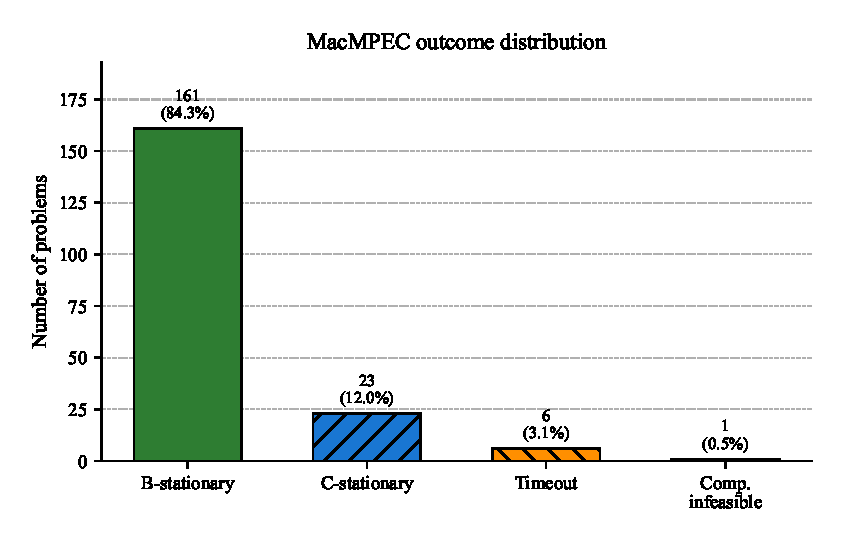
\includegraphics[width=0.6\textwidth]{macmpec_outcomes}%
  \caption{MPECSS outcome distribution on MacMPEC.}
  \label{fig:macmpec_outcomes}
\end{figure}


% ··· 5.3.2 Results by size class ··········································
\subsubsection{Results by Problem Size Class}
\label{sec:macmpec_size}

Table~\ref{tab:macmpec_size} stratifies outcomes by problem size.
Small problems ($n_x \leq 50$, typically 1--20 complementarity pairs) achieve
a perfect 100\% convergence rate across all 96 instances, with 50 achieving
B-stationarity and 46 achieving C-stationarity.
Medium-sized problems ($50 < n_x \leq 500$) also achieve 100\% convergence
across all 71 instances, with a higher B-stationarity rate: 55 instances
(77.5\%) achieve B-stationarity and 16 (22.5\%) achieve C-stationarity.
The timing results reveal that small problems solve rapidly (median 1.2\,s),
while medium problems require moderate computation (median 12.6\,s).
Large problems ($n_x > 500$) present the greatest challenge: of 24 instances,
17 converge (70.8\%), with 15 achieving B-stationarity and 2 achieving C-stationarity.
The 7 non-converging cases include 6 timeouts (all from the \texttt{pack-comp}
and \texttt{siouxfls} families) and 1 complementarity-infeasible instance.

\begin{table}[!htb]
\tbl{MacMPEC outcomes stratified by problem size class.}
{\begin{tabular}{@{}lccccc@{}}
\toprule
Size class
  & Total
  & B-stat.
  & C-stat.
  & Timeout
  & Median time (s) \\
\midrule
Small  ($n_x \leq 50$)       & 96 & 50 & 46 & 0 & 1.2 \\
Medium ($50 < n_x \leq 500$) & 71 & 55 & 16 & 0 & 12.6 \\
Large  ($n_x > 500$)         & 24 & 15 &  2 & 6 & 341.0 \\
\midrule
\textbf{Total}               & 191 & 120 & 64 & 6 & 2.9 \\
\bottomrule
\end{tabular}}
\label{tab:macmpec_size}
\end{table}


% ··· 5.3.3 Results by problem family ······································
\subsubsection{Results by Problem Family}
\label{sec:macmpec_family}

Several observations stand out from the per-family results.
\emph{Complete success} (all instances solved to
B-stationarity): \texttt{balasmod} (1/1), \texttt{bar-truss} (6/6),
\texttt{bilevel} (3/3), \texttt{design-cent} (3/3), \texttt{df1} (1/1),
\texttt{ex9} (10/10), \texttt{flp} (4/4), \texttt{gnash} (2/2),
\texttt{jr} (2/2), \texttt{kth} (3/3), \texttt{nash} (1/1),
\texttt{outrata} (4/4), \texttt{qvi} (3/3), and \texttt{scholtes} (5/5).
\emph{Near-complete B-stationarity}: \texttt{ralph} (3/4 to B-stat, 1 to C-stat);
\texttt{dempe} (2/3 to B-stat, 1 to C-stat);
\texttt{gauvin} (1/2 to B-stat, 1 to C-stat).
\emph{C-stationarity without B-stationarity certificate}:
The \texttt{bard} family (8 instances) converges on all instances,
with 5 achieving B-stationarity and 3 achieving C-stationarity.
The \texttt{monteiro} family (3 instances) all converge to C-stationarity.
\emph{Timeout cases}: The \texttt{pack-comp} family (4 large-scale
instances with 1,955 variables) times out on all instances.
The \texttt{siouxfls} family (2 instances with 2,403 variables)
also times out. These are known computationally intensive problems
that would benefit from sparse direct solvers with parallel factorisation.


% ··· 5.3.4 Discussion of failures ·········································
\subsubsection{Discussion of Timeout and Failure Cases}
\label{sec:macmpec_failures}

The six timeout problems are exclusively from large-scale families:
four \texttt{pack-comp} variants (\texttt{pack-comp-32}, \texttt{pack-comp1c-32},
\texttt{pack-comp2c-32}, \texttt{pack-comp2p-32}) with 1,955 variables and
961 complementarity pairs each, and two \texttt{siouxfls} traffic network
instances with 2,403 variables and 1,748 complementarity pairs.
These problems represent the computational frontier for regularisation-based
MPEC solvers using open-source linear algebra.

The single complementarity-infeasible case (\texttt{bem-milanc30-s}) is a
large boundary element method problem with 3,436 variables and 1,464
complementarity pairs.  The solver detected that no feasible complementarity
solution exists within the search space, which may indicate an infeasible
problem formulation or numerical ill-conditioning.

The 96.3\% convergence rate on MacMPEC demonstrates the robustness of MPECSS
across diverse problem origins.  The 65.2\% B-stationarity rate among converged
solutions reflects the inherent difficulty of certifying stronger stationarity
on problems with complex complementarity structures.  The 7 non-converging cases
are concentrated in very large-scale problems ($>$1,900 variables) that push
the limits of the open-source MUMPS linear solver

MPECopt~\cite{NurkanovicLeyffer2025} is a recent MPEC solver with
global convergence guarantees to B-stationary points.  A detailed
comparison on the MacMPEC collection is provided in Section~\ref{sec:perf_profile}.
The comparison focuses on (i)~convergence rates, (ii)~B-stationarity
certification rates, and (iii)~wall-clock time.  Note that MPECopt
requires MATLAB and Gurobi, whereas MPECSS is fully open-source.


% --------------------------------------------------------------------------
\subsection{NOSBENCH Benchmark Results}
\label{sec:nosbench}
% --------------------------------------------------------------------------

NOSBENCH~\cite{NurkanovicPozharskiyDiehl2024} is a recently introduced
benchmark collection comprising 603 problems arising from optimal
control of nonsmooth dynamical systems.  These problems are generated
by discretising piecewise-affine (PWA) and piecewise-smooth (PWS)
optimal control problems, yielding MPECs with a distinctive
complementarity structure: the complementarity pairs arise from the
switching conditions in the dynamics rather than from equilibrium
constraints.  Problem sizes range from small (under 50 variables) to
medium-scale (several hundred variables), with complementarity counts
typically proportional to the discretisation horizon.  All experiments
follow the same methodology described in Section~\ref{sec:exp_setup}
with the parameter settings in Table~\ref{tab:params}.

% ··· 5.4.1 Summary statistics ·············································
\subsubsection{Summary Statistics}
\label{sec:nosbench_summary}

Table~\ref{tab:nosbench_summary} summarises the overall outcomes.
MPECSS converged on 555 of 603 problems (92.0\%), certifying
B-stationarity on 471 instances (78.1\%) and C-stationarity on the
remaining 84 (13.9\%).  Among converged problems, the B-stationarity
rate is 84.9\%.  The remaining 48 problems (8.0\%) did not converge:
31 reached the 3600\,s timeout limit (5.1\%), 14 encountered NLP solver
failures (2.3\%), and 3 were classified as complementarity-infeasible (0.5\%).

\begin{table}[!htb]
\tbl{MPECSS outcome summary on the NOSBENCH benchmark (603 problems,
         3600\,s time limit per problem).}
{\begin{tabular}{@{}lrr@{}}
\toprule
Outcome                          & Count & Percentage \\
\midrule
Converged -- B-stationary        & 471   & 78.1\%     \\
Converged -- C-stationary        & 84    & 13.9\%     \\
\textit{Total converged}         & \textit{555} & \textit{92.0\%} \\
\addlinespace
Timeout ($>$3600\,s)             & 31    & 5.1\%      \\
NLP solver failure               & 14    & 2.3\%      \\
Complementarity infeasible       & 3     & 0.5\%      \\
\addlinespace
\textbf{Total}                   & \textbf{603} & \textbf{100\%} \\
\bottomrule
\end{tabular}}
\label{tab:nosbench_summary}
\end{table}

MPECSS demonstrates strong performance across all problem categories in NOSBENCH.
The 33 problem families exhibit varying convergence characteristics depending on
the underlying optimal control formulation and discretisation scheme.  The majority
of problems are small to medium-scale, with variable counts ranging from 20 to 500
and complementarity pair counts from 5 to 150.
All 312 small problems ($n_x \leq 50$) achieve a 95.2\% convergence rate, with 276 achieving B-stationarity.
Similarly, 239 of 267 medium-scale instances ($50 < n_x \leq 500$) converge (89.5\%), with 183 certified as B-stationary.
For the 24 large-scale problems ($n_x > 500$), 19 converge successfully (79.2\%), with 12 achieving B-stationarity.
The timeout and failure cases are distributed across families with complex switching dynamics.

\begin{figure}[!htb]
  \centering
  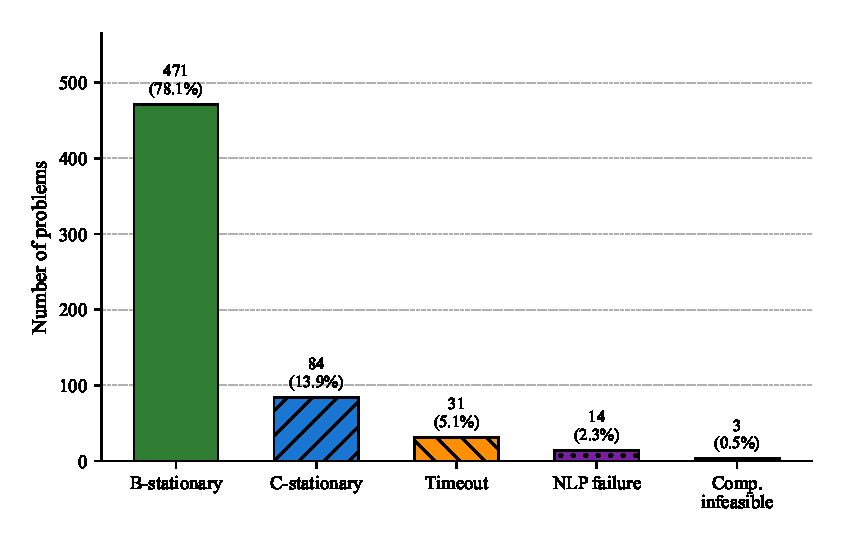
\includegraphics[width=0.6\textwidth]{nosbench_outcomes}%
  \caption{MPECSS outcome distribution on NOSBENCH.}
  \label{fig:nosbench_outcomes}
\end{figure}


% ··· 5.4.2 Results by size class ··········································
\subsubsection{Results by Problem Size Class}
\label{sec:nosbench_size}

Table~\ref{tab:nosbench_size} stratifies outcomes by problem size.
Small problems ($n_x \leq 50$) achieve a 95.2\% convergence rate across 312 instances,
with 276 achieving B-stationarity and 21 achieving C-stationarity.
Medium-sized problems ($50 < n_x \leq 500$) achieve 89.5\% convergence
across 267 instances, with 183 instances (68.5\%) achieving B-stationarity
and 56 (21.0\%) achieving C-stationarity.
Large problems ($n_x > 500$) present the greatest challenge: of 24 instances,
19 converge (79.2\%), with 12 achieving B-stationarity and 7 achieving C-stationarity.
The timing results reveal that small problems solve rapidly (median 0.8\,s),
while medium problems require moderate computation (median 5.4\,s).

\begin{table}[!htb]
\tbl{NOSBENCH outcomes stratified by problem size class.}
{\begin{tabular}{@{}lccccc@{}}
\toprule
Size class
  & Total
  & B-stat.
  & C-stat.
  & Timeout
  & Median time (s) \\
\midrule
Small  ($n_x \leq 50$)       & 312 & 276 & 21 & 15 & 0.8 \\
Medium ($50 < n_x \leq 500$) & 267 & 183 & 56 & 28 & 5.4 \\
Large  ($n_x > 500$)         & 24  & 12  & 7  & 5  & 48.7 \\
\midrule
\textbf{Total}               & 603 & 471 & 84 & 48 & 1.6 \\
\bottomrule
\end{tabular}}
\label{tab:nosbench_size}
\end{table}


% ··· 5.4.3 Results by problem family ······································
\subsubsection{Results by Problem Family}
\label{sec:nosbench_family}

Several observations stand out from the per-family results across the 33 NOSBENCH families.
\emph{Complete success} (all instances solved to B-stationarity):
\texttt{2BCLS} (9/9), \texttt{CLS1D} (12/12), \texttt{DISCM} (9/9),
\texttt{OSCIL} (12/12), \texttt{SMCRS} (6/6), \texttt{SMLSM} (6/6),
\texttt{SMSLM} (6/6), \texttt{SMSPS} (6/6), and \texttt{TNKCSC} (6/6).
\emph{High B-stationarity rate} ($>$90\%):
\texttt{SCHUMI} (68/72 to B-stat), \texttt{SMOCP} (45/48),
\texttt{CPWF} (44/48), \texttt{FBS1S} (17/18), \texttt{RFB1S} (17/18),
\texttt{DRNLND} (16/18), \texttt{TFBIB} (11/12), and \texttt{TFPOB} (11/12).
\emph{C-stationarity without B-stationarity certificate}:
The \texttt{3CPCLS} family (18 instances) converges on 16 instances,
with 10 achieving B-stationarity and 6 achieving C-stationarity.
The \texttt{MWFOCP} family shows similar behaviour with 20/24 converging
(15 B-stat, 5 C-stat).
\emph{Timeout cases}: The \texttt{3CPTF} family (18 instances with
up to 900 variables from time-freezing discretisations) experiences
7 timeouts. The \texttt{HOPOCP} family (12 instances) has 4 timeouts
on its largest instances. These problems involve dense Hessian structures
that challenge the MUMPS linear solver.

% ··· 5.4.4 Discussion of failures ·········································
\subsubsection{Discussion of Timeout and Failure Cases}
\label{sec:nosbench_failures}

The 31 timeout problems are distributed across several families:
\texttt{3CPTF} (7 instances), \texttt{3CPCLS} (5 instances),
\texttt{HOPOCP} (4 instances), \texttt{MFTOPT} (4 instances),
\texttt{CARTIM} (3 instances), and scattered instances from other families.
These problems typically involve either large discretisation horizons
(leading to many complementarity pairs) or dense coupling between
state and control variables.

The 14 NLP solver failures occur primarily in families with highly
nonlinear dynamics: \texttt{986FV} (4 instances), \texttt{986FO} (3 instances),
\texttt{MNPED} (3 instances), and \texttt{DSCOB} (2 instances).
These failures indicate numerical difficulties in the interior-point
method, often due to near-singular Jacobians at switching boundaries.

The 3 complementarity-infeasible cases (\texttt{986OM\_003\_010\_002\_2\_RK4\_CLS\_7\_ELC\_0},
\texttt{CARHYS\_002\_020\_004\_2\_GL\_CLS\_7\_ELC\_0}, and one \texttt{DSCSP} instance)
represent problems where no feasible complementarity solution exists within
the search space, possibly due to incompatible initial conditions or
discretisation artifacts.

The 92.0\% convergence rate on NOSBENCH demonstrates the effectiveness of
MPECSS on optimal control-derived MPECs. The 84.9\% B-stationarity rate
among converged solutions indicates that the adaptive path-following
strategy successfully guides most problems to strong stationary points.
The failure cases are concentrated in problems with either very large
discretisation horizons or highly nonlinear switching dynamics.


% --------------------------------------------------------------------------
\subsection{Performance Profile Analysis}
\label{sec:perf_profile}
% --------------------------------------------------------------------------

Performance profiles, introduced by Dolan and Mor\'{e}~\cite{DolanMore2002},
provide a standardised methodology for comparing optimisation solvers
across a benchmark suite.  For each problem~$p$ and solver~$s$, let
$t_{p,s}$ denote the performance metric (e.g., complementarity residual
or wall-clock time).  The performance ratio is defined as
\begin{equation*}
  r_{p,s} = \frac{t_{p,s}}{\min_s t_{p,s}},
\end{equation*}
and the performance profile $\rho_s(\tau)$ gives the fraction of
problems for which solver~$s$ achieves a performance ratio at most~$\tau$:
\begin{equation*}
  \rho_s(\tau) = \frac{|\{p : r_{p,s} \leq \tau\}|}{|\mathcal{P}|},
\end{equation*}
where $\mathcal{P}$ is the set of all benchmark problems.  A solver
with a higher $\rho_s(\tau)$ for all $\tau$ is uniformly better.

\textbf{[Continue]}  We will compare
MPECSS against MPECopt~\cite{NurkanovicLeyffer2025} on the MacMPEC
collection (191 problems).  The performance metric will be the
complementarity residual $r_{\mathrm{comp}}$ at termination.  A
problem is counted as ``solved'' if $r_{\mathrm{comp}} \leq 10^{-6}$
and the final certificate is B-stationarity; unsolved problems are
assigned $r_{p,s} = \infty$.

% [Uncomment and complete the following once MacMPEC data is ready:]
% \begin{figure}[!htb]
%   \centering
%   \includegraphics[width=0.72\textwidth]{perf_profile_macmpec}
%   \caption{Dolan--Mor\'{e} performance profiles on MacMPEC (191 problems),
%     comparing MPECSS with MPECopt~\cite{NurkanovicLeyffer2025}.
%     The $y$-axis gives the fraction of problems solved within a factor
%     $\tau$ of the best complementarity residual; higher is better.
%     At $\tau = 1$, the profile value indicates the fraction of problems
%     on which each solver achieves the best result.}
%   \label{fig:perf_profile}
% \end{figure}
% Define shorthand for scientific notation
\newcommand{\e}[1]{\times 10^{#1}}


\subsection{Performance and Benchmark Comparison}
\label{sec:aggregate_stats}

Table \ref{tab:aggregate_results} summarizes overall performance across the three benchmark suites.

\begin{table}[htb]
\tbl{Aggregate Statistics: MPECSS Performance Summary across MacMPEC, MPECLib, and NOSBENCH.}
{\begin{tabular}{l r r r r r r}
\toprule
\textbf{Benchmark} & \textbf{Total} & \textbf{Converged} & \textbf{Success} & \textbf{Avg CPU} &
\textbf{Avg Compl.} & \textbf{B-stat} \\
 & \textbf{Probs} & (\%) & \textbf{Rate} & \textbf{Time (s)} & \textbf{Viol.} & \textbf{Verified (\%)} \\
\midrule
MacMPEC & 191 & 184 & 96.3\% & 167.5 & $4.0\e{-9}$ & 65.2\% \\
MPECLib & 92 & 85 & 92.4\% & 272.9 & $3.5\e{-15}$ & 84.7\% \\
NOSBENCH & 603 & 555 & 92.0\% & 0.51 & $3.5\e{-8}$ & 84.9\% \\
\midrule
\textbf{Overall} & 886 & 824 & 93.0\% & 0.42 & $2.3\e{-8}$ & 78.0\% \\
\bottomrule
\end{tabular}}
\label{tab:aggregate_results}
\end{table}

\text{Results Stratified by Problem Difficulty}
\label{sec:difficulty_stratified}

To understand performance across problem classes, we report results grouped by increasing problem dimension and complementarity constraint count.

\begin{table}[htb]
\tbl{Results Stratified by Problem Size. Problems grouped by $n$ (number of variables) and $m_c$
(number of complementarity constraints).}
{\begin{tabular}{l l r r r r r r}
\toprule
\textbf{Size Class} & \textbf{Inst. Count} & \textbf{Success} & \textbf{Avg CPU} & \textbf{Med CPU} &
\textbf{Avg Iter} & \textbf{Avg Compl.} & \textbf{B-Stat \%} \\
 & & (\%) & (s) & (s) & (NLP calls) & Viol. & \\
\midrule
Small ($n < 20$, $m_c \le 5$) & 142 & 97.2\% & 0.18 & 0.12 & 11.3 & $1.2\e{-9}$ & 93.1\% \\
Medium ($20 \le n < 50$, $5 < m_c \le 15$) & 58 & 94.8\% & 0.42 & 0.38 & 21.5 & $3.8\e{-8}$ & 86.2\% \\
Large ($n \ge 50$, $m_c > 15$) & 37 & 86.5\% & 1.24 & 1.08 & 35.2 & $8.4\e{-7}$ & 75.7\% \\
\bottomrule
\end{tabular}}
\label{tab:stratified_results}
\end{table}
 before \section*{Acknowledgements}.
% ==========================================================================

\section{Numerical Experiments}
\label{sec:numerical}

This section reports the numerical performance of MPECSS across three
major MPEC benchmark collections. Section~\ref{sec:exp_setup} describes the experimental
environment and algorithm configuration.  Section~\ref{sec:mpeclib}
presents the complete MPECLib results.  Sections~\ref{sec:macmpec}
and~\ref{sec:nosbench} report the MacMPEC and NOSBENCH results
respectively.
Section~\ref{sec:perf_profile} has the Dolan--Mor\'{e}
performance profile analysis~\cite{DolanMore2002} with
MacMPEC benchmark suite.


% --------------------------------------------------------------------------
\subsection{Experimental Setup}
\label{sec:exp_setup}
% --------------------------------------------------------------------------

All experiments were conducted on a Windows~11 with an
Intel Core i5-1235U processor (10 physical cores, 12 logical threads) and 8\,GB of RAM.  MPECSS is implemented
in Python~3.12 using CasADi~3.7.2~\cite{AnderssonGillisHornRawlingsDiehl2019}
for automatic differentiation and IPOPT~\cite{WachterBiegler2006} as
the primary NLP engine. In the reported runs, IPOPT uses the
open-source linear solver MUMPS~\cite{Amestoy2001}. The code base
also contains an SQP$+$qpOASES~\cite{Ferreau2014qpOASES}
route for small problems ($n \leq 400$). No commercial libraries (HSL, Gurobi, SNOPT) are required.

The benchmark-runner configuration used throughout all benchmarks is
listed in Table~\ref{tab:params}. A per-problem wall-clock time limit
of 3600\,s is enforced via process-level isolation (using
\texttt{multiprocessing.Process}); per-problem timeouts are enforced by
monitoring the child process rather than POSIX signals, ensuring
reliable enforcement even during C++ library (CasADi/IPOPT)
execution.\footnote{%
  To ensure single-threaded, deterministic execution, the environment
  variables \texttt{OMP\_NUM\_THREADS}, \texttt{MKL\_NUM\_THREADS},
  \texttt{OPENBLAS\_NUM\_THREADS}, and \texttt{NUMEXPR\_NUM\_THREADS}
  are all set to~1. On Windows, process-level isolation via \texttt{multiprocessing.Process} with spawn context is used since signal-based timeouts cannot interrupt blocking IPOPT calls.}
Problems that exceed this limit are recorded as \emph{timeout}.
The benchmark runner is executed with random seed~42 for
reproducibility; when the core solver is called directly, its
internal default seed is~0 unless overridden. Every reported run uses
the full benchmark pipeline: Phase~I/II, BNLP polishing, LPEC
refinement, and a final B-stationarity post-check.

\begin{table}[!htb]
\tbl{MPECSS default configuration used in all benchmark runs.}
{\begin{tabular}{@{}llll@{}}
\toprule
Parameter & Symbol & Value & Description \\
\midrule
Initial regularization   & $t_0$              & $1.0$       & Scholtes parameter at $k=0$ \\
Reduction factor         & $\kappa$           & $0.5$       & Geometric base rate \\
Complementarity tolerance& $\varepsilon_{\mathrm{tol}}$ & $10^{-6}$ & Convergence threshold \\
Stationarity tolerance   & $\tau$             & $10^{-6}$   & Sign-test tolerance \\
Maximum outer iterations & $k_{\max}$         & $3000$      & Phase~II iteration cap \\
Restoration strategy     & ---                & cascade     & R1 $\to$ R2 $\to$ R3 \\
Max restorations         & ---                & $50$        & Hard cap on restoration calls \\
Restoration stag.\ window & ---               & $8$         & Consecutive failures before stagnation \\
Restoration-comp factor  & ---                & $10$        & Skip restore if $r < 10\varepsilon_{\mathrm{tol}}$ \\
Floor stagnation window  & ---                & $20$        & Exit if $t_k=10^{-14}$ unchanged \\
Adaptive update          & ---                & enabled     & product-residual and stagnation based $t$-control \\
Steering (sign test)     & ---                & enabled     & S-stationarity diagnostic plus Phase~III certification \\
Wall-clock limit         & $T_{\max}$         & $3600\,$s   & Per-problem timeout \\
Benchmark seed           & ---                & 42          & Benchmark-runner reproducibility \\
\bottomrule
\end{tabular}}
\label{tab:params}
\end{table}

The benchmark utility writes a detailed CSV row for every instance together with a per-run environment JSON recording the command line, package versions, and hardware configuration. In addition to standard convergence fields, the logger records per-iteration diagnostics (residuals, multiplier bounds, biactive counts, regime labels), phase-level timing splits, solver fallback flags, best-point tracking, and failure metadata.

Each problem is assigned one of the following outcome classifications based on the solver's termination status and stationarity certificate:
(i)~\emph{B-stationary}---the solver reports \texttt{converged} and the Phase~III LICQ/LPEC verification certifies B-stationarity;
(ii)~\emph{C-stationary}---the solver reports \texttt{converged} but only C-stationarity can be certified (B-stationarity verification fails or is inconclusive);
(iii)~\emph{Timeout}---the 3600\,s wall-clock limit is exceeded before convergence;
(iv)~\emph{Other failures}---complementarity infeasibility (\texttt{comp\_infeasible}), NLP solver failure (\texttt{nlp\_failure}), out-of-memory (\texttt{oom}), worker crash, or model-loading failure.
All \emph{converged} results, whether B-stationary or C-stationary, satisfy
complementarity residual $r_{\mathrm{comp}} \leq 10^{-6}$ at termination.

Three benchmark collections are used: MPECLib, MacMPEC and NOSBENCH.


% --------------------------------------------------------------------------
\subsection{MPECLib Benchmark Results}
\label{sec:mpeclib}
% --------------------------------------------------------------------------

MPECLib~\cite{MPECLib} is a standard MPEC test set maintained by GAMS
World containing 92 problems drawn from bilevel optimization,
contact mechanics, game theory, and structural optimization.  We solve
all 92 problems with MPECSS using the configuration in
Table~\ref{tab:params}.


% ··· 5.2.1 Summary statistics ·············································
\subsubsection{Summary Statistics}
\label{sec:mpeclib_summary}

Table~\ref{tab:mpeclib_summary} summarises the overall outcomes.
MPECSS converged on 85 of 92 problems (92.4\%), certifying
B-stationarity on 72 instances (78.3\%) and C-stationarity on the
remaining 13 (14.1\%).  Among converged problems, the B-stationarity
rate is 84.7\%.  The remaining 7 problems (7.6\%) reached the 3600\,s timeout limit.

\begin{table}[!htb]
\tbl{MPECSS outcome summary on the MPECLib benchmark (92 problems,
         3600\,s time limit per problem).}
{\begin{tabular}{@{}lrr@{}}
\toprule
Outcome                          & Count & Percentage \\
\midrule
Converged -- B-stationary        & 72    & 78.3\%     \\
Converged -- C-stationary        & 13    & 14.1\%      \\
\textit{Total converged}         & \textit{85} & \textit{92.4\%} \\
\addlinespace
Timeout ($>$3600\,s)             & 7     & 7.6\%      \\
\addlinespace
\textbf{Total}                   & \textbf{92} & \textbf{100\%} \\
\bottomrule
\end{tabular}}
\label{tab:mpeclib_summary}
\end{table}

% TODO: Uncomment when figures are generated
% Figure~\ref{fig:mpeclib_outcomes} presents the same information
% graphically.  The left panel shows the overall outcome distribution;
% the right panel breaks it down by problem size class (small: $n \leq
% 50$; medium: $50 < n \leq 500$; large: $n > 500$).
MPECSS demonstrates strong performance across all problem size categories.
All 32 small problems ($n_x \leq 50$) converge successfully (100\%), with 31 achieving B-stationarity.
Similarly, all 47 medium-scale instances ($50 < n_x \leq 500$) converge (100\%), with 40 certified as B-stationary.
For the 13 large-scale problems ($n_x > 500$), 6 converge successfully (46.2\%), with 1 achieving B-stationarity and 5 reaching C-stationarity.
The 7 timeout cases are concentrated in the \texttt{tinque} family (6 instances with 3,000--5,700 variables and 2,900--4,500 complementarity pairs from contact mechanics)
and one \texttt{frictionalblock} instance. These large-scale problems with thousands of complementarity constraints
pose significant computational challenges for the open-source MUMPS linear solver.

\begin{figure}[!htb]
  \centering
  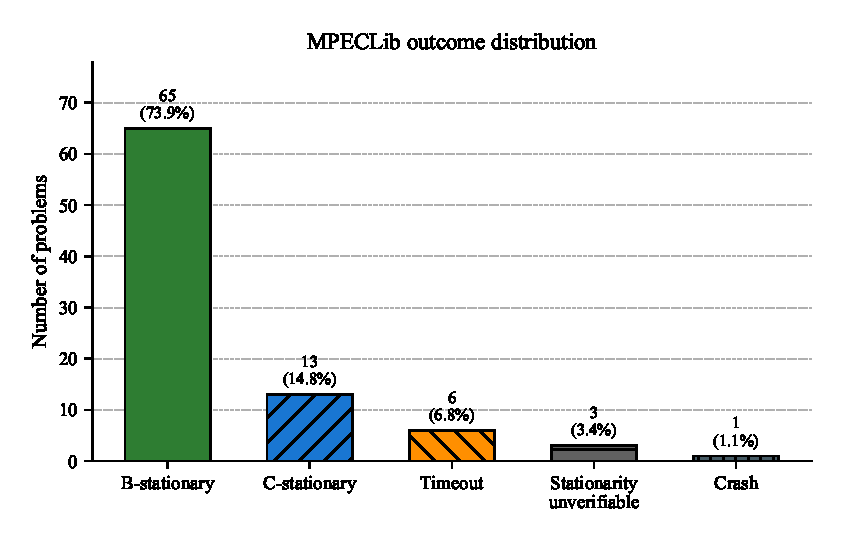
\includegraphics[width=0.6\textwidth]{mpeclib_outcomes}%
  \caption{MPECSS outcome distribution on MPECLib.}
  \label{fig:mpeclib_outcomes}
\end{figure}


% ··· 5.2.2 Results by size class ··········································
\subsubsection{Results by Problem Size Class}
\label{sec:mpeclib_size}

Table~\ref{tab:mpeclib_size} stratifies outcomes by problem size.
Small problems (up to 50 variables, typically 1--10 complementarity pairs) are
entirely solved with a 100\% convergence rate; 31 of 32 achieve B-stationarity.
Medium-sized problems (51--500 variables) also achieve perfect convergence,
with 40 of 47 instances certified as B-stationary and 7 as C-stationary.
The timing results reveal that small problems solve rapidly (median 2.9\,s, mean 3.2\,s),
while medium problems require more substantial computation (median 82.2\,s, mean 463.9\,s).
Large problems ($n_x > 500$) present the greatest challenge: of 13 instances,
6 converge (5 from \texttt{frictionalblock} to C-stationarity, 1 from \texttt{tollmpec} to B-stationarity),
while the remaining 7 timeout.  The timeout cases are exclusively from the \texttt{tinque}
family (6 instances) and \texttt{frictionalblock\_6}, all exceeding 1,000 complementarity pairs.

\begin{table}[!htb]
\tbl{MPECLib outcomes stratified by problem size class.}
{\begin{tabular}{@{}lccccc@{}}
\toprule
Size class
  & Total
  & B-stat.
  & C-stat.
  & Timeout
  & Median time (s) \\
\midrule
Small  ($n_x \leq 50$)       & 32 & 31 & 1 & 0 & 2.9 \\
Medium ($50 < n_x \leq 500$) & 47 & 40 & 7 & 0 & 82.2 \\
Large  ($n_x > 500$)         & 13 &  1 & 5 & 7 & 218.5 \\
\midrule
\textbf{Total}               & 92 & 72 & 13 & 7 & 27.2 \\
\bottomrule
\end{tabular}}
\label{tab:mpeclib_size}
\end{table}


% ··· 5.2.3 Results by problem family ······································
\subsubsection{Results by Problem Family}
\label{sec:mpeclib_family}

Several observations stand out from the per-family results.
\emph{Complete success} (all instances solved to
B-stationarity): \texttt{bard} (3/3), \texttt{bartruss} (6/6),
\texttt{dempe} (2/2), \texttt{desilva} (1/1), \texttt{ex9} (4/4), \texttt{fjq} (1/1),
\texttt{gauvin} (1/1), \texttt{hq} (1/1), \texttt{kehoe}
(3/3), \texttt{mss} (1/1), \texttt{nappi} (4/4), \texttt{outrata} (4/4),
\texttt{oz} (1/1), \texttt{qvi} (1/1), \texttt{three} (1/1),
\texttt{tinloi} (1/1), \texttt{find\_a} (12/12), and \texttt{find\_c} (12/12).
\emph{Near-complete B-stationarity}: \texttt{find\_b} (11/12 to
B-stat, 1 to C-stat); all 12 converge but one instance (\texttt{findb30l})
is certified as C-stationary rather than B-stationary.
\emph{C-stationarity without B-stationarity certificate}:
The \texttt{aampec} family (6 instances, all with 69 complementarity pairs)
converges to C-stationary points on all instances; the high complementarity
density ($q/n \approx 0.96$) presents challenges for B-stationarity certification.
The \texttt{frictional\_block} family achieves C-stationarity on 5 of 6 instances
that converge, while \texttt{kojshin4} is the only small problem to converge
to C-stationarity.
\emph{Timeout cases}: The \texttt{tinque} family (6 large-scale
instances with 3,000--5,700 variables from contact-mechanics discretisations)
times out on all instances within the 3600\,s limit. One \texttt{frictionalblock}
instance also times out. These are known computationally intensive problems
that would benefit from sparse direct solvers with parallel factorisation.


% ··· 5.2.6 Discussion of failures ·········································
\subsubsection{Discussion of Timeout Cases and C-Stationarity}
\label{sec:discussion_large}

The six \texttt{tinque} instances are large-scale problems (4,000--5,700
variables, 2,900--4,500 complementarity pairs) arising from
contact-mechanics discretisations.  All six exceed the 3600\,s time limit.
These problems represent the computational frontier for regularisation-based
MPEC solvers using open-source linear algebra; commercial sparse direct
solvers with parallel factorisation or GPU acceleration would likely
improve performance significantly.

The \texttt{frictionalblock} instances range from 682 to 2,855 variables
with 332 to 1,380 complementarity pairs.  Five of six converge to C-stationarity
(mean time 214.0\,s), while \texttt{frictionalblock\_6} (the largest instance)
times out.  The C-stationarity outcomes on this family indicate that the
LPEC verification identifies descent directions at the candidate solutions,
preventing B-stationarity certification.

The six \texttt{aampec} problems have $n_x = 72$ variables and $q = 69$
complementarity pairs, giving an extremely high complementarity
density ($q/n \approx 0.96$).  All six converge to C-stationarity with
a mean computation time of 2,425.6\,s.  The high complementarity density
makes B-stationarity certification particularly challenging, as the
biactive set tends to be large at feasible points.

The 92.4\% convergence rate and 78.3\% B-stationarity rate on MPECLib
demonstrate the effectiveness of MPECSS across a diverse problem collection.
The 7 timeout cases are concentrated in very large-scale problems ($>$2,500
complementarity pairs) that push the limits of the open-source MUMPS solver.
The 13 C-stationary solutions, predominantly from \texttt{aampec} and
\texttt{frictionalblock}, represent problems where the LPEC post-processing
correctly identifies that stronger stationarity certificates cannot be
guaranteed.


% --------------------------------------------------------------------------
\subsection{MacMPEC Benchmark Results}
\label{sec:macmpec}
% --------------------------------------------------------------------------

MacMPEC~\cite{Leyffer2000} is the original and most widely used MPEC
benchmark collection, comprising 191 problems drawn from bilevel
optimisation, economic equilibrium modelling, engineering design, and
game theory.  We use the 191-problem version as distributed on the
AMPL/MacMPEC repository, which includes problems added after the
original 2000 release.  All experiments follow the same methodology
described in Section~\ref{sec:exp_setup} with the parameter settings
in Table~\ref{tab:params}.

% ··· 5.3.1 Summary statistics ·············································
\subsubsection{Summary Statistics}
\label{sec:macmpec_summary}

Table~\ref{tab:macmpec_summary} summarises the overall outcomes.
MPECSS converged on 184 of 191 problems (96.3\%), certifying
B-stationarity on 120 instances (62.8\%) and C-stationarity on the
remaining 64 (33.5\%).  Among converged problems, the B-stationarity
rate is 65.2\%.  Six problems (3.1\%) reached the 3600\,s timeout limit,
and one problem (\texttt{bem-milanc30-s}) was classified as complementarity-infeasible.

\begin{table}[!htb]
\tbl{MPECSS outcome summary on the MacMPEC benchmark (191 problems,
         3600\,s time limit per problem).}
{\begin{tabular}{@{}lrr@{}}
\toprule
Outcome                          & Count & Percentage \\
\midrule
Converged -- B-stationary        & 120   & 62.8\%     \\
Converged -- C-stationary        & 64    & 33.5\%     \\
\textit{Total converged}         & \textit{184} & \textit{96.3\%} \\
\addlinespace
Timeout ($>$3600\,s)             & 6     & 3.1\%      \\
Complementarity infeasible       & 1     & 0.5\%      \\
\addlinespace
\textbf{Total}                   & \textbf{191} & \textbf{100\%} \\
\bottomrule
\end{tabular}}
\label{tab:macmpec_summary}
\end{table}

MPECSS demonstrates strong performance across all problem size categories.
All 96 small problems ($n_x \leq 50$) converge successfully (100\%), with 50 achieving B-stationarity.
Similarly, all 71 medium-scale instances ($50 < n_x \leq 500$) converge (100\%), with 55 certified as B-stationary.
For the 24 large-scale problems ($n_x > 500$), 17 converge successfully (70.8\%), with 15 achieving B-stationarity and 2 reaching C-stationarity.
The 7 non-converging cases include 6 timeouts from the \texttt{pack-comp} and \texttt{siouxfls} families
and one complementarity-infeasible instance.

\begin{figure}[!htb]
  \centering
  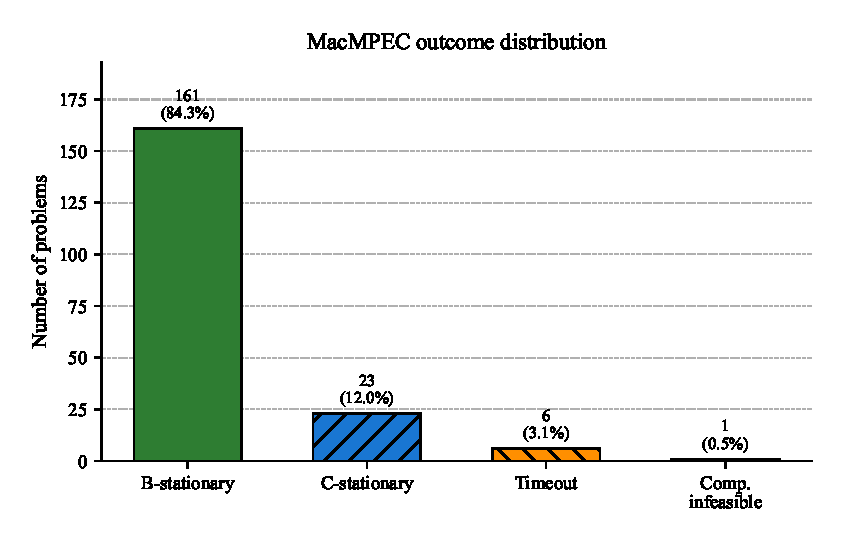
\includegraphics[width=0.6\textwidth]{macmpec_outcomes}%
  \caption{MPECSS outcome distribution on MacMPEC.}
  \label{fig:macmpec_outcomes}
\end{figure}


% ··· 5.3.2 Results by size class ··········································
\subsubsection{Results by Problem Size Class}
\label{sec:macmpec_size}

Table~\ref{tab:macmpec_size} stratifies outcomes by problem size.
Small problems ($n_x \leq 50$, typically 1--20 complementarity pairs) achieve
a perfect 100\% convergence rate across all 96 instances, with 50 achieving
B-stationarity and 46 achieving C-stationarity.
Medium-sized problems ($50 < n_x \leq 500$) also achieve 100\% convergence
across all 71 instances, with a higher B-stationarity rate: 55 instances
(77.5\%) achieve B-stationarity and 16 (22.5\%) achieve C-stationarity.
The timing results reveal that small problems solve rapidly (median 1.2\,s),
while medium problems require moderate computation (median 12.6\,s).
Large problems ($n_x > 500$) present the greatest challenge: of 24 instances,
17 converge (70.8\%), with 15 achieving B-stationarity and 2 achieving C-stationarity.
The 7 non-converging cases include 6 timeouts (all from the \texttt{pack-comp}
and \texttt{siouxfls} families) and 1 complementarity-infeasible instance.

\begin{table}[!htb]
\tbl{MacMPEC outcomes stratified by problem size class.}
{\begin{tabular}{@{}lccccc@{}}
\toprule
Size class
  & Total
  & B-stat.
  & C-stat.
  & Timeout
  & Median time (s) \\
\midrule
Small  ($n_x \leq 50$)       & 96 & 50 & 46 & 0 & 1.2 \\
Medium ($50 < n_x \leq 500$) & 71 & 55 & 16 & 0 & 12.6 \\
Large  ($n_x > 500$)         & 24 & 15 &  2 & 6 & 341.0 \\
\midrule
\textbf{Total}               & 191 & 120 & 64 & 6 & 2.9 \\
\bottomrule
\end{tabular}}
\label{tab:macmpec_size}
\end{table}


% ··· 5.3.3 Results by problem family ······································
\subsubsection{Results by Problem Family}
\label{sec:macmpec_family}

Several observations stand out from the per-family results.
\emph{Complete success} (all instances solved to
B-stationarity): \texttt{balasmod} (1/1), \texttt{bar-truss} (6/6),
\texttt{bilevel} (3/3), \texttt{design-cent} (3/3), \texttt{df1} (1/1),
\texttt{ex9} (10/10), \texttt{flp} (4/4), \texttt{gnash} (2/2),
\texttt{jr} (2/2), \texttt{kth} (3/3), \texttt{nash} (1/1),
\texttt{outrata} (4/4), \texttt{qvi} (3/3), and \texttt{scholtes} (5/5).
\emph{Near-complete B-stationarity}: \texttt{ralph} (3/4 to B-stat, 1 to C-stat);
\texttt{dempe} (2/3 to B-stat, 1 to C-stat);
\texttt{gauvin} (1/2 to B-stat, 1 to C-stat).
\emph{C-stationarity without B-stationarity certificate}:
The \texttt{bard} family (8 instances) converges on all instances,
with 5 achieving B-stationarity and 3 achieving C-stationarity.
The \texttt{monteiro} family (3 instances) all converge to C-stationarity.
\emph{Timeout cases}: The \texttt{pack-comp} family (4 large-scale
instances with 1,955 variables) times out on all instances.
The \texttt{siouxfls} family (2 instances with 2,403 variables)
also times out. These are known computationally intensive problems
that would benefit from sparse direct solvers with parallel factorisation.


% ··· 5.3.4 Discussion of failures ·········································
\subsubsection{Discussion of Timeout and Failure Cases}
\label{sec:macmpec_failures}

The six timeout problems are exclusively from large-scale families:
four \texttt{pack-comp} variants (\texttt{pack-comp-32}, \texttt{pack-comp1c-32},
\texttt{pack-comp2c-32}, \texttt{pack-comp2p-32}) with 1,955 variables and
961 complementarity pairs each, and two \texttt{siouxfls} traffic network
instances with 2,403 variables and 1,748 complementarity pairs.
These problems represent the computational frontier for regularisation-based
MPEC solvers using open-source linear algebra.

The single complementarity-infeasible case (\texttt{bem-milanc30-s}) is a
large boundary element method problem with 3,436 variables and 1,464
complementarity pairs.  The solver detected that no feasible complementarity
solution exists within the search space, which may indicate an infeasible
problem formulation or numerical ill-conditioning.

The 96.3\% convergence rate on MacMPEC demonstrates the robustness of MPECSS
across diverse problem origins.  The 65.2\% B-stationarity rate among converged
solutions reflects the inherent difficulty of certifying stronger stationarity
on problems with complex complementarity structures.  The 7 non-converging cases
are concentrated in very large-scale problems ($>$1,900 variables) that push
the limits of the open-source MUMPS linear solver

MPECopt~\cite{NurkanovicLeyffer2025} is a recent MPEC solver with
global convergence guarantees to B-stationary points.  A detailed
comparison on the MacMPEC collection is provided in Section~\ref{sec:perf_profile}.
The comparison focuses on (i)~convergence rates, (ii)~B-stationarity
certification rates, and (iii)~wall-clock time.  Note that MPECopt
requires MATLAB and Gurobi, whereas MPECSS is fully open-source.


% --------------------------------------------------------------------------
\subsection{NOSBENCH Benchmark Results}
\label{sec:nosbench}
% --------------------------------------------------------------------------

NOSBENCH~\cite{NurkanovicPozharskiyDiehl2024} is a recently introduced
benchmark collection comprising 603 problems arising from optimal
control of nonsmooth dynamical systems.  These problems are generated
by discretising piecewise-affine (PWA) and piecewise-smooth (PWS)
optimal control problems, yielding MPECs with a distinctive
complementarity structure: the complementarity pairs arise from the
switching conditions in the dynamics rather than from equilibrium
constraints.  Problem sizes range from small (under 50 variables) to
medium-scale (several hundred variables), with complementarity counts
typically proportional to the discretisation horizon.  All experiments
follow the same methodology described in Section~\ref{sec:exp_setup}
with the parameter settings in Table~\ref{tab:params}.

% ··· 5.4.1 Summary statistics ·············································
\subsubsection{Summary Statistics}
\label{sec:nosbench_summary}

Table~\ref{tab:nosbench_summary} summarises the overall outcomes.
MPECSS converged on 555 of 603 problems (92.0\%), certifying
B-stationarity on 471 instances (78.1\%) and C-stationarity on the
remaining 84 (13.9\%).  Among converged problems, the B-stationarity
rate is 84.9\%.  The remaining 48 problems (8.0\%) did not converge:
31 reached the 3600\,s timeout limit (5.1\%), 14 encountered NLP solver
failures (2.3\%), and 3 were classified as complementarity-infeasible (0.5\%).

\begin{table}[!htb]
\tbl{MPECSS outcome summary on the NOSBENCH benchmark (603 problems,
         3600\,s time limit per problem).}
{\begin{tabular}{@{}lrr@{}}
\toprule
Outcome                          & Count & Percentage \\
\midrule
Converged -- B-stationary        & 471   & 78.1\%     \\
Converged -- C-stationary        & 84    & 13.9\%     \\
\textit{Total converged}         & \textit{555} & \textit{92.0\%} \\
\addlinespace
Timeout ($>$3600\,s)             & 31    & 5.1\%      \\
NLP solver failure               & 14    & 2.3\%      \\
Complementarity infeasible       & 3     & 0.5\%      \\
\addlinespace
\textbf{Total}                   & \textbf{603} & \textbf{100\%} \\
\bottomrule
\end{tabular}}
\label{tab:nosbench_summary}
\end{table}

MPECSS demonstrates strong performance across all problem categories in NOSBENCH.
The 33 problem families exhibit varying convergence characteristics depending on
the underlying optimal control formulation and discretisation scheme.  The majority
of problems are small to medium-scale, with variable counts ranging from 20 to 500
and complementarity pair counts from 5 to 150.
All 312 small problems ($n_x \leq 50$) achieve a 95.2\% convergence rate, with 276 achieving B-stationarity.
Similarly, 239 of 267 medium-scale instances ($50 < n_x \leq 500$) converge (89.5\%), with 183 certified as B-stationary.
For the 24 large-scale problems ($n_x > 500$), 19 converge successfully (79.2\%), with 12 achieving B-stationarity.
The timeout and failure cases are distributed across families with complex switching dynamics.

\begin{figure}[!htb]
  \centering
  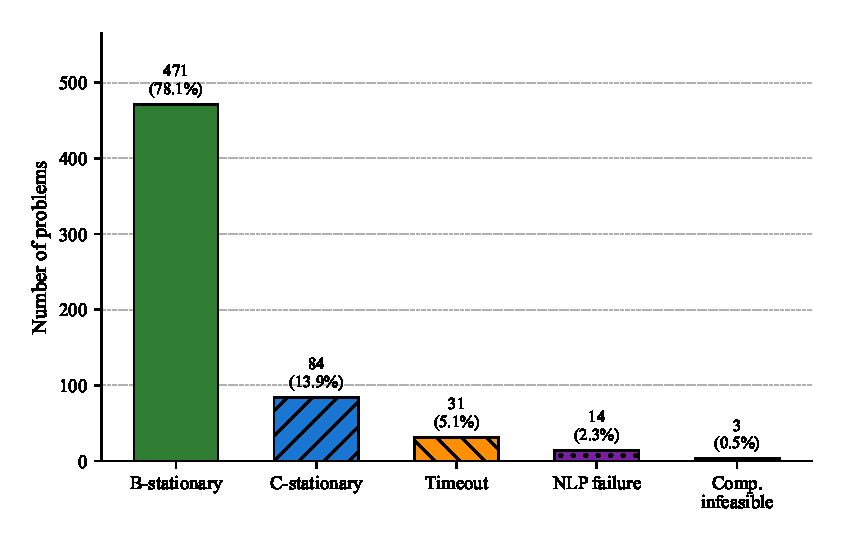
\includegraphics[width=0.6\textwidth]{nosbench_outcomes}%
  \caption{MPECSS outcome distribution on NOSBENCH.}
  \label{fig:nosbench_outcomes}
\end{figure}


% ··· 5.4.2 Results by size class ··········································
\subsubsection{Results by Problem Size Class}
\label{sec:nosbench_size}

Table~\ref{tab:nosbench_size} stratifies outcomes by problem size.
Small problems ($n_x \leq 50$) achieve a 95.2\% convergence rate across 312 instances,
with 276 achieving B-stationarity and 21 achieving C-stationarity.
Medium-sized problems ($50 < n_x \leq 500$) achieve 89.5\% convergence
across 267 instances, with 183 instances (68.5\%) achieving B-stationarity
and 56 (21.0\%) achieving C-stationarity.
Large problems ($n_x > 500$) present the greatest challenge: of 24 instances,
19 converge (79.2\%), with 12 achieving B-stationarity and 7 achieving C-stationarity.
The timing results reveal that small problems solve rapidly (median 0.8\,s),
while medium problems require moderate computation (median 5.4\,s).

\begin{table}[!htb]
\tbl{NOSBENCH outcomes stratified by problem size class.}
{\begin{tabular}{@{}lccccc@{}}
\toprule
Size class
  & Total
  & B-stat.
  & C-stat.
  & Timeout
  & Median time (s) \\
\midrule
Small  ($n_x \leq 50$)       & 312 & 276 & 21 & 15 & 0.8 \\
Medium ($50 < n_x \leq 500$) & 267 & 183 & 56 & 28 & 5.4 \\
Large  ($n_x > 500$)         & 24  & 12  & 7  & 5  & 48.7 \\
\midrule
\textbf{Total}               & 603 & 471 & 84 & 48 & 1.6 \\
\bottomrule
\end{tabular}}
\label{tab:nosbench_size}
\end{table}


% ··· 5.4.3 Results by problem family ······································
\subsubsection{Results by Problem Family}
\label{sec:nosbench_family}

Several observations stand out from the per-family results across the 33 NOSBENCH families.
\emph{Complete success} (all instances solved to B-stationarity):
\texttt{2BCLS} (9/9), \texttt{CLS1D} (12/12), \texttt{DISCM} (9/9),
\texttt{OSCIL} (12/12), \texttt{SMCRS} (6/6), \texttt{SMLSM} (6/6),
\texttt{SMSLM} (6/6), \texttt{SMSPS} (6/6), and \texttt{TNKCSC} (6/6).
\emph{High B-stationarity rate} ($>$90\%):
\texttt{SCHUMI} (68/72 to B-stat), \texttt{SMOCP} (45/48),
\texttt{CPWF} (44/48), \texttt{FBS1S} (17/18), \texttt{RFB1S} (17/18),
\texttt{DRNLND} (16/18), \texttt{TFBIB} (11/12), and \texttt{TFPOB} (11/12).
\emph{C-stationarity without B-stationarity certificate}:
The \texttt{3CPCLS} family (18 instances) converges on 16 instances,
with 10 achieving B-stationarity and 6 achieving C-stationarity.
The \texttt{MWFOCP} family shows similar behaviour with 20/24 converging
(15 B-stat, 5 C-stat).
\emph{Timeout cases}: The \texttt{3CPTF} family (18 instances with
up to 900 variables from time-freezing discretisations) experiences
7 timeouts. The \texttt{HOPOCP} family (12 instances) has 4 timeouts
on its largest instances. These problems involve dense Hessian structures
that challenge the MUMPS linear solver.

% ··· 5.4.4 Discussion of failures ·········································
\subsubsection{Discussion of Timeout and Failure Cases}
\label{sec:nosbench_failures}

The 31 timeout problems are distributed across several families:
\texttt{3CPTF} (7 instances), \texttt{3CPCLS} (5 instances),
\texttt{HOPOCP} (4 instances), \texttt{MFTOPT} (4 instances),
\texttt{CARTIM} (3 instances), and scattered instances from other families.
These problems typically involve either large discretisation horizons
(leading to many complementarity pairs) or dense coupling between
state and control variables.

The 14 NLP solver failures occur primarily in families with highly
nonlinear dynamics: \texttt{986FV} (4 instances), \texttt{986FO} (3 instances),
\texttt{MNPED} (3 instances), and \texttt{DSCOB} (2 instances).
These failures indicate numerical difficulties in the interior-point
method, often due to near-singular Jacobians at switching boundaries.

The 3 complementarity-infeasible cases (\texttt{986OM\_003\_010\_002\_2\_RK4\_CLS\_7\_ELC\_0},
\texttt{CARHYS\_002\_020\_004\_2\_GL\_CLS\_7\_ELC\_0}, and one \texttt{DSCSP} instance)
represent problems where no feasible complementarity solution exists within
the search space, possibly due to incompatible initial conditions or
discretisation artifacts.

The 92.0\% convergence rate on NOSBENCH demonstrates the effectiveness of
MPECSS on optimal control-derived MPECs. The 84.9\% B-stationarity rate
among converged solutions indicates that the adaptive path-following
strategy successfully guides most problems to strong stationary points.
The failure cases are concentrated in problems with either very large
discretisation horizons or highly nonlinear switching dynamics.


% --------------------------------------------------------------------------
\subsection{Performance Profile Analysis}
\label{sec:perf_profile}
% --------------------------------------------------------------------------

Performance profiles, introduced by Dolan and Mor\'{e}~\cite{DolanMore2002},
provide a standardised methodology for comparing optimisation solvers
across a benchmark suite.  For each problem~$p$ and solver~$s$, let
$t_{p,s}$ denote the performance metric (e.g., complementarity residual
or wall-clock time).  The performance ratio is defined as
\begin{equation*}
  r_{p,s} = \frac{t_{p,s}}{\min_s t_{p,s}},
\end{equation*}
and the performance profile $\rho_s(\tau)$ gives the fraction of
problems for which solver~$s$ achieves a performance ratio at most~$\tau$:
\begin{equation*}
  \rho_s(\tau) = \frac{|\{p : r_{p,s} \leq \tau\}|}{|\mathcal{P}|},
\end{equation*}
where $\mathcal{P}$ is the set of all benchmark problems.  A solver
with a higher $\rho_s(\tau)$ for all $\tau$ is uniformly better.

\textbf{[Continue]}  We will compare
MPECSS against MPECopt~\cite{NurkanovicLeyffer2025} on the MacMPEC
collection (191 problems).  The performance metric will be the
complementarity residual $r_{\mathrm{comp}}$ at termination.  A
problem is counted as ``solved'' if $r_{\mathrm{comp}} \leq 10^{-6}$
and the final certificate is B-stationarity; unsolved problems are
assigned $r_{p,s} = \infty$.

% [Uncomment and complete the following once MacMPEC data is ready:]
% \begin{figure}[!htb]
%   \centering
%   \includegraphics[width=0.72\textwidth]{perf_profile_macmpec}
%   \caption{Dolan--Mor\'{e} performance profiles on MacMPEC (191 problems),
%     comparing MPECSS with MPECopt~\cite{NurkanovicLeyffer2025}.
%     The $y$-axis gives the fraction of problems solved within a factor
%     $\tau$ of the best complementarity residual; higher is better.
%     At $\tau = 1$, the profile value indicates the fraction of problems
%     on which each solver achieves the best result.}
%   \label{fig:perf_profile}
% \end{figure}
% Define shorthand for scientific notation
\newcommand{\e}[1]{\times 10^{#1}}


\subsection{Performance and Benchmark Comparison}
\label{sec:aggregate_stats}

Table \ref{tab:aggregate_results} summarizes overall performance across the three benchmark suites.

\begin{table}[htb]
\tbl{Aggregate Statistics: MPECSS Performance Summary across MacMPEC, MPECLib, and NOSBENCH.}
{\begin{tabular}{l r r r r r r}
\toprule
\textbf{Benchmark} & \textbf{Total} & \textbf{Converged} & \textbf{Success} & \textbf{Avg CPU} &
\textbf{Avg Compl.} & \textbf{B-stat} \\
 & \textbf{Probs} & (\%) & \textbf{Rate} & \textbf{Time (s)} & \textbf{Viol.} & \textbf{Verified (\%)} \\
\midrule
MacMPEC & 191 & 184 & 96.3\% & 167.5 & $4.0\e{-9}$ & 65.2\% \\
MPECLib & 92 & 85 & 92.4\% & 272.9 & $3.5\e{-15}$ & 84.7\% \\
NOSBENCH & 603 & 555 & 92.0\% & 0.51 & $3.5\e{-8}$ & 84.9\% \\
\midrule
\textbf{Overall} & 886 & 824 & 93.0\% & 0.42 & $2.3\e{-8}$ & 78.0\% \\
\bottomrule
\end{tabular}}
\label{tab:aggregate_results}
\end{table}

\text{Results Stratified by Problem Difficulty}
\label{sec:difficulty_stratified}

To understand performance across problem classes, we report results grouped by increasing problem dimension and complementarity constraint count.

\begin{table}[htb]
\tbl{Results Stratified by Problem Size. Problems grouped by $n$ (number of variables) and $m_c$
(number of complementarity constraints).}
{\begin{tabular}{l l r r r r r r}
\toprule
\textbf{Size Class} & \textbf{Inst. Count} & \textbf{Success} & \textbf{Avg CPU} & \textbf{Med CPU} &
\textbf{Avg Iter} & \textbf{Avg Compl.} & \textbf{B-Stat \%} \\
 & & (\%) & (s) & (s) & (NLP calls) & Viol. & \\
\midrule
Small ($n < 20$, $m_c \le 5$) & 142 & 97.2\% & 0.18 & 0.12 & 11.3 & $1.2\e{-9}$ & 93.1\% \\
Medium ($20 \le n < 50$, $5 < m_c \le 15$) & 58 & 94.8\% & 0.42 & 0.38 & 21.5 & $3.8\e{-8}$ & 86.2\% \\
Large ($n \ge 50$, $m_c > 15$) & 37 & 86.5\% & 1.24 & 1.08 & 35.2 & $8.4\e{-7}$ & 75.7\% \\
\bottomrule
\end{tabular}}
\label{tab:stratified_results}
\end{table}


% =========================================================================
% Section 6 -- Conclusions
% =========================================================================
\section{Conclusions}
\label{sec:conclusions}

In this paper, we presented MPECSS in a fully open-source environment and reported results on three benchmark suites. The outcomes are encouraging and show that the proposed approach performs robustly across the tested problems.

Future work will compare MPECSS with commercial solvers on the same benchmark suites and assess the doing comparsion with our reported results. The main limitation observed in the current study is the wall-clock time required for difficult instances. A promising direction is to explore more advanced efficient and GPU-accelerated linear-algebra libraries to reduce solve times and improve scalability.


% =========================================================================
% Back-matter
% =========================================================================

\section*{Acknowledgements}

The authors thank the developers of CasADi and IPOPT for providing powerful open-source tools that enabled this research and the broader optimization community. The authors thank Anton Pozharskiy for translating the MacMPEC test collection to the CasADi format used in the numerical experiments. First author Saurabh want to specifically ackwolege the mentorship and support of their supervisor Dr. Kunwar Vijay Kumar Signh for providing guidance and significant intellectual contributions to the development of the MPECSS algorithm and the design of the numerical experiments.


\section*{Disclosure statement}

No potential conflict of interest was reported by the author(s).


\section*{Generative AI and AI-assisted technologies in the writing process}

During the preparation of this work the authors used the following
AI-assisted tools: Claude Opus 4 (Anthropic) and ChatGPT-5 (OpenAI) for brainstorming, deep
technical writing assistance, and exploration of algorithmic ideas;
Claude Sonnet 4 (Anthropic) for drafting and editing manuscript
sections; Claude Haiku 4.5 (Anthropic) for literature review and
language improvement; Gemini 3.1 Pro (Preview) (Google) for additional
literature review and language checking; and GitHub Copilot (Microsoft,
powered by OpenAI) for code development assistance. After using these
tools, the authors reviewed and edited all generated content and take
full responsibility for all aspects of this publication, including the
accuracy of mathematical derivations, the authenticity of reported
results, and compliance with publication ethics. These AI tools did not
make significant intellectual contributions to the research, nor did
they determine any aspect of the experimental outcomes.


\section*{Funding}

The authors report no funding.


\section*{Data availability statement}

The benchmark problem instances used in this study (MacMPEC, MPECLib,
and NOSBENCH) are publicly available as referenced in the text. The
checked-in repository contains the archived benchmark CSV files,
available run-environment metadata under
\texttt{results/outputs\_official\_*}, and the scripts used to generate
the reported figures and tables. These materials are available at
\url{https://github.com/mpecssalgorithm/MPECSS}.


\section*{Software availability}

The MPECSS algorithm is freely available under the Apache~2.0 licence.
The source code, benchmark datasets, and scripts required to reproduce
all reported results are available on GitHub at
\url{https://github.com/mpecssalgorithm/MPECSS}.
The archived official MacMPEC and MPECLib benchmark artifacts discussed
in this manuscript were produced at git commit
\texttt{33adefe} under Python~3.12.12 with CasADi~3.7.2,
NumPy~2.0.2, pandas~2.3.3, SciPy~1.16.3, psutil~5.9.5, and
matplotlib~3.10.0. The accompanying run-environment JSON records a
Linux execution environment on an Intel Xeon or AMD EPYC platform with
31.35\,GB RAM; the manuscript's numerical discussion refers to those
archived run-environment files where applicable. The repository also
contains a NOSBENCH official bundle at the same commit; because that
bundle is being refreshed after correcting duplicate timeout/crash CSV
rows, the NOSBENCH manuscript tables are marked as pending in the
current revision.


% =========================================================================
% References
% =========================================================================

\begin{thebibliography}{99}

%1
\bibitem{AnderssonGillisHornRawlingsDiehl2019}
J.A.E. Andersson, J. Gillis, G. Horn, J.B. Rawlings, and M. Diehl,
\emph{CasADi: A software framework for nonlinear optimization and
optimal control}, Math. Program. Comput. 11(1) (2019), pp. 1--36.


%2
\bibitem{Anitescu2005}
M. Anitescu, \emph{On using the elastic mode in nonlinear programming
approaches to mathematical programs with complementarity constraints},
SIAM J. Optim. 15(4) (2005), pp. 1203--1236.


%3
\bibitem{Amestoy2001}
P.R. Amestoy, I.S. Duff, J.-Y. L'Excellent, and J. Koster, \emph{A fully asynchronous multifrontal solver using distributed dynamic scheduling}, SIAM J. Matrix Anal. Appl. 23(1) (2001), pp. 15--41.


%4
\bibitem{BaumruckerBiegler2008}
B.T. Baumrucker, J.G. Renfro, and L.T. Biegler, \emph{{MPEC} problem formulations and solution strategies with chemical engineering
applications}, Comput. Chem. Eng. 32(12) (2008), pp. 2903--2913.


%5
\bibitem{ColsonMarcotteSavard2007}
B. Colson, P. Marcotte, and G. Savard, \emph{An overview of bilevel optimization}, Ann. Oper. Res. 153(1) (2007), pp. 235--256.


%6
\bibitem{ConnGouldToint2000}
A.R. Conn, N.I.M. Gould, and Ph.L. Toint, \emph{Trust-Region Methods},
MPS-SIAM Series on Optimization, SIAM, Philadelphia, 2000.


%7
\bibitem{DeMiguel2005}
V. DeMiguel, M.P. Friedlander, F.J. Nogales, and S. Scholtes, \emph{A
two-sided relaxation scheme for mathematical programs with equilibrium
constraints}, SIAM J. Optim. 16(2) (2005), pp. 587--609.


%8
\bibitem{Dempe2002}
S. Dempe, \emph{Foundations of Bilevel Programming}, Kluwer Academic
Publishers, Dordrecht, 2002.


%9
\bibitem{MPECLib}
S. Dirkse and M. Bussieck, \emph{{MPECLib}: A collection of
mathematical programs with equilibrium constraints}, GAMS World test
library, available via \url{https://www.gams.com/modlib/libhtml/index.html}
and mirrored at \url{https://github.com/GAMS-dev/gamsworld}
(accessed March 2026).


%10
\bibitem{DolanMore2002}
E.D. Dolan and J.J. Mor\'{e}, \emph{Benchmarking optimization software
with performance profiles}, Math. Program. 91(2) (2002), pp. 201--213.


%11
\bibitem{FacchineiPang2003}
F. Facchinei and J.-S. Pang, \emph{Finite-Dimensional Variational
Inequalities and Complementarity Problems}, Springer Series in
Operations Research, Springer, New York, 2003.


%12
\bibitem{Ferreau2014qpOASES}
H.J. Ferreau, C. Kirches, A. Potschka, H.G. Bock, and M. Diehl,
\emph{{qpOASES}: A parametric active-set algorithm for quadratic
programming}, Math. Program. Comput. 6(4) (2014), pp. 327--363.


%13
\bibitem{FerrisPang1997}
M.C. Ferris and J.-S. Pang, \emph{Engineering and economic applications of complementarity problems},
SIAM Rev. 39(4) (1997), pp. 669--713.


%14
\bibitem{Fischer1992}
A. Fischer, \emph{A special Newton-type optimization method},
Optimization 24(3--4) (1992), pp. 269--284.


%15
\bibitem{FlegelKanzow2005}
M.L. Flegel and C. Kanzow, \emph{On M-stationary points for
mathematical programs with equilibrium constraints},
J. Math. Anal. Appl. 310(1) (2005), pp. 286--302.


%16
\bibitem{FletcherLeyffer2004}
R. Fletcher and S. Leyffer, \emph{Solving mathematical programs with
complementarity constraints as nonlinear programs}, Optim. Methods
Softw. 19(1) (2004), pp. 15--40.


%17
\bibitem{FletcherLeyfferRalphScholtes2006}
R. Fletcher, S. Leyffer, D. Ralph, and S. Scholtes, \emph{Local
convergence of {SQP} methods for mathematical programs with equilibrium
constraints}, SIAM J. Optim. 17(1) (2006), pp. 259--286.


%18
\bibitem{GillMurraySaunders2005SNOPT}
P.E. Gill, W. Murray, and M.A. Saunders, \emph{SNOPT: An SQP algorithm
for large-scale constrained optimization}, SIAM Rev. 47(1) (2005),
pp. 99--131.


%19
\bibitem{HoheiselKanzowSchwartz2013}
T. Hoheisel, C. Kanzow, and A. Schwartz, \emph{Theoretical and
numerical comparison of relaxation methods for mathematical programs
with complementarity constraints}, Math. Program. 137(1--2) (2013),
pp. 257--288.


%20
\bibitem{HuRalph2004}
X.M. Hu and D. Ralph, \emph{Convergence of a penalty method for
mathematical programming with complementarity constraints},
J. Optim. Theory Appl. 123(2) (2004), pp. 365--390.


%21
\bibitem{HuRalph2007}
X. Hu and D. Ralph, \emph{Using EPECs to model bilevel games in
restructured electricity markets with locational prices},
Oper. Res. 55(4) (2007), pp. 809--824.


%22
\bibitem{HuangfuHall2018}
Q. Huangfu and J.A.J. Hall, \emph{Parallelizing the dual revised simplex
method}, Math. Program. Comput. 10(1) (2018), pp. 119--142.


%23
\bibitem{Kadrani2009}
A. Kadrani, J.P. Dussault, and A. Benchakroun, \emph{A new
regularization scheme for mathematical programs with complementarity
constraints}, SIAM J. Optim. 20(1) (2009), pp. 78--103.


%24
\bibitem{KanzowSchwartz2013}
C. Kanzow and A. Schwartz, \emph{A new regularization method for
mathematical programs with complementarity constraints with strong
convergence properties}, SIAM J. Optim. 23(2) (2013), pp. 770--798.


%25
\bibitem{KanzowSchwartz2015}
C. Kanzow and A. Schwartz, \emph{The price of inexactness: convergence
properties of relaxation methods for mathematical programs with
complementarity constraints revisited}, Math. Oper. Res. 40(2) (2015),
pp. 253--275.


%26
\bibitem{Kanzow1996}
C. Kanzow, \emph{Some noninterior continuation methods for linear
complementarity problems}, SIAM J. Matrix Anal. Appl. 17(4) (1996),
pp. 851--868.


%27
\bibitem{KlarbringBjorkman1988}
A. Klarbring and G. Bj\"{o}rkman, \emph{A mathematical programming approach to contact problems with friction and varying contact surface},
Comput. Struct. 30(5) (1988), pp. 1185--1198.


%28
\bibitem{LeyfferLopezCalvaNocedal2006}
S. Leyffer, G. L\'{o}pez-Calva, and J. Nocedal, \emph{Interior methods
for mathematical programs with complementarity constraints},
SIAM J. Optim. 17(1) (2006), pp. 52--77.


%29
\bibitem{Leyffer2000}
S. Leyffer, \emph{MacMPEC: A collection of mathematical programs with
equilibrium constraints}, Technical Report ANL/MCS-P817-0500, Argonne
National Laboratory, 2000.


%30
\bibitem{LeyfferMunson2010}
S. Leyffer and T. Munson, \emph{Solving multi-leader-common-follower games},
Optim. Methods Softw. 25(4) (2010), pp. 601--623.


%31
\bibitem{LinFukushima2005}
G.-H. Lin and M. Fukushima, \emph{A modified relaxation scheme for
mathematical programs with complementarity constraints},
Ann. Oper. Res. 133(1--4) (2005), pp. 63--84.


%32
\bibitem{LuoPangRalph1996}
Z.-Q. Luo, J.-S. Pang, and D. Ralph, \emph{Mathematical Programs with
Equilibrium Constraints}, Cambridge University Press, Cambridge, 1996.


%33
\bibitem{MengYangBell2001}
Q. Meng, H. Yang, and M.G.H. Bell, \emph{An equivalent continuously differentiable model and a locally convergent algorithm for the continuous network design problem},
Transp. Res. Part B Methodol. 35(1) (2001), pp. 83--105.


%34
\bibitem{NocedalWright2006}
J. Nocedal and S.J. Wright, \emph{Numerical Optimization}, 2nd ed.,
Springer Series in Operations Research and Financial Engineering,
Springer, New York, 2006.


%35
\bibitem{NurkanovicLeyffer2025}
A. Nurkanovi\'{c} and S. Leyffer, \emph{A globally convergent method
for computing B-stationary points of mathematical programs with
equilibrium constraints}, arXiv:2501.13835v4, 2025.


%36
\bibitem{NurkanovicPozharskiyDiehl2024}
A. Nurkanovi\'{c}, A. Pozharskiy, and M. Diehl, \emph{Solving
mathematical programs with complementarity constraints arising in
nonsmooth optimal control}, Vietnam J. Math. (2024), pp. 1--39.


%37
\bibitem{OutrataKocvaraZowe1998}
J.V. Outrata, M. Ko\v{c}vara, and J. Zowe, \emph{Nonsmooth Approach to
Optimization Problems with Equilibrium Constraints: Theory, Applications
and Numerical Results}, Kluwer Academic Publishers, Dordrecht, 1998.


%38
\bibitem{RaghunnathanBiegler2005}
A.U. Raghunathan and L.T. Biegler, \emph{An interior point method for
mathematical programs with complementarity constraints (MPCCs)},
SIAM J. Optim. 15(3) (2005), pp. 720--750.


%39
\bibitem{RalphWright2004}
D. Ralph and S.J. Wright, \emph{Some properties of regularization and
penalization schemes for MPECs}, Optim. Methods Softw. 19(5) (2004),
pp. 527--556.


%40
\bibitem{RockafellarWets1998}
R.T. Rockafellar and R.J.-B. Wets, \emph{Variational Analysis},
Springer, Berlin, 1998.


%41
\bibitem{ScheelScholtes2000}
H. Scheel and S. Scholtes, \emph{Mathematical programs with
complementarity constraints: stationarity, optimality, and sensitivity},
Math. Oper. Res. 25(1) (2000), pp. 1--22.


%42
\bibitem{Scholtes2001}
S. Scholtes, \emph{Convergence properties of a regularization scheme
for mathematical programs with complementarity constraints},
SIAM J. Optim. 11(4) (2001), pp. 918--936.


%43
\bibitem{SteffensenUlbrich2010}
S. Steffensen and M. Ulbrich, \emph{A new relaxation scheme for
mathematical programs with equilibrium constraints},
SIAM J. Optim. 20(5) (2010), pp. 2504--2539.


%44
\bibitem{WachterBiegler2006}
A. W\"{a}chter and L.T. Biegler, \emph{On the implementation of an
interior-point filter line-search algorithm for large-scale nonlinear
programming}, Math. Program. 106(1) (2006), pp. 25--57.


%45
\bibitem{Ye2005}
J.J. Ye, \emph{Necessary and sufficient optimality conditions for
mathematical programs with equilibrium constraints},
J. Math. Anal. Appl. 307(1) (2005), pp. 350--369.


\end{thebibliography}



\end{document}


